\documentclass[stu, 12pt, noextraspace, floatsintext]{apa7} 
\usepackage[utf8]{inputenc}
\usepackage[english,spanish]{babel}
\usepackage[final]{microtype}
\usepackage{mathptmx} % times new roman

% figures path
\graphicspath{{images/}}
\usepackage{pdfpages}

% figures doublespace
\captionsetup{skip=0pt, font=doublespacing}
\usepackage{etoolbox}
% make toc with apa 7 line space. This uses etoolbox
\addtocontents{toc}{\protect\renewcommand*\protect\addvspace[1]{}}

% max layer into index
% -1 part     1 section     3 subsubsection  5 subparagraph 
% 0 chapter  2 subsection  4 paragraph
\setcounter{tocdepth}{5} 

% apa rule for spacing
\usepackage{setspace}
% apa rule for indent
\setlength{\parindent}{1.27cm}

% plain pagestyle for other pages
\fancypagestyle{otherplain}{
\fancyhf{}
\fancyheadoffset{0cm}
\renewcommand{\headrulewidth}{0pt}
\renewcommand{\footrulewidth}{0pt}
\fancyhead[R]{\thepage}
}

% code package
\usepackage{minted}
\usepackage{listings}
\usemintedstyle[Python]{colorful}
\usemintedstyle[Console]{bw}
\setminted{fontsize=\footnotesize,linenos, breaklines=true,numberblanklines=false}
% minted code centered
\RecustomVerbatimEnvironment{Verbatim}{BVerbatim}{}

% library package
\usepackage[style=apa,sortcites=true,sorting=ynt,backend=biber]{biblatex}
\addbibresource{references.bib}
\usepackage[autostyle]{csquotes}

% math package
\usepackage{amsmath, amsthm, amssymb}

% graphics and fig
\usepackage{bigstrut}
\usepackage{color}
\usepackage{colortbl}
\usepackage{siunitx}

\usepackage{multirow}
\usepackage{booktabs}
\usepackage{pdflscape}
\usepackage{longtable}

\usepackage{csvsimple}
\usepackage{pgfplots}
\pgfplotsset{compat=1.16}
\usepackage{tikz}
\usetikzlibrary{calc}

% english quotation
\DeclareQuoteStyle{english}
    {\textquotedblleft}
    [\textquotedblleft]
    {\textquotedblright}
        [0.05em]
    {\textquoteleft}
    [\textquoteleft]
    {\textquoteright}

\setquotestyle{english}

\hypersetup{hidelinks}

\usepackage{adjustbox}
% ---------------------------

\begin{document}


\begin{titlepage}
    \begin{center}
        \textbf{Voorspelling, aplicación de escritorio para Aprendizaje de Máquina Supervisado}
        
        \vfill
        
        Autores:\\
        \textbf{
        Iván David Rey Rueda y
        German Francisco Diaz Figueredo}
        
        \vfill
        
        Universidad de Santander\\
        Facultad de Ingenierías\\
        Ingeniería de Software\\
        Bucaramanga, Santander\\
        2020
    \end{center}
\thispagestyle{otherplain}   
\pagebreak
    
\begin{center}
        \textbf{Voorspelling, aplicación de escritorio para Aprendizaje de Máquina Supervisado}
        
        \vfill
        
        Autores:\\
        \textbf{
        Iván David Rey Rueda y German Francisco Diaz Figueredo}
        
        \vfill
        Trabajo de grado presentado como requisito parcial para obtener título de Ingeniero de Software
        
        \vfill
        
        Directora de proyecto:\\
        \textbf{Doctora Nydia Paola Rondón Villarreal}
        
        \vfill
        
        Universidad de Santander\\
        Facultad de Ingenierías\\
        Ingeniería de Software\\
        Bucaramanga, Santander\\
        2020
        
    \end{center}
\thispagestyle{otherplain}   
\end{titlepage} % cover page
\setcounter{page}{3} % magic number to make cover page count as first page

\renewcommand{\contentsname}{Índice general}
\tableofcontents % general index

\clearpage
\let\oldnumberline\numberline % Copy \numberline into \oldnumberline
\renewcommand{\numberline}[1]{\hspace*{-1.5em}} % Remove number argument 
\listoffigures % fig index
\let\numberline\oldnumberline % Restore \numberline (if needed)

%\clearpage
%\let\oldnumberline\numberline % Copy \numberline into \oldnumberline
%\renewcommand{\numberline}[1]{\hspace*{-1.5em}} % Remove number argument 
%\listoftables % fig index
%\let\numberline\oldnumberline % Restore \numberline (if needed)

\clearpage
\section*{Abstract} % doc abstract
\noindent{The lack of skills and knowledge in a specific subject, as it is in this case Machine Learning, leads students to change their learning path in most cases, or in the best case scenario if students keep studying Artifical Intelligence, the biggest obstacle on the way are applications that do not  meet their academic needs and have high cost prices. It is for such reasons that students are forced to use these means until the free trial runs out, otherwise they have to resort to traditional means such as creating source code to train models, which is not a doable options due to the lack of knowledge that students have in their first years of professional training. It is mainly for these reasons that in the present project it is planned to develop a desktop application for the \textit{Windows} 10 x64 operative system in the course of eight months starting from August 2020, with the purpose of allowing model selection, hyper-parameters, training and prediction based on the supplied dataset to students in their first years of academic courses in careers such as Software Engineering, Systems Engineering and Computer Science, throughout and easy-to-understand user interface and detailed documentation of the built-in functions.}

\noindent{\textbf{Keywords: }Supervised Machine Learning, Desktop app, Python.}

\clearpage
\section*{Resumen} % doc abstract spanish
\noindent{La falta de habilidades y conocimientos en un tema específico, como lo es en este caso el Aprendizaje de Máquina lleva a los estudiantes a cambiar su ruta de aprendizaje en la mayoría de los casos, o si en definitiva se continúa por el camino de la Inteligencia Artificial, el mayor obstáculo en el camino son las aplicaciones con costos elevados que no satisfacen las necesidades de aprendizaje. Por tales motivos, los estudiantes se ven obligados a utilizar esos medios hasta agotar la prueba gratuita o tener que recurrir a medios tradicionales como crear código fuente para entrenar los modelos, opción poco factible debido a la falta de conocimientos que presentan los estudiantes en sus primeros años de formación profesional. Por lo tanto, en el presente proyecto se planteó desarrollar una aplicación de escritorio para el sistema operativo Windows 10 x64 en el transcurso de 8 meses a partir de Agosto del 2020, con el fin de permitir a estudiantes en su primeros años de formación académica en carreras como Ingeniería de Software, Sistemas, Informática y Computación, la selección del modelo, hiperparámetros, entrenamiento y predicción con base al conjunto de datos suministrado, por medio de una interfaz de usuario sencilla de comprender y documentación detallada de las funciones incorporadas.}

\textit{Palabras clave}: Aprendizaje de Máquina Supervisado, Aplicación de escritorio, Python.

\clearpage
\section{Introducción}
\input{chapters/introducción}

\clearpage
\section{Planteamiento del problema}
Programar es una de las tantas habilidades que un estudiante de Ingeniería de Software, Sistemas o Computación debe dominar, junto a otras áreas como: cálculo, álgebra, estadística y física \parencite{Ozmen2014}. \textcite{Tan2009} en su estudio manifiestan que aprender un lenguaje de programación no es tarea fácil, y además es un proceso largo y tedioso de por lo menos algunos meses, se requiere mucha dedicación, especialmente para los estudiantes de primer año, ya que en ese punto los programadores novatos carecen de las habilidades necesarias para resolver problemas.

Debido a que la programación es un requisito obligatorio, aún con todos los obstáculos que presenta para los estudiantes de carreras afines, autores como \textcite{McCracken2001} en su estudio titulado ``\textit{A multi-national, multi-institutional study of assessment of programming skills of first-year CS students}'' se formulan la pregunta: ¿Los estudiantes cumplen realmente con los conocimientos necesarios?. En el estudio previamente mencionado, los estudiantes obtuvieron en promedio 22.9 de 110 puntos con una desviación estándar de 25.2, mucho más bajo de lo que esperaban en un principio, por diferentes motivos tales como: los estudiantes no evalúan todas las rutas del programa, el código no es legible, malas prácticas, falta de pruebas de software y problemas relacionados con pobre capacidad matemática. De igual forma \textcite{Krpan2015} manifiestan que aprender a programar al nivel universitario es todo un reto para los estudiantes, especialmente para aquellos sin ninguna experiencia previa en algún lenguaje, y por otro lado, también hay que agregar la dificultad añadida de las primeras materias que cursa todo estudiante en su ciclo básico. En este periodo Krpan expresa que se encuentra el mayor rango de deserción, siendo una de las principales razones la dificultad con el pensamiento abstracto. Por esas y demás razones, los docentes y profesionales tienen la tarea de diseñar o implementar formas de enseñanza alternativas que mejoren significativamente las habilidades de programación de los estudiantes, y de igual forma incorporar nuevos conocimientos y conceptos que les permitan entender los lenguajes de programación como si de su primera lengua se tratase. Desafortunadamente aún no hay una solución definitiva, a pesar de que a lo largo de los años se han intentado establecer nuevas metodologías para el aprendizaje.

Los estudiantes que se adentran al mundo de la programación, en particular en un lenguaje como Python, al nivel universitario encuentran una serie de desafíos, desde problemas simples con el código, hasta problemas debido a conceptos mal establecidos \parencite{Piwek2020}. Es esta falta de habilidades y conocimientos en un tema específico, como en este caso el Aprendizaje de Máquina, la razón que conduce a los estudiantes en sus primeros años de formación profesional a afrontar tres situaciones particulares
\begin{seriate}
    \item renunciar
    \item cambiar completamente el enfoque profesional
    \item toparse con aplicaciones que no satisfacen las necesidades de aprendizaje, y que en muchos casos no son asequibles.
\end{seriate}
Por las razones anteriormente mencionadas, los estudiantes de carreras profesionales como Ingeniería de Software, Sistemas, Informática y Computación, que desean desarrollar sus propios modelos de Aprendizaje de Máquina y que además no precisan de las habilidades necesarias para escribir su propio código, se ven en la necesidad de recurrir a las aplicaciones disponibles en la web. Sin embargo, la gran mayoría de las aplicaciones son pagas o en algunos casos con pruebas gratuitas muy limitadas, por lo que después de unos pocos usos se hace necesaria una suscripción, a causa de que es necesario como mínimo generar los ingresos para mantener en servicio la aplicación, situación que es más evidente en el caso de las aplicaciones web que en las de escritorio.




\clearpage
\section{Justificación}
\input{chapters/justificación}

\clearpage
\section{Objetivo}
\subsection{Objetivo general}
Desarrollar una aplicación de escritorio para Aprendizaje de Máquina Supervisado en el sistema operativo Windows 10 x64, que permita a los usuarios la selección del modelo, hiperparámetros, entrenamiento y predicción con base al conjunto de datos suministrado. 

\subsection{Objetivos específicos}
\begin{APAitemize}
    \item Establecer los requerimientos funcionales y no funcionales de la aplicación de Aprendizaje de Máquina Supervisado.
    \item Diseñar la interfaz gráfica y el \textit{back-end} de la aplicación, con referencia a patrones y buenas prácticas para su construcción.
    \item Desarrollar el código fuente de la aplicación con base al diseño establecido. 
    \item Ejecutar pruebas de validación, integración y regresión, garantizando el funcionamiento y calidad de la aplicación.
    \item Generar la versión ejecutable dada la completitud de las fases de requerimientos, diseño, código, documentación y pruebas.
\end{APAitemize}




\clearpage
\section{Marco teórico}
\subsection{Python}
\subsubsection{Definición}
Según la documentación de Python \parencite{Pythondoc} este lenguaje es la combinación de velocidad y una sintaxis fácil de comprender, tiene múltiples librerías, puede ejecutarse en diferentes sistemas operativos y es extensible a otros lenguaje como C y C++. Python \parencite{Python3} es un lenguaje de programación de alto nivel interpretado multiparadigma, es decir, no hay nada que impida a los desarrolladores programar utilizando otros paradigmas, tales como lo son la programación procedural y funcional.

Por lo general, este lenguaje es utilizado en aplicaciones de consola, dado que no cuenta con la facilidad de otros lenguajes como PHP y JavaScript para tener acceso a lenguajes de hipertexto. En esos casos específicos donde Python es el lenguaje utilizado en el \textit{back-end}, se emplean \textit{frameworks} como Electron o librerías como EEl para comunicar las entradas del usuario a Python y luego regresar una salida que pueda ser comprendida en un ambiente con interfaz de usuario que utilice HTML y CSS para el \textit{front-end}. No obstante, cuando los requerimientos de una aplicación necesitan de un ambiente nativo de escritorio y no es necesario utilizar tecnologías relacionadas a ambientes web, es entonces cuando otros \textit{framework} que utilizan Python tanto para el \textit{front-end} como para el \textit{back-end} son una opción más óptima, dado que no se necesitan de otros lenguajes que aumentan la complejidad del problema. 

\subsubsection{Librerías}
Conforme a lo mencionado en la documentación de Python \parencite{Pythondoc}, la librería estándar de este lenguaje contiene módulos originalmente construidos en C que aportan funcionalidades como el acceso a las rutas del sistema, que de otro modo no serían posible en este lenguaje. De igual forma, la librería estándar también tiene módulos desarrollados originalmente en Python, los cuales aportan soluciones para los problemas regulares que se enfrentan los desarrolladores en este lenguaje.

Algunos de los módulos por defecto en Python proveen varias interfaces específicas del lenguaje, mientras que otros son del sistema operativo o módulos relacionados a ambientes web. Aunque gran parte de las librerías se encuentran disponibles directamente en el lenguaje, hay otras que necesitan primero ser descargadas e instaladas en el sistema, ya sea en un entorno virtual o en la instalación base de la distribución elegida a través de pip, el cual es el paquete estándar para administrar los módulos en Python.

Los módulos, paquetes y librerías que se utilizan en mayor medida en este proyecto de Aprendizaje de Máquina Supervisado son: numpy, pandas, scikitlearn, mljar-supervised, xgboost, tensorflow, seaborn, Pyinstaller, PyQt5, abc, random y json. 

\begin{APAitemize}
    \item Numpy: se utiliza para trabajar con vectores y matrices propias del álgebra linear en Python, en vez de utilizar las listas y tuplas que ofrece por defecto el lenguaje.
    \item Pandas: está diseñado para manipular estructuras de datos tabulares y multidimensionales, así como la información que contienen archivos csv y tsv.
    \item Scikitlearn: es una librería de acceso libre que utiliza principalmente Numpy y pandas. Esta librería proporciona una implementación de varios algoritmos conocidos de Aprendizaje de Máquina, al mismo tiempo que una interfaz fácil de utilizar integrada en Python.
    \item MLjar-supervised: es un paquete de Aprendizaje de Máquina Automático que trabaja principalmente con datos tabulares, es decir conjuntos de datos por lo general en formato csv. Está diseñada para ahorrar todo el tiempo posible a científicos de datos gracias a las funciones automatizadas que tiene el algoritmo, tales como búsqueda de hiperparámetros, construcción y ajuste del modelo.
    \item Xgboost: es una librería optimizada de gradientes estocástica multiplaforma diseñada para ser eficiente, flexible y portable.
    \item Tensorflow: es una librería de matemáticas desarrollada por el equipo de GoogleBrain. Esta librería es de acceso libre y es utilizada por lo general en Aprendizaje de Máquina y Redes Neuronales.
    \item Seaborn: es una librería para visualización de información tabular basada en matplotlib para Python, la cual brinda una interfaz de alto nivel para dibujar información estadística atractiva y entendible para el usuario.
    \item PyInstaller: el principal objetivo de este módulo es ser compatible con aplicaciones de terceros sin necesidad de otras extensiones. Este módulo abstrae todos los paquetes de un proyecto y los deja listos para ser utilizados en un archivo ejecutable en diferentes sistemas como Mac Os, Windows, Solaris y AIX.
    \item PyQt5: Qt es un conjunto de librerías multiplataforma desarrollada en C++, mientras que PyQt5 es la librería para utilizar las funciones disponibles en Qt v5.
    \item Abc: este módulo provee la infraestructura para definir clases abstractas en Python.
    \item Random: este módulo hace parte del paquete estándar de Python. Su función es implementar generación de pseudo números aleatorios ya sea entre un rango de valores enteros o decimales.
    \item Json: es un formato liviano de intercambio de información inspirado en la notación clave-valor de JavaScript que hace parte del paquete estándar de Python, pero que es utilizado en todo lenguaje de programación. 
\end{APAitemize}

La única dependencia que necesita ser obtenida por aparte para el desarrollo de la aplicación es Visual Studio Build Tools 2019, la cual es utilizada en la instalación de mljar-supervised. No obstante, las demás librerías mencionadas previamente si pueden ser instaladas sin ningún problema en un ambiente virtual utilizando pip (ver Figura ~\ref{fig:inslibpip}), a través de un documento de requerimientos creado con anticipación. 

\begin{figure}[H]
    \centering
    \caption{Instalación de librerías con pip}
    \begin{minted}{Console}
        PS C:\Users\folder> python -m venv envname
        PS C:\Users\folder> .\envname\Scripts\activate
        (envname) PS C:\Users\folder> pip install -r requirements.txt
    \end{minted}
    \caption*{Nota\normalfont. Este proceso debe realizarse en la consola de comandos (cmd). No es un conjunto de instrucciones que pueda ser ejecutado en una sola línea, sino que las entradas deben ser efectuadas una después de la otra.}
    \vskip-4ex
    \label{fig:inslibpip}
\end{figure}

\subsubsection{Ambiente de desarrollo}
Un \textit{framework} no es solo un ambiente donde se desarrolla aplicaciones con base a unas funcionalidades preestablecidas, sino que es una herramienta para facilitar la construcción de una aplicación de acuerdo con un lenguaje, que en este caso es Python. Toda aplicación necesita de un entorno de desarrollo, pero un editor de texto no es lo suficiente robusto para generar las ideas de un grupo de desarrolladores, por tal motivo, se combinan entornos de desarrollo integrado (IDE) como PyCharm con un \textit{framework}, con el fin de generar software con el mínimo esfuerzo posible. En Python existen varios \textit{frameworks} relacionados al desarrollo de aplicaciones de escritorio tales como Kivy, Tkinter y WxPython, pero el más cercano a las necesidades y conocimientos del equipo es Qt Designer \parencite{QTDes}. 

De acuerdo con la documentación de \textcite{QTDesDoc}, este \textit{framework} es un entorno para desarrollar interfaz de usuario con base a los \textit{widgets} disponibles de QT, los cuales pueden ser combinados con lenguajes como Python y C++, a través de la librería PyQt en sistemas operativos como Windows, Mac Os y Linux. Adicionalmente, permite diseñar a partir de arrastrar y soltar elementos como botones, campos de texto y cuadros, funcionalidad que no todos los \textit{framework} de Python comparten, pero que si es utilizada en otros \textit{framework} como Windows Forms de .net.

\subsubsection{Aplicación en Aprendizaje de Máquina}
\textcite{raschka2015python} en su libro ``\textit{Python Machine Learning}'' menciona que Python es considerado como el más popular en ciencias de datos e Inteligencia Artificial. Sin embargo, dado que es un lenguaje interpretado, no tiene la misma velocidad que lenguajes de bajo e intermedio nivel como Fortran y C++, aunque existen librerías como Numpy que solucionan parte del problema y le permiten al lenguaje ser competitivo en la velocidad de ejecución de los algoritmos.

En un principio todos los algoritmos relacionados a Inteligencia Artificial se encontraban disponibles principalmente en C++, pero con el transcurso del tiempo y la introducción de Python al mercado como uno de los lenguajes más enseñados a estudiantes de ciencias de la computación como primera opción por su fácil sintaxis, los algoritmos migran a este lenguaje como el principal utilizado ya sea con Aprendizaje de Máquina Supervisado, no Supervisado, Reforzado y Redes Neuronales. Actualmente la librería más conocida y empleada en estos tipos de problemas es scikit-learn \parencite{scikit-learn}, dado que proporciona una implementación de vanguardia y brinda una gran variedad de algoritmos de Aprendizaje de Máquina, a través de una interfaz simple de utilizar, que permite realizar comparaciones y generar resultados en el lenguaje de programación de Python.

En el presente proyecto de Aprendizaje de Máquina Supervisado, la principal librería que permite el desarrollo del back-end de la aplicación es scikit-learn, dadas las ventajas que mencionan previamente \textcite{scikit-learn}. Sin embargo, si los requerimientos y habilidades del equipo de desarrollo no estuvieran enfocadas en el desarrollo de software con Python, existen otras opciones de librería en otros lenguajes como C\# y Java, aunque actualmente se encuentran en desuso y la documentación no es igual de comprensible.
\subsection{Aprendizaje de Máquina}
\subsubsection{Definición}
El Aprendizaje de Máquina (ML) según \textcite{Ethem2014} no solo está relacionado con los conjuntos de datos, sino que es una parte integra de la Inteligencia Artificial, es decir, es la construcción de una aproximación a partir de datos históricos que puede llegar a suministrar salidas correctas. Asimismo \textcite{Bost2015} expresan que el Aprendizaje de Máquina se utiliza para diferentes tareas tales como detección de correo basura, reconocimiento facial y estimaciones financieras, pero de igual forma se utiliza en otras áreas como robótica y medicina, es decir, no está ligada a un solo campo del saber.

La aplicación de métodos Aprendizaje de Máquina a bases de datos se le conoce como Minería de Datos, puesto que la extracción de las materias primas extraídas en esos sitios son procesados con el fin de producir material más refinado. Este material refinado son los datos de entrada de todo modelo de Inteligencia Artificial, ya sea Aprendizaje de Máquina o Aprendizaje Profundo. Pero en vista de que esos datos representan una parte importante para la generación de modelos, es necesario garantizar la integridad y seguridad de esa información, debido a que pueden contener información sensible de una organización o personas.

\subsubsection{Tipos de problemas}
Los tipos de problemas en Aprendizaje de Máquina se clasifican en tres grupos dependiendo del tipo de entrada y salida requerida. Según autores como \textcite{Russell2003, Han2012, raschka2015python} estos grupos son: Aprendizaje Supervisado, no Supervisado y Reforzado.

\paragraph{Aprendizaje Supervisado} Este tipo de aprendizaje es sinónimo de clasificación. El Aprendizaje Supervisado aporta como principal herramienta algoritmos con el fin de clasificar información etiquetada a partir de datos históricos. Por lo tanto, a partir de la información conocida se puede predecir los datos a futuro, ya sea un grupo, una cantidad numérica o una clase binaria.

Este tipo de algoritmo es el principal utilizado en el presente proyecto, no solo porque permite realizar gran parte de las tareas que todo estudiante en sus primeros años de formación académica necesita, sino que a diferencia de los demás, este es el que mayormente se utiliza en los cursos iniciales de ciencias de datos, mientras que los demás son de uso más avanzado.

\paragraph{Aprendizaje no Supervisado} Este tipo de aprendizaje es sinónimo de Agrupamiento. El proceso de aprendizaje se considera no supervisado dado que las entradas son datos no etiquetados. Debido a que no se ingresan datos etiquetados al algoritmo de aprendizaje, es el propio algoritmo que se encarga de clasificar los resultados. El Aprendizaje no Supervisado puede traer problemas como tener que descubrir los patrones ocultos en la información, pero sin importar ese inconveniente, puede ser la mejor elección para generar un modelo de Inteligencia Artificial.

\paragraph{Aprendizaje Reforzado} En este caso el modelo intenta tomar acciones viables para maximizar la recompensa en una situación en particular. Es aplicado por varios software como videojuegos para encontrar el mejor camino posible o comportamiento que se debería tomar en una situación especifica. El entrenamiento reforzado se diferencia del supervisado, dado que los datos de entrenamiento tienen sus respectivas predicciones o respuestas, mientras en el reforzado el modelo se entrena sin datos, es decir, decide que acciones realizar para cumplir con la tarea suministrada con base a la experiencia que acaba de obtener.

\subsubsection{Tipos de predicción}
La ruta general en Aprendizaje de Máquina Supervisado consiste en una serie de pasos que inicia con la obtención del conjunto de datos y termina con las métricas del modelo entrenado y probado. Conforme a lo mencionado por \textcite{oswald2020python} en su libro ``\textit{Python 3 for Machine Learning}'' estos pasos son:

\begin{APAenumerate}
    \item Obtener el conjunto de datos.
    \item Limpiar el conjunto de datos.
    \item Seleccionar las características y reducir la dimensionalidad.
    \item Seleccionar el algoritmo de Aprendizaje de Máquina.
    \item Separar el conjunto de datos en entrenamiento, validación y pruebas.
    \item Entrenar el modelo.
    \item Probar el modelo.
    \item Optimizar el modelo y obtener el rendimiento.
\end{APAenumerate}

Independientemente del proceso necesario para obtener las predicciones utilizando Aprendizaje de Máquina Supervisado, es necesario elegir el tipo de predicción que se va a realizar, seleccionar el modelo más óptimo para el conjunto de datos, ajustar los hiperparámetros y si es necesario reducir la dimensionalidad. Cada uno de los tipos de predicción tiene sus propios algoritmos basados en estadística y matemática, que de acuerdo con \textcite{Geron2019,oswald2020python} son Clasificación, Regresión y Agrupamiento, pero por simplicidad se consideran en este proyecto como cajas negras.

\paragraph{Clasificación} La salida obtenida es del tipo Booleano, es decir, uno, cero, verdadero, falso, si o no. La clasificación (ver Figura ~\ref{fig:ejclasi}) en pocas palabras es asignar nuevas entradas al modelo para generar la predicción más probable con base a la clase, pero si hay un desbalance significativo entre las posibles salidas, lo más seguro es que el resultado no sea correcto.

 \begin{figure}[H]
    \centering
    \caption{Ejemplo de Clasificación}
    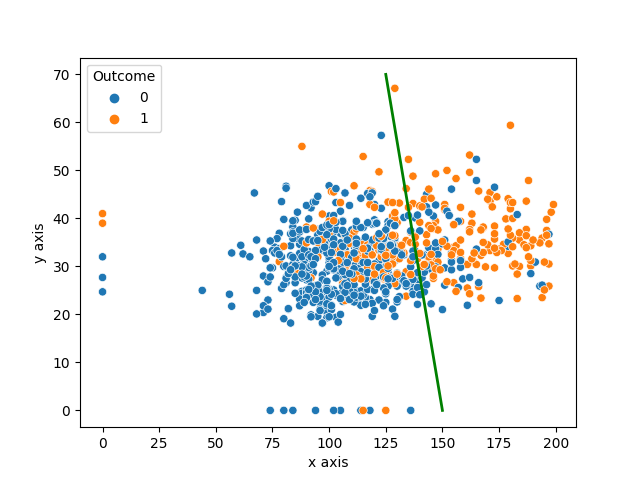
\includegraphics[trim=0 0 0 25, scale=0.54]{classification}
    \caption*{Nota\normalfont. La recta de color verde representa el plano que separa los datos, entre aquellos que son verdadero con valor uno y falso con valor cero.}
    \vskip-4ex
    \label{fig:ejclasi}
\end{figure}

Este tipo de clasificación se utiliza para predecir una clase discreta o etiqueta que puede tener dos estados, pero si el problema lo requiere se puede utilizar clasificación multi-clase. La clasificación con múltiples clases a diferencia de la clasificación binaria, no tiene únicamente los estados esperado y no esperado, sino que las salidas son clasificadas en una de todas las clases disponibles. 

Los modelos disponibles para Clasificación en Python a través de la librería scikit-learn \parencite{sklearn_api} que se utilizan en este proyecto son:

\begin{APAitemize}
    \item SVC rbf: La implementación de este estimador esta basada en libsvm con kernel igual a \textit{rbf}. El tiempo de entrenamiento se incrementa hasta el orden cuadrático cuando el número de muestras supera las diez mil unidades, por lo tanto es recomendable usar otras opciones si se presenta tal situación.
    \item LinearSVC: Similar a SVC con kernel igual a \textit{linear}, pero implementado en términos de liblinear en vez de lbsvm, por ende adquiere más flexibilidad en la selección de penalizaciones y pérdidas de función, con lo que tiene la posibilidad de escalar mejor para grandes cantidades de muestras.
    \item KNN: \textit{K Nearest Neighbours} Es un algoritmo que almacena los casos disponibles y realiza la clasificación de nuevos casos apoyándose en una medición de similaridad con base a la distancia \textit{k} entre una muestra y la otra.
    \item Gaussian Naive Bayes: Este estimador hace parte de los métodos Naive Bayes. Estos algoritmos están basados en la implementación de teorema de Bayes con la suposición de una independencia condicional entre las características, y de igual forma el algoritmo de clasificación Naive Bayes Gaussiana supone que la probabilidad de las características es Gaussiana.
\end{APAitemize}

\paragraph{Regresión} En este tipo de predicción el resultado se calcula a partir de un modelo que minimice la función de pérdida. Dado que la salida de estos algoritmos es un número, la Regresión (ver Figura ~\ref{fig:ejregre}) puede ser empleada tanto en problemas para clasificar clases, como estimar cantidad numéricas. Por tal motivo, es utilizada para predecir todo tipo de situaciones donde la salida sean datos continuos, por ejemplo: el valor de un seguro de vida y el valor en bolsa. 

\begin{figure}[H]
    \centering
    \caption{Ejemplo de Regresión}
    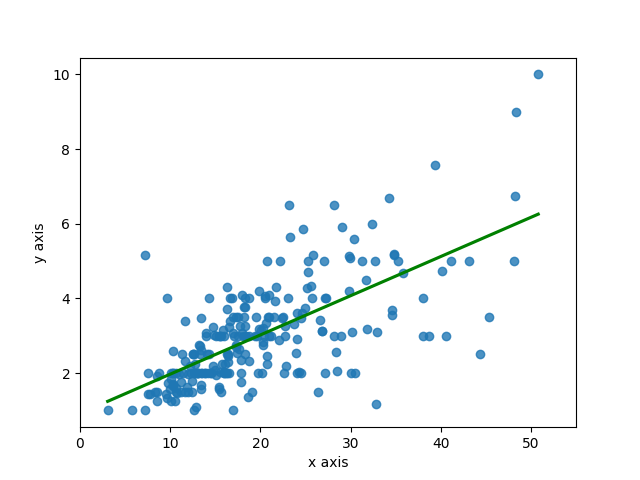
\includegraphics[trim=0 0 0 25,scale=0.5]{regression}
    \caption*{Nota\normalfont. La recta de color verde representa el comportamiento medio de los datos a partir de la función $f(x) = m\cdot x+b$ donde \textit{m} es la pendiente y \textit{b} el punto de corte con la abscisa.}
    \vskip-4ex
    \label{fig:ejregre}
\end{figure}

Los modelos disponibles de Regresión en Python a través de la librería scikit-learn \parencite{sklearn_api} que se utilizan en este proyecto son:

\begin{APAitemize}
    \item Lasso: Es un tipo de regresión lineal que utiliza contracción de los valores con base a un punto central, al igual que la media. Este procedimiento fomenta modelos más simples y dispersos, lo cual se traduce a modelos con menos parámetros.
    \item SGDClassifer: Este estimador implementa modelos lineales regulados, con un gradiente aleatorio de aprendizaje en descenso. El gradiente de las pérdidas se estima en cada muestra a la vez que modelo se actualiza en paraleo con la curva de aprendizaje.
    \item SVR rbf: Los parámetros en el modelo son \textit{C} y \textit{epsilon}. La implementación es basada en libsvm con kernel igual a \textit{rbf}. El tiempo de entrenamiento supera el orden cuadrático, de manera que es difícil trabajar con este modelo cuando el número de muestras supera las diez mil unidades.
    \item LinearSVR: Similar a SVC con kernel igual a \textit{linear}, pero implementado en términos de liblinear en vez de lbsvm. Permite mayor flexibilidad en la selección de penalizaciones y perdidas de función, y además escala mejor para grandes cantidades de muestras.
\end{APAitemize}

\paragraph{Agrupamiento} A este tipo de algoritmos se les conoce en inglés como \textit{Clustering} (ver Figura ~\ref{fig:ejcluster}). Su principal objetivo es entrenar un algoritmo para generar las agrupaciones deseadas, dado un conjunto de datos con sus respectivos datos históricos. La similitud de los grupos está dada por información adicional suministrada por el usuario, lo que puede convertirse en un problema de optimización de hiperparámetros, sobre todo si hay muchos atributos que deben considerarse para el entrenamiento. 

\begin{figure}[H]
    \centering
    \caption{Ejemplo de Agrupamiento}
    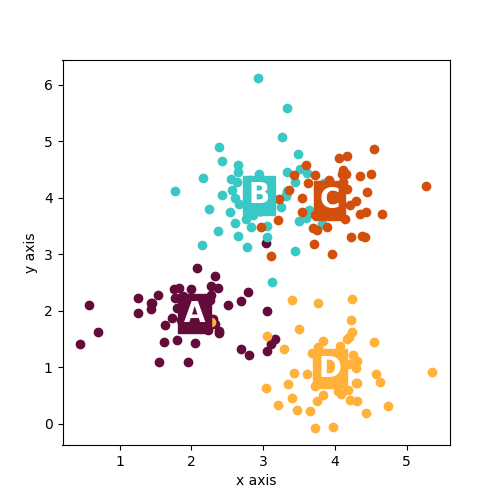
\includegraphics[trim=0 0 0 25,scale=0.5]{cluster}
    \caption*{Nota\normalfont. Cada \textit{cluster} está separado según su color. En este ejemplo, los grupos que se quieren predecir son A, B, C y D.}
    \vskip-4ex
    \label{fig:ejcluster}
\end{figure}

Los modelos disponibles de Agrupamiento en Python a través de la librería scikit-learn \parencite{sklearn_api} que se utilizan en este proyecto son:

\begin{APAitemize}
    \item Affinity Propagation: crea grupos a través del envío de mensajes entre las parejas en las muestras hasta que se haya convergencia. Un conjunto de datos es luego descrito utilizando una parte de las muestras, las cuales son seleccionadas como las más representativas entre el conjunto total de muestras.
    \item Kmeans: Este algoritmo agrupa información tratando de separar muestras en un numero de grupos equivalente a la varianza, minimizando un criterio conocido como la inercia o suma de los cuadrados dentro de un grupo. Este algoritmo requiere un número de grupos especificados desde el inicio, pero trabaja bien para un gran número de muestras, a diferencia de otros modelos.
    \item Minibatch Kmeans: Este algoritmo es una variante del algoritmo KMeans, el cual utiliza minilotes para reducir el tiempo de compilación, mientras optimiza la función objetivo.
    \item Meanshift: Esta forma de agrupamiento tiene como fin descubrir irregularidades en una superficie de muestras. Este algoritmo está basado en datos centrales llamados centroides, los cuales funcionan convirtiendo los candidatos en la media de los puntos dentro de una determinada región. Estos candidatos son filtrados en una etapa de post-procesamiento con la finalidad de eliminar cualquier duplicado cercano del conjunto de centroides finales.
\end{APAitemize}

\subsubsection{Selección de hiperparámetros}
\textcite{Wu2019} en su artículo \enquote{\textit{Hyperparameter optimization for machine learning models based on Bayesian optimization}} mencionan que los hiperparámetros son de gran importancia en el Aprendizaje de Máquina, dado que se encargan de cambiar el comportamiento de los algoritmos cuando entrenan el modelo. Por lo tanto, los hiperparámetros tienen una relación directa en el rendimiento final de cualquier modelo de Aprendizaje de Máquina, y no deben ser establecidos en valores arbitrarios, sino que deben ser valores obtenidos de algoritmos tales como búsqueda Exhaustiva o Bayesiana.

\paragraph{Búsqueda exhaustiva} Este tipo de búsqueda es conocida como en inglés como \textit{greedy}. La búsqueda Exhaustiva implica realizar una exploración utilizando todos los valores posibles dada una lista de elementos $S$, pero en la mayoría de casos no se busca optimizar un solo hiperparámetro, sino que se requiere realizar una búsqueda para al menos dos o más listas de valores. Esto da como resultado tiempos de ejecución polinómicos, es decir $O(n^k)$ donde \textit{k} es el número de listas de valores o espacios de parámetros y \textit{n} la cantidad de elementos en el espacio $S$, si todos las listas tienen la misma longitud.

Este algoritmo se encuentra disponible en la librería scikit-learn \parencite{sklearn_api} para Python, con dos diferentes opciones: GridSearchCV y RandomSearchCV. La opción elegida para este proyecto es GridSearchCV (ver Figura ~\ref{fig:impbusexh}), dado que esta puede realizar una búsqueda exhaustiva con todo el espacio de valores, a diferencia de RandomSearchCV que escoge un subconjunto del espacio de valores con respecto a una semilla aleatoria.

\begin{figure}[H]
    \centering
    \caption{Implementación de Búsqueda Exhaustiva}
    \inputminted{Python}{pycode/gridsearch.py}
    \label{fig:impbusexh}
\end{figure}

\paragraph{Búsqueda Bayesiana}  Este algoritmo está basado en el teorema de Bayes y se le conoce como búsqueda Bayesiana. A diferencia de una búsqueda Exhaustiva, es una de las estrategias más eficientes con respecto al número de evaluaciones necesarias. Esta búsqueda es utilizada comúnmente cuando las ya mencionadas evaluaciones requieren de grandes cantidades de tiempo, cuando el problema no es convexo y cuando no se tiene una expresión para la función objetivo, pero si se puede obtener la información de los eventos de la función \parencite{Brochu2010}. 

Este algoritmo se encuentra disponible en la librería scikit-learn \parencite{sklearn_api} para Python con el nombre de BayesSearchCV (ver Figura ~\ref{fig:impbusbay}), y aunque existan otras opciones de vanguardia, utilizar directamente la implementación de scikit-learn beneficia al proyecto en el tiempo de desarrollo requerido para desplegar la aplicación.

\begin{figure}[H]
    \centering
    \caption{Implementación de Búsqueda Bayesiana}
    \inputminted{Python}{pycode/bayesiansearch.py}
    \label{fig:impbusbay}
\end{figure}


\subsubsection{Reducción de dimensionalidad}
Existe la creencia respecto al volumen de los datos que más información es mejor, y por lo general es cierto, pero no en todos los casos esto se cumple. Un mayor número de observaciones redunda en un mejor modelo, pero un mayor número de variables no necesariamente lo hace mejor \parencite{Guerrero2016}. Para conjuntos de datos con varias dimensiones, la reducción de dimensionalidad se ejecuta antes de aplicar los algoritmos de Aprendizaje de Máquina, con el propósito de evitar los problemas relacionados a la maldición de la dimensionalidad. Por tales motivos, autores en años anteriores como \textcite{Finley2005} mencionan que la selección de características se convierte en la opción mas viable, especialmente en conjuntos de datos con alta dimensionalidad.

Existen diferentes tipos de métodos con los cuales se aborda el problema de la reducción de la dimensionalidad, sin embargo, de acuerdo con \textcite{Finley2005,Sanchez-Marono2007} los más utilizados son los métodos de filtrado y envolventes. Estos métodos pretenden hallar un subconjunto de datos a partir del original, es decir, que el nuevo subconjunto candidato a ser la opción óptima pierde una o más características en el proceso. Esto da como resultado en el mejor de los casos un incremento en el rendimiento del clasificador, mientras que por otro lado, si el proceso de selección de características no es necesario desde el inicio, el resultado final es un clasificador con un rendimiento menor al inicial, dado que las características eliminadas eran significativas. 
 
\paragraph{Métodos de filtrado} Los métodos de filtrado realizan un análisis de las características individuales para identificar su importancia relativa. Son computacionalmente eficaces e independientes del modelo, pero por otro lado, es posible que una característica no sea útil por si sola, aunque puede ser significativa cuando está asociada con otra. Esta situación representa una desventaja en los métodos de filtrado, ya que se puede perder la potencial importancia de dichas características. 

Los algoritmos disponibles para métodos de filtrado en Python a través de la librería scikit-learn \parencite{sklearn_api} son:
 
 \begin{APAitemize}
     \item VarianceThreshold: es un método para la selección de características que remueve toda aquella característica cuya varianza no supere cierto límite. Adicionalmente, por defecto elimina toda característica con varianza cero, es decir aquellas que tienen el mismo valor en todas las muestras y por ende no otorgan información relevante.
     \item SelectKBest: este algoritmo se encarga de remover todas las características que no pertenezcan a las \textit{k} características con mayor peso. La salida puede ser un nuevo vector con las nuevas características o el peso individual de cada una de ellas.
     \item SelectPercentile: es un algoritmo que remueve toda característica que el usuario no seleccione entre las de mayor puntuación.
     \item GenericUnivariateSelect: este algoritmo utiliza una estrategia configurable para realizar una selección de características univariadas.
 \end{APAitemize}
 
\paragraph{Métodos envolventes} Este tipo de métodos inician el proceso de evaluación de las características una a una, para luego seleccionar aquella que tiene el mejor rendimiento. Una vez terminado ese proceso se realiza la selección de las posibles combinaciones hasta que el modelo no tenga un mejor rendimiento con respecto a la última iteración. 
 
Los algoritmos disponibles para métodos envolventes en Python a través de la librería scikit-learn \parencite{sklearn_api} son:
 
 \begin{APAitemize}
     \item Recursive Feature Elimination: el objetivo de este método es la eliminación de características generando un conjunto de características cada vez más pequeño. Las características menos importantes son eliminadas del conjunto de características actuales, proceso que se repite constantemente hasta llegar a la cantidad requerida de características
     \item SelectFromModel: este algoritmo puede ser utilizado con cualquier estimador que tenga los atributos coeficiente o importancia de característica, después de realizar el entrenamiento del modelo. Las características por defecto son consideradas no relevantes al no superar el umbral suministrado, mientras que aquellas que califican como importantes se mantienen.
     \item Sequential Feature Selector: es un algoritmo exhaustivo que se utiliza para reducir el espacio de características de cierta dimensionalidad a un espacio de menor dimensionalidad. Tiene como finalidad seleccionar automáticamente un subconjunto de características que son relevantes para el problema. 
     \item Exhaustive Feature Selector: este algoritmo evalúa subconjuntos de características exhaustivamente aplicando todas las posibles combinaciones. El mejor subconjunto se selecciona a partir del rendimiento obtenido entre todas las iteraciones con el modelo seleccionado, ya sea Regresión o Clasificación.
 \end{APAitemize}
 
\subsubsection{Aprendizaje automático}
Inicialmente todos los procesos de Aprendizaje de Máquina se realizaban paso a paso, pero con el desarrollo del primer algoritmo automatizado por parte de \textcite{Thornton2013} en su trabajo titulado ``\textit{Auto-Weka}'' el panorama cambia a uno donde es más efectivo utilizar algoritmos de aprendizaje automático para problemas de nivel empresarial. La ruta más fácil para seleccionar un estimador utilizada por estudiantes es definida a partir de la popularidad que tenga o que tan sencillo parece de utilizar, por consiguiente no se consideran las alternativas disponibles que pueden ser más eficientes. Parte de esos inconvenientes son remediados con los repositorios de acceso libre desarrollados para el uso de la comunidad, tales como: Weka \parencite{Hall2009}, scikit-learn \parencite{scikit-learn} y mljar-supervised \parencite{mljar2018}, los cuales ofrecen paquetes de selección de características, hiperparámetros y modelo por medio de sus algoritmos de aprendizaje automático.

En trabajos posteriores \textcite{Feurer2020} en su artículo ``\textit{Auto-Sklearn 2.0: The Next Generation}'' mencionan que a partir de mejoras en su algoritmo original de Auto-sklearn, obtienen mejoras significativas a partir de la implementación de una técnica de meta-aprendizaje más sencilla, la cual según los autores es el futuro para tener un Aprendizaje de Máquina automatizado cercano a la perfección y que además sea de libre acceso. No obstante, implementar esta librería actualmente no es posible dado que aún se encuentra en desarrollo, y pese a que la versión 1.0 se encuentra disponible desde el año 2016, es únicamente para sistemas operativos Linux. Por tales motivos, la librería utilizada para cubrir las funcionalidades de aprendizaje automático en el presente proyecto es mljar-supervised (ver Figura ~\ref{fig:impautoml}), la cual es desarrollada por \textcite{mljar2018} como un proyecto de software libre. Esta librería al igual que otros algoritmos de aprendizaje automatizado, tiene las funcionalidades de vanguardia necesarias para ejecutar optimización de hiperparámetros y selección de modelo, dado que si es necesario, los usuarios de \textit{Voorspelling} pueden elegir entre un proceso paso a paso o automático; decisión que está relacionada al objetivo del proyecto.

\begin{figure}[H]
    \centering
    \caption{Implementación de AutoML}
    \inputminted{Python}{pycode/automl.py}
    \label{fig:impautoml}
\end{figure}

\subsection{Desarrollo de aplicaciones}
\subsubsection{Definición}
El estudio o disciplina que comprende crear aplicaciones de software confiables y de calidad a través de etapas sistematizadas se conoce en el área de las ciencias de la computación como Ingeniería de Software \parencite{Sommerville2005}. Una aplicación o también conocida como \textit{app}, de acuerdo con \textcite{Pressman2002} es un tipo de software desarrollado con la función de ayudar al usuario en la realización de tareas determinadas y como la mayoría de las aplicaciones, estas son resultado de satisfacer una necesidad específica que desencadena una oportunidad de negocio. Su tamaño puede comprender desde códigos no muy extensos de funciones muy especializadas, hasta grandes obras de la ingeniería informática que toman un gran personal y muchas horas de trabajo para ser desarrolladas.

Las tareas realizadas por las aplicaciones abarcan un campo extenso que no se limita a áreas de la informática, aun así desarrollar una aplicación es labor de un programador o una compañía de Software, es decir, un software se crea por un especialista informático conocido como desarrollador, que por medio de herramientas como software y lenguajes de programación crea una aplicación la cual satisface unos requerimientos preestablecidos. 

\subsubsection{Tipos de aplicaciones}
Las aplicaciones surgen de una de las ramas de los programas informáticos que se conocen como software. Aunque se pueden categorizar de muchas maneras tal como lo menciona \parencite{Pressman2002}, se conoce que de acuerdo con sus fines prácticos se puede clasificar como:

\begin{APAitemize}
    \item Software de sistema: rigen el comportamiento del sistema. Usualmente genera una separación entre el usuario y los componentes que conforman el ordenador. 
    \item Software de aplicación: son programas informáticos hechos para desarrollar determinadas tareas. Su utilidad radica en la automatización o asistencia en procesos.
    \item Software de programación: este tipo de software es usado para desarrollar o modificar programas informáticos por medio de lenguajes de programación como Java, C++, C, C\#, Ruby, Go, Fortran y Python.
\end{APAitemize}

\subsubsection{Normas}
% La RAE \parencite{RAEDefNorma} define las normas como un conjunto de reglas que se debe seguir o a que se deben ajustar las conductas, tareas y actividades.
En el desarrollo de aplicaciones las normas conforman unos estándares los cuales rigen el curso a tomar por los proyectos de software. Por tal motivo, la aplicación de las normas tiene como objetivo que el software desarrollado ofrezca una mayor confiabilidad, mantenibilidad, usabilidad, productividad y calidad. 

Las normas de las cuales se abstrae los lineamientos para desarrollar software de calidad en el presente proyecto son:

\begin{APAitemize}
    \item ISO/IEC 11581-10:2010: aporta una guía a los desarrollares y diseñadores para crear o usar iconos con base a los estándares de iconografía \parencite{Iso11581}. Por otro lado, esta norma brinda una linea base para crear nuevas partes relacionadas a los iconos de un proyecto, dado que estos elementos no son solo símbolos, sino que son un medio para lograr un objetivo en una aplicación.
    \item ISO 9241-112:2017: aporta principios sobre la presentación de información en las interfaces de usuario. Al aplicar este principio se buscan interfaces más entendibles, precisas y  más rápidas, debido a la reducción de esfuerzo mental y una mejor experiencia de usuario \parencite{Iso9241-112}. En pocas palabras, es un estándar de usabilidad para no generar ambigüedades en el entendimiento de la información consecuente y extensa.
    \item ISO 9241-210:2019: aporta requerimientos y recomendaciones para los principios de diseño centrados en el ser humano, así como las actividades del ciclo de vida de sistemas interactivos basados en computadores \parencite{Iso9241-210}. Esta norma está diseñada para ser utilizada por aquellos que gestionan el proceso de diseño de \textit{software}, pero de igual forma está relacionada con las formas en que el \textit{hardware} y \textit{software} de sistemas interactivos pueden optimizar la interacción humano-máquina.
\end{APAitemize}

Por otro lado, dado que el lenguaje de programación principal de la aplicación de escritorio es Python, los estándares que utilizan los desarrolladores para generar código de calidad son: PEP8, PEP20, PEP257, PEP3131, PEP 484 y PEP 526.

\begin{APAitemize}
    \item PEP8: es una guía para generar código en Python comprensible para todo desarrollador. La guía tiene como finalidad mejorar la legibilidad del código, hacerlo consistente y más coherente \parencite{PEP8Python}. La herramienta de autoPEP8 disponible en todo editor de texto utiliza pycodestyle para seleccionar que partes del código debe de ser reorganizados acorde al estilo de PEP8. Por lo tanto, no es necesario indagar profundamente si un archivo cumple o no con el estándar, dado que el proceso es automatizado. 
    \item PEP20: este estándar es la guía de principios BDFL para diseño en Python en 20 aforismos. Algunos de estos son: Explicito es mejor que implícito, plano es mejor que anidado, la legibilidad cuenta, los errores nunca deben pasar desapercibidos, y si la implementación es fácil de explicar, entonces puede que sea una buena idea \parencite{PEP20Python}. 
    \item PEP257: su objetivo es estandarizar la estructura de los comentarios de documentación en métodos, funciones y clases, es decir, qué deberían contener y cómo lo expresan \parencite{PEP257Python}.
    \item PEP3131: este estándar expone que todos los identificadores en la biblioteca estándar de Python deben usar palabras en Inglés en formato ASCII \parencite{PEP3131Python}. Adicionalmente los comentarios deben ir también en ASCII, aunque hay un par de excepciones: los casos de prueba y nombres propios.
    \item PEP484: este estándar tiene como objetivo establecer la sintaxis para las anotaciones, posibilitando que el código de Python sea más fácil de analizar, refactorizar y en algunos casos generar código a partir de realizar validación del tipo de variable. \parencite{PEP484Python}.
    \item PEP526: en este estándar el tema principal son las anotaciones de variables. Según la documentación \parencite{PEP526Python} las notaciones para variables a nivel de módulo, clase, instancias y variables locales deben de tener un espaciado simple después de las comas y dos puntos, situación que es similar con los símbolos de igualdad, aunque en ese caso si hay espaciado antes y después. 
\end{APAitemize}

\subsubsection{Documentación}
En el contexto del software, la documentación consiste en explicar cómo está compuesta y organizada una aplicación, siendo necesaria para generar el entendimiento del sistema de quienes lo vayan a usar y mantener. La documentación en muchos casos depende de los procesos de la organización donde se desarrolla, pero aquellas que utilizan buenas prácticas seguramente respetan el sistema por medio del lenguaje de modelado unificado (UML), el cual brinda diagramas estandarizados, siendo los diagramas de caso de uso y clase los más frecuentemente aplicados, ya que aportan significativamente al entendimiento de la arquitectura del sistema \parencite{Rumbaugh2004}. Aunque dependiendo del problema se pueden utilizar otros diagramas UML, tales como: secuencia, componentes, actividades y estado. 
En el presente proyecto los diagramas que se utilizan para describir el sistema y sus interacciones son el diagrama de casos de uso, clase y actividades.

\paragraph{Diagramas de caso de uso} Se utilizan para capturar el dinamismo de un sistema y busca plasmar los requisitos del sistema en un diseño de alto nivel, dado que idealizan la ruta del usuario al interactuar con el sistema. Este tipo de diagrama representa el conjunto de funcionalidades del sistema y el flujo que toma hasta llegar a un resultado. Sin embargo, los comportamientos en el diagrama de casos de uso tienden a ser de alto nivel y no se menciona la estructura lógica interna de estos. 

\paragraph{Diagramas de clase} Estos diagramas describen los objetos en un sistema, mostrando los atributos y métodos que los componen, y adicionalmente las relaciones entre los objetos. Estos diagramas representan el sistema de una forma estática, por ende, no describe como se comportan los distintos elementos a lo largo de la ejecución, aun así son útiles, ya que son aplicables tanto para sistemas pequeños como grandes, y gracias a sus propiedades se transforma cómodamente el modelo a código fuente.

\paragraph{Diagramas de actividades} Descomponen las actividades y se utilizan para hacer un modelado de alto nivel de los requisitos. A este tipo de diagrama se les consideran diagramas de comportamientos ya que muestran el sistema de una manera dinámica junto a sus relaciones, por lo tanto, son similares a los diagramas de flujo (DFD), aunque tiene sutiles diferencias. El diagrama de actividades plantea un flujo de trabajo con un principio y un fin definidos, el cual puede desenvolverse como un flujo único, paralelo, concurrente o de acuerdo con la necesidad. Estos diagramas son utilizados para representar la lógica interna de los algoritmos que componen el sistema, especialmente los casos de uso.

Los formatos utilizados en la documentación del proyecto son una representación simplificada de la norma técnica colombiana, conservando sus principales características técnicas y enfocándose en la información de mayor relevancia. Los más importantes utilizados en este proyecto son el formato de levantamiento de requerimientos, casos de uso, clases y pruebas.

\paragraph{Formato de levantamiento de requerimientos} Este formato está conformado por tres secciones: el encabezado donde se encuentra el nombre del autor, la fecha de creación, el propósito, alcance, características del usuario, entorno operativo y requerimientos mínimos del sistema. Después del encabezado se encuentra el cuerpo, el cual alberga la lista de los requerimientos funcionales y no funcionales. Cada uno de los elementos tiene su respectivo código, descripción, prioridad y requerimientos asociados. Por último, la aprobación que contiene el control de cambios y la firma del director del proyecto.

\paragraph{Formato de casos de uso} Este formato está conformado por tres secciones: el encabezado donde se encuentra el nombre del autor y la fecha de creación. Después de este se encuentra el cuerpo, el cual alberga el nombre del caso de uso, código, versión, módulo, actor, objetivo, descripción de escenario, flujo, resultados esperados, precondiciones, excepciones, postcondiciones y el diagrama correspondiente a dicho caso. Por último, la aprobación que contiene el control de cambios y la firma del director del proyecto.

\paragraph{Formato de clases} Este formato esta conformado  por tres secciones: el encabezado donde se encuentra el nombre del autor y la fecha de creación. Después se encuentra el cuerpo, el cual alberga el código asignado al diagrama, nombre del diagrama, descripción del escenario, las clases que conforman el diagrama con una casilla para cada tipo y el diagrama de clase respectivo. Por último, la sección de aprobación que contiene el control de cambios y la firma del director del proyecto.

\paragraph{Formato de pruebas} Este formato está conformado por tres secciones: el encabezado donde se encuentra el nombre del autor y la fecha de creación. Después de este se encuentra el cuerpo que alberga el objetivo de la prueba, las técnicas, el código involucrado, el caso de prueba (contiene un formato anidado) y observaciones. Por último la aprobación, la cual contiene el control de cambios y la firma del director del proyecto.

\subsubsection{Metodología de desarrollo}
La metodología de acuerdo con \textcite{CambridgeDefMethodology} se identifica como un conjunto de procedimientos sistemáticos, técnicas, enseñanza y estudio de un tema, que son utilizadas para el diseño, planificación y documentación de los sistemas de información. Si el tema principal es desarrollar software, la Ingeniería de Software toma el papel principal de aplicar una metodología, dividiendo el proyecto en secciones más pequeñas, planteando una serie de pasos o etapas, las actividades correspondientes del proyecto, y por último, las entradas y sus respectivas salidas \parencite{Sommerville2005}. El objetivo de las metodologías es exponer un conjunto de técnicas para modelar sistemas, dado que estas permiten desarrollar un software de calidad.

Cada tipo de metodología tiene su propio enfoque, fortalezas y debilidades, haciéndolas más factibles o endebles en determinados casos. Las metodologías ágiles combinan una filosofía y unos lineamientos de desarrollo, buscan ejecutar una serie de pasos para obtener la satisfacción del cliente, buenos tiempos de entrega, sencillez al ser desarrollado el software y una comunicación constante y activa con el cliente final \parencite{Pressman2002}. La correcta aplicación de una metodología genera un software que crece constante y rápidamente, y que además es exitoso, es decir, un software completamente operativo entregado en las fechas acordadas y que cumple con los requerimientos establecidos. Las metodologías ágiles se enfocan en diferentes aspectos del ciclo de vida del desarrollo de software y difieren una de otra por el enfoque que tienen. Algunas metodologías ágiles se enfocan en las buenas prácticas, por ejemplo, Programación Extrema (XP), mientras que otras se enfocan en la gestión de proyectos de software, como es el caso de Scrum, Kanban y Scrumban \parencite{Khan2014}.

\paragraph{Scrumb} Esta metodología incorpora un conjunto de patrones del proceso que realzan las prioridades del proyecto, las unidades de trabajo agrupadas, la comunicación y la retroalimentación frecuente con el cliente. En este modelo una organización se divide en pequeños equipos auto-organizados con tamaños que van de cuatro a diez personas, donde se consta de un propietario de producto, el equipo de desarrollo, \textit{testers} y un \textit{Scrum Master}. Un equipo de Scrum además de auto-organizado debe ser multifuncional y tener todas las competencias necesarias para realizar el proyecto sin la necesidad de intervención externa.

\paragraph{Kanban} Usando esta metodología el flujo de trabajo en el proyecto de desarrollo de software se visualiza usando un tablero llamado Kanban. El tablero Kanban tiene columnas que representan las etapas de trabajo, los hitos que se muestran como notas adhesivas y además en cada columna se puede especificar subcolumnas para tener un mayor orden de cada tarea. La metodología Kanban se basa en los principios de visualizar el flujo de trabajo del proceso, limitar el trabajo en curso y controlar el tiempo de entrega. Por tales motivos, es útil cuando se necesitan que los equipos conozcan el flujo de trabajo del proyecto, el estado actual de los hitos y que se realiza en el momento.

\paragraph{Scrumban} Es resultado de la combinación de los modelos de desarrollo Scrum y Kanban. Esta metodología intenta utilizar las mejores características de ambos modelos, usando la naturaleza descriptiva de Scrum para ser ágil y la mejora de procesos de Kanban para que el equipo mejore continuamente en el proceso. Una de las herramientas que adquiere principalmente de Kanban es visualizar el flujo de trabajo, debido a que el equipo puede visualizar cada una de las etapas, y por lo tanto, ayuda a conocer los encargados de las tareas y el estado actual del proyecto.

\paragraph{Programación Extrema} Esta metodología de desarrollo se centra en aplicar una clara comunicación y trabajo de equipo, que por lo general sucede entre dos personas. Es ligera e ideal para equipos pequeños y medianos que desarrollan software con requerimientos no muy bien definidos o que tienden a cambiar. Se distingue de otras metodologías por su confianza en la comunicación oral y como deben relacionarse las personas, interacciones sociales que según \textcite{Beck2004} se consideran en XP tan importantes como las habilidades técnicas.




\clearpage
\section{Desarrollo metodológico}
\input{chapters/metodología}

\clearpage
\section{Conclusiones}
El presente proyecto responde a la necesidad de herramientas académicas para iniciar a estudiantes de carreras a fines a las ciencias de la computación en aprendizaje de máquina supervisado, por medio de un software de escritorio para el sistema operativo Windows 10,  documentación detallada y la utilización de una interfaz de usuario que facilita el proceso de creación de modelos tanto automáticos como convencionales.

Voorspelling durante su desarrollo, como todo proyecto de software, requirió de cambios en sus requerimientos y diseño para adaptarse a las necesidades y problemas que se presentan durante un desarrollo de software. Esta aplicación como se menciona anteriormente no es la excepción, por tal motivo, incluso después de su primer lanzamiento oficial, requiere de mejoras y actualizaciones para obtener un producto que responda a las necesidades de sus usuarios.

El estado actual del software cumple con los requerimientos aceptados por el director de proyecto, se realizan mejoras constantes en el producto y hay una ruta trazada para las futuras actualizaciones, la cual identifica como prioridad la mejora de la interfaz gráfica, soporte para otros sistemas operativos e idiomas.

Toda la documentación y código fuente se encuentra disponible en el repositorio del proyecto desde Marzo del 2021 para que futuros grupos de desarrollo continúen o creen sus propias versiones a partir de la arquitectura existente, ya sea utilizando únicamente el \textit{back-end} de la aplicación o el sistema completo.
 


\clearpage
\printbibliography[{heading=bibintoc}]
\thispagestyle{otherplain}

\appendix

\section{Vista de rutas alternativas}
\begin{figure}[H]
    \centering
    \caption{Página: estimadores de clasificación}
    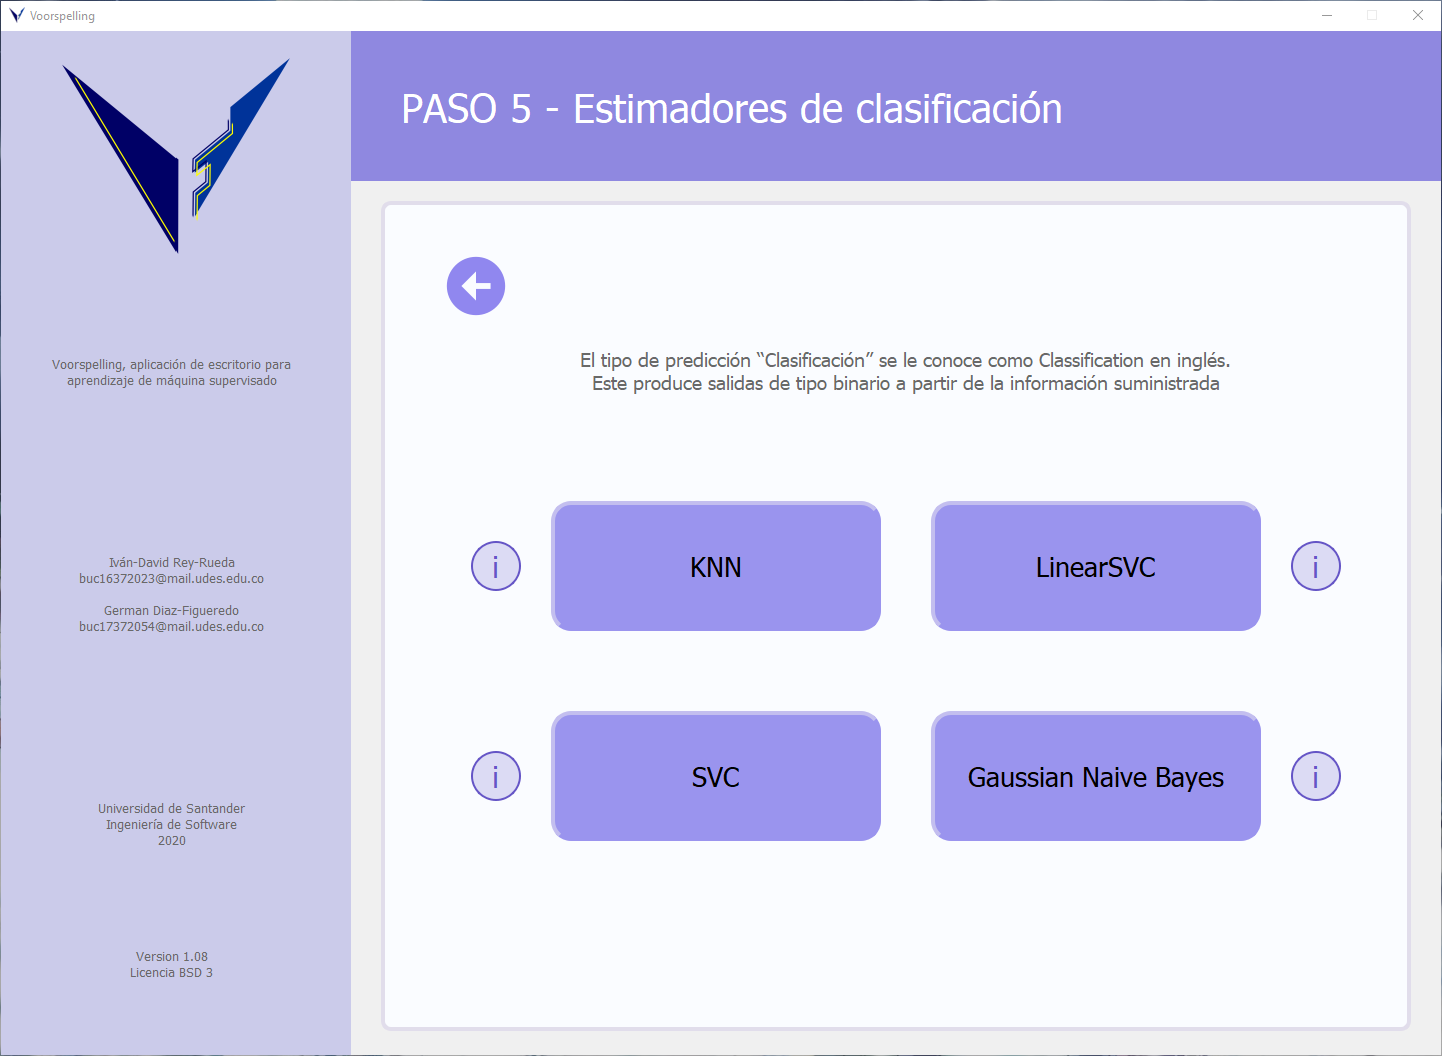
\includegraphics[width=\textwidth]{views/classification_estimators.png}
    \label{fig:classificationestimators}
\end{figure}

\begin{figure}[H]
    \centering
    \caption{Página: estimadores de regresión}
    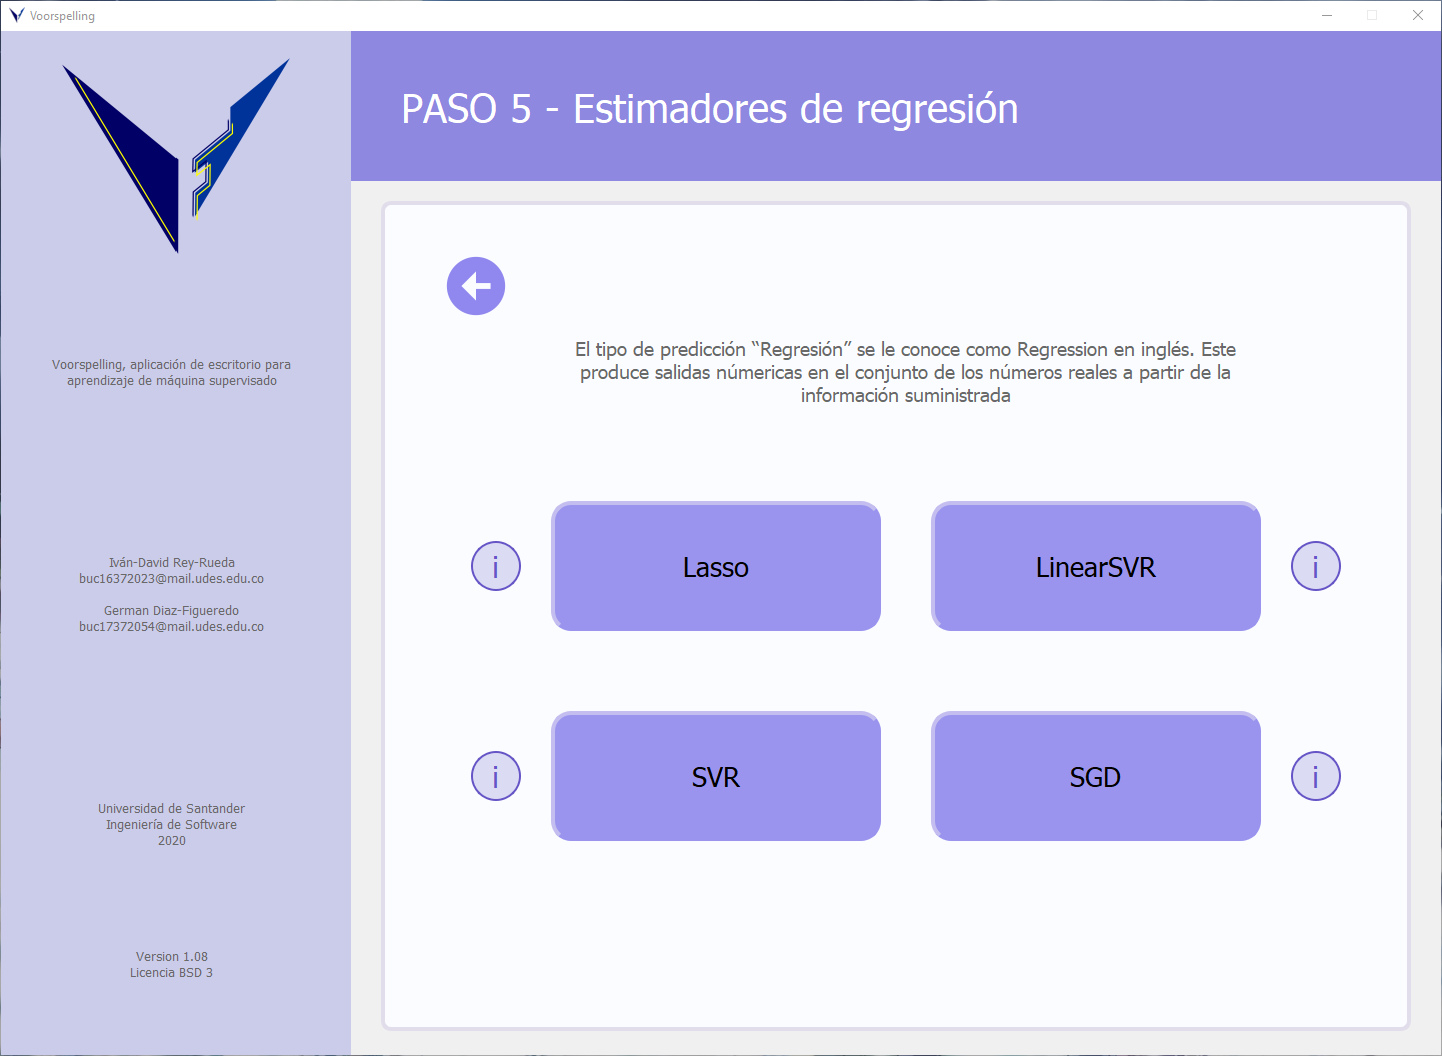
\includegraphics[width=\textwidth]{views/regression_estimators.png}
    \label{fig:regressionestimators}
\end{figure}

\begin{figure}[H]
    \centering
    \caption{Página: estimadores de agrupamiento}
    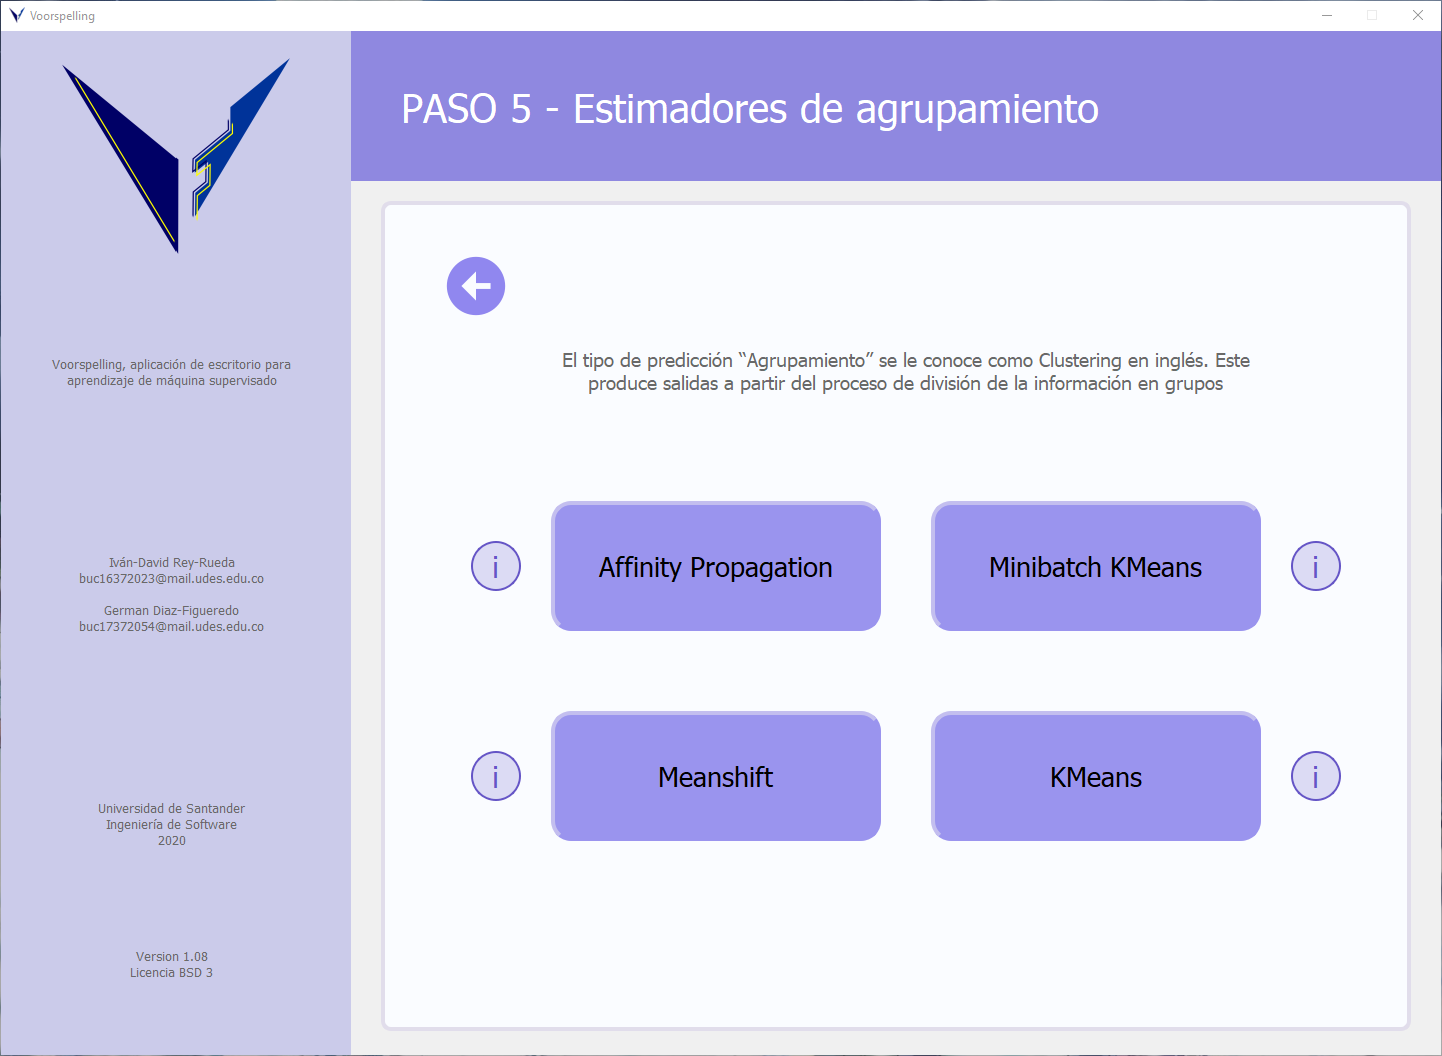
\includegraphics[width=\textwidth]{views/clustering_estimators.png}
    \label{fig:clusterestimators}
\end{figure}

\begin{figure}[H]
    \centering
    \caption{Página: método de selección de características}
    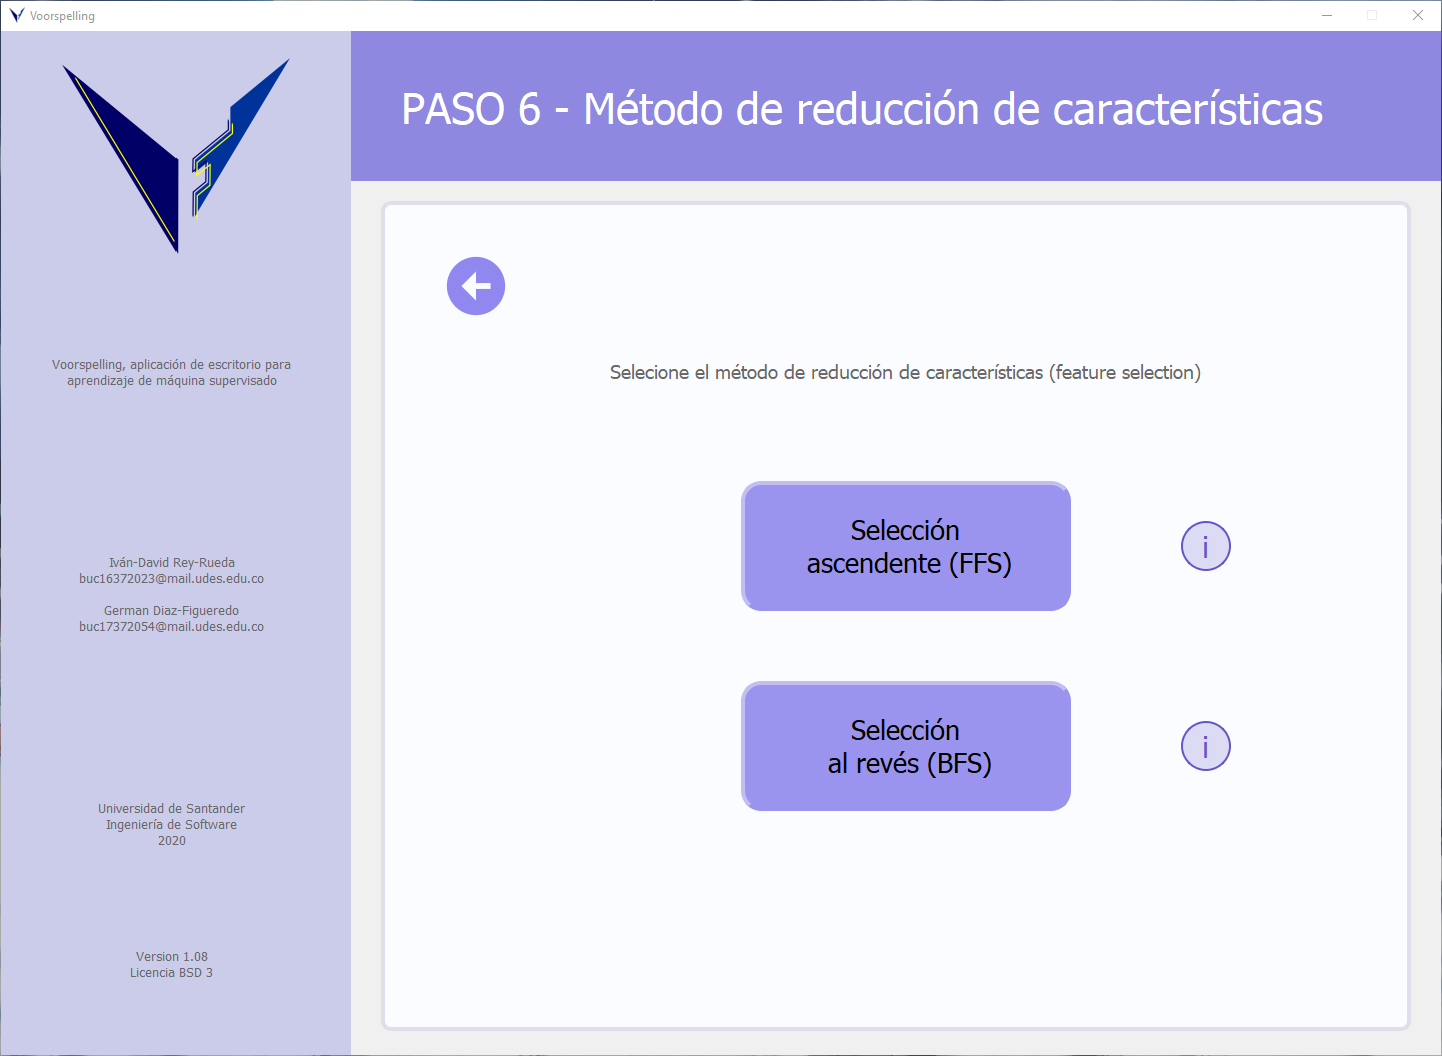
\includegraphics[width=\textwidth]{views/feature_selection_method.png}
    \label{fig:featureselectionmethod}
\end{figure}

\begin{figure}[H]
    \centering
    \caption{Página: método de búsqueda de hiperparámetros}
    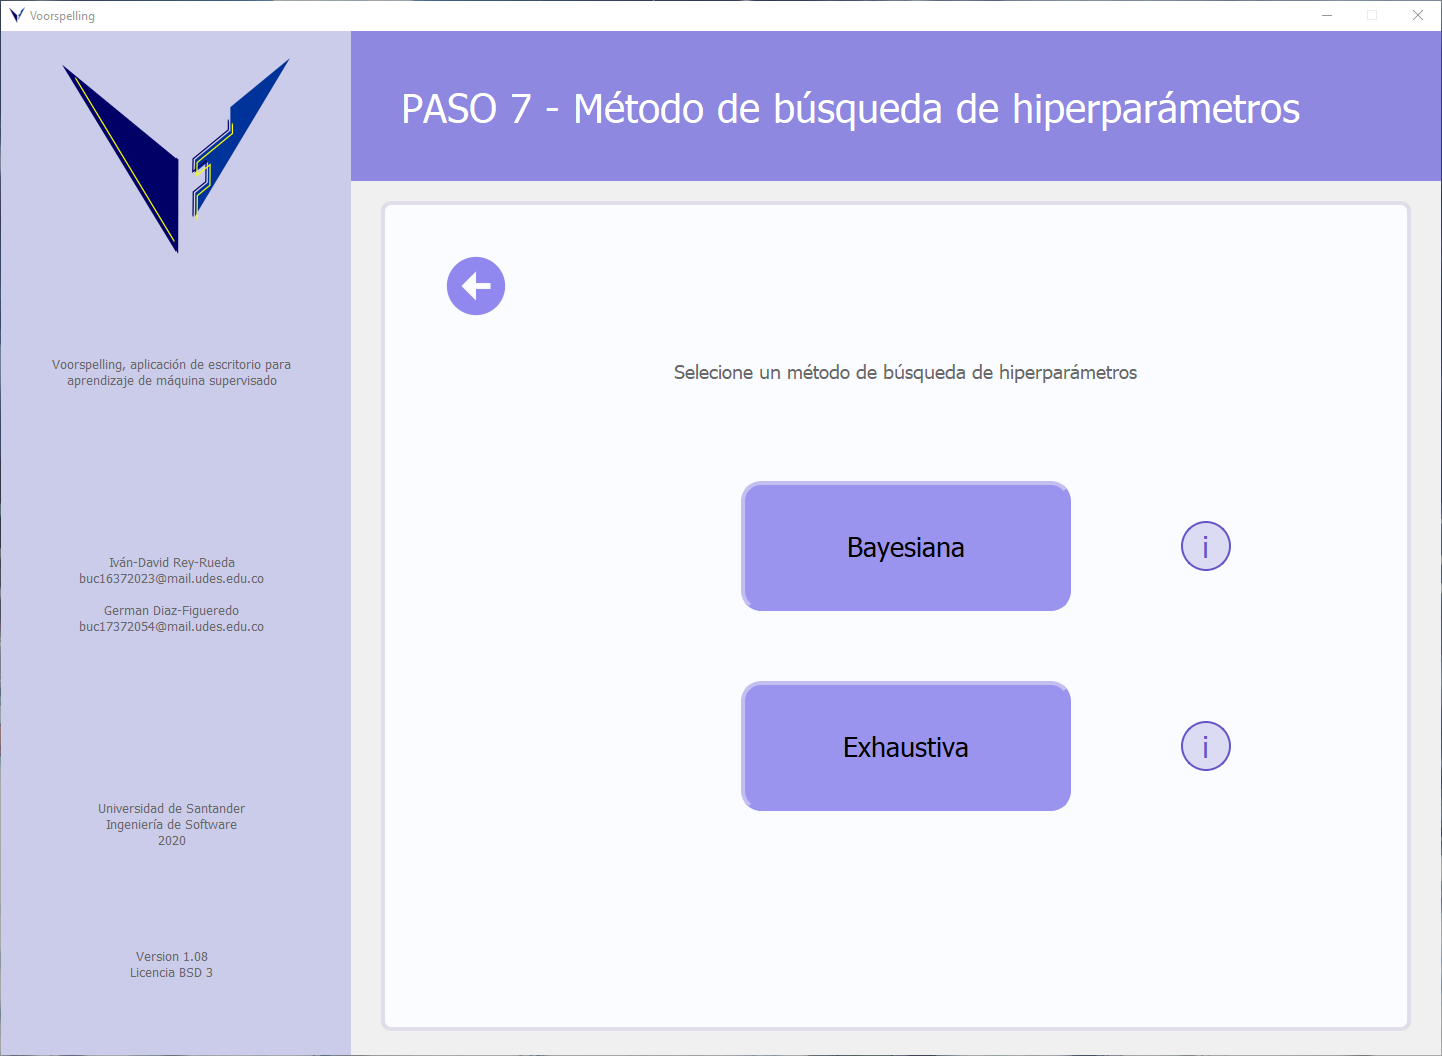
\includegraphics[width=\textwidth]{views/hiperparameter_search_method.png}
    \label{fig:hiperparamsearchmethod}
\end{figure}




\section{Vista para ingreso de hiperparámetros}
\begin{figure}[H]
    \centering
    \caption{Página: hiperparámetros de KNN}
    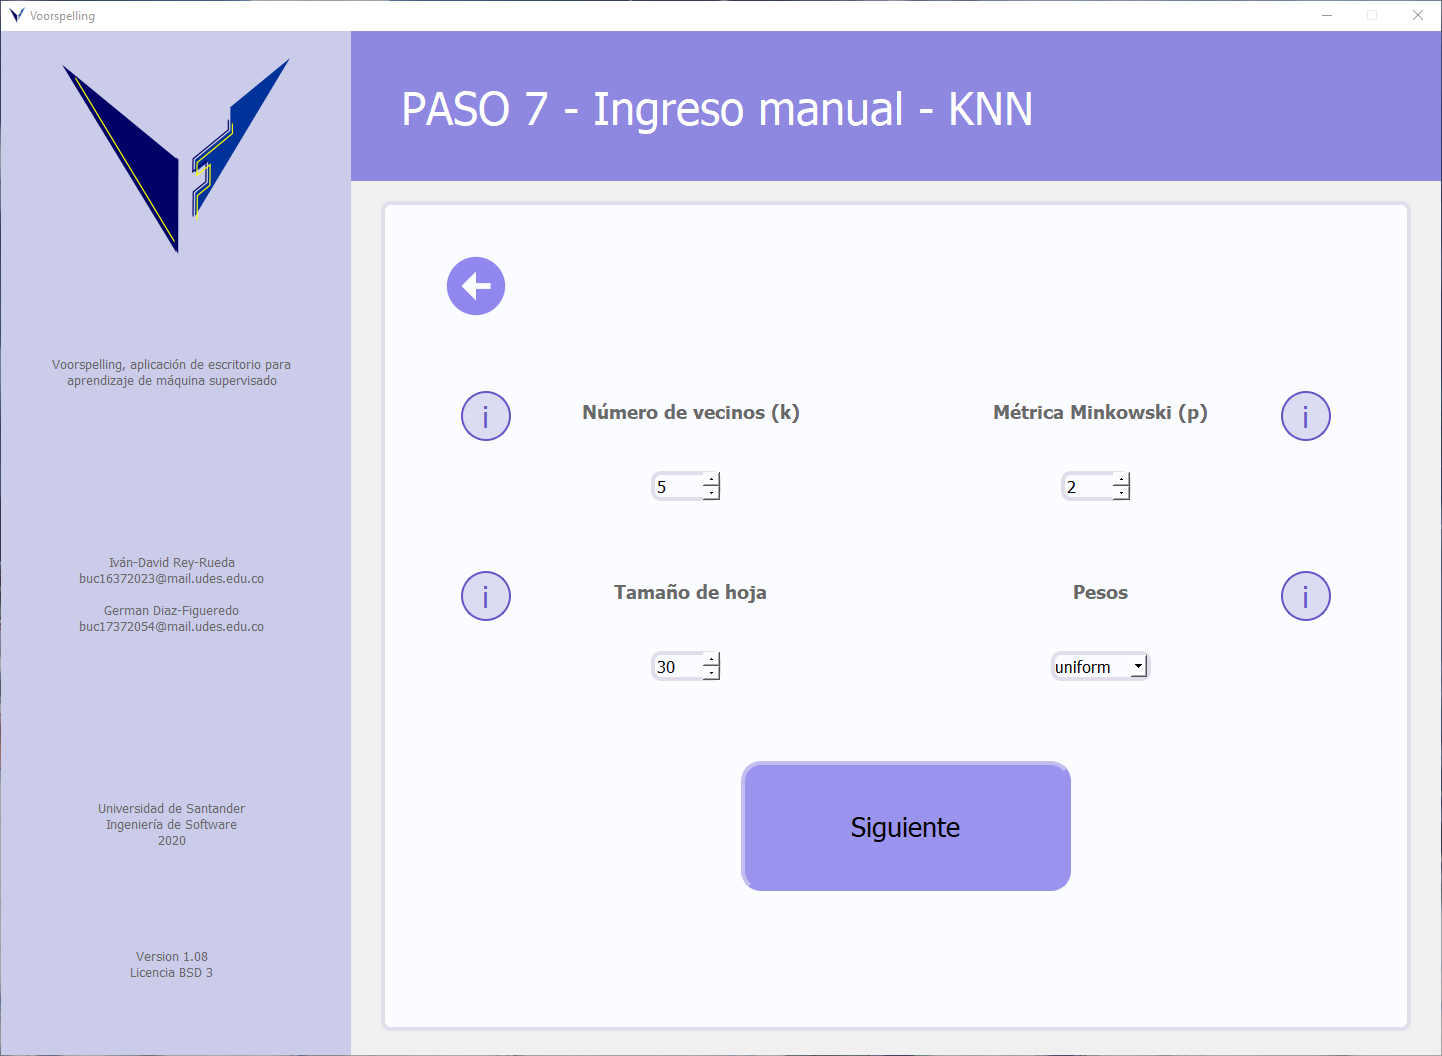
\includegraphics[width=\textwidth]{views/knn.png}
    \label{fig:knn}
\end{figure}

\begin{figure}[H]
    \centering
    \caption{Página: hiperparámetros de LinearSVC}
    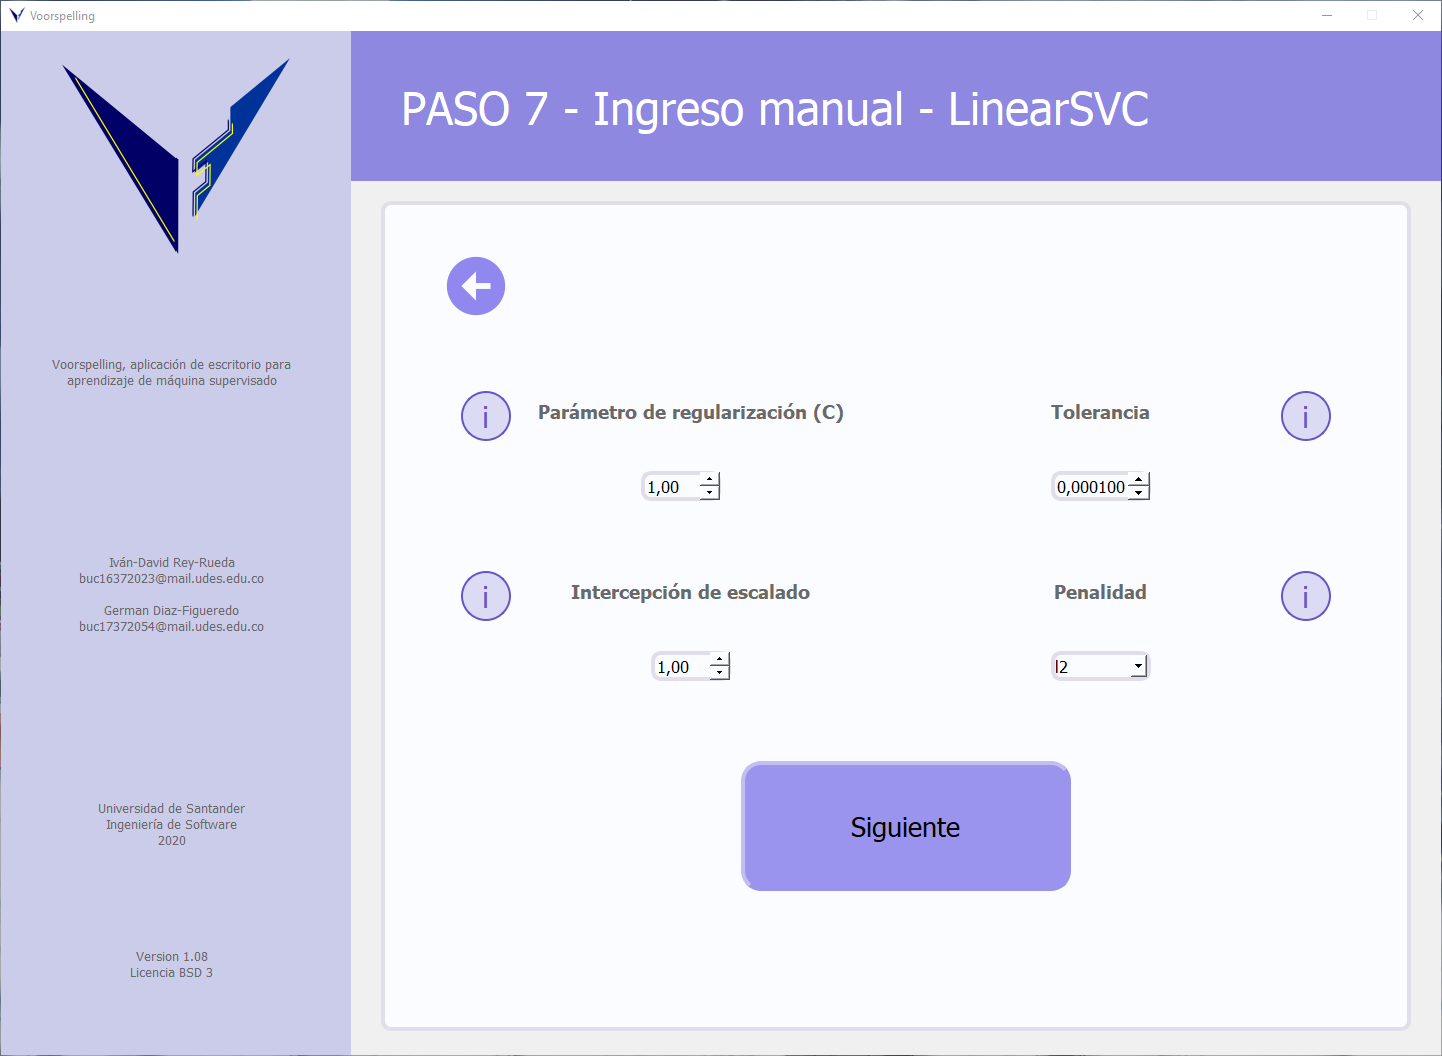
\includegraphics[width=\textwidth]{views/linearsvc.png}
    \label{fig:linearsvc}
\end{figure}

\begin{figure}[H]
    \centering
    \caption{Página: hiperparámetros de SVC}
    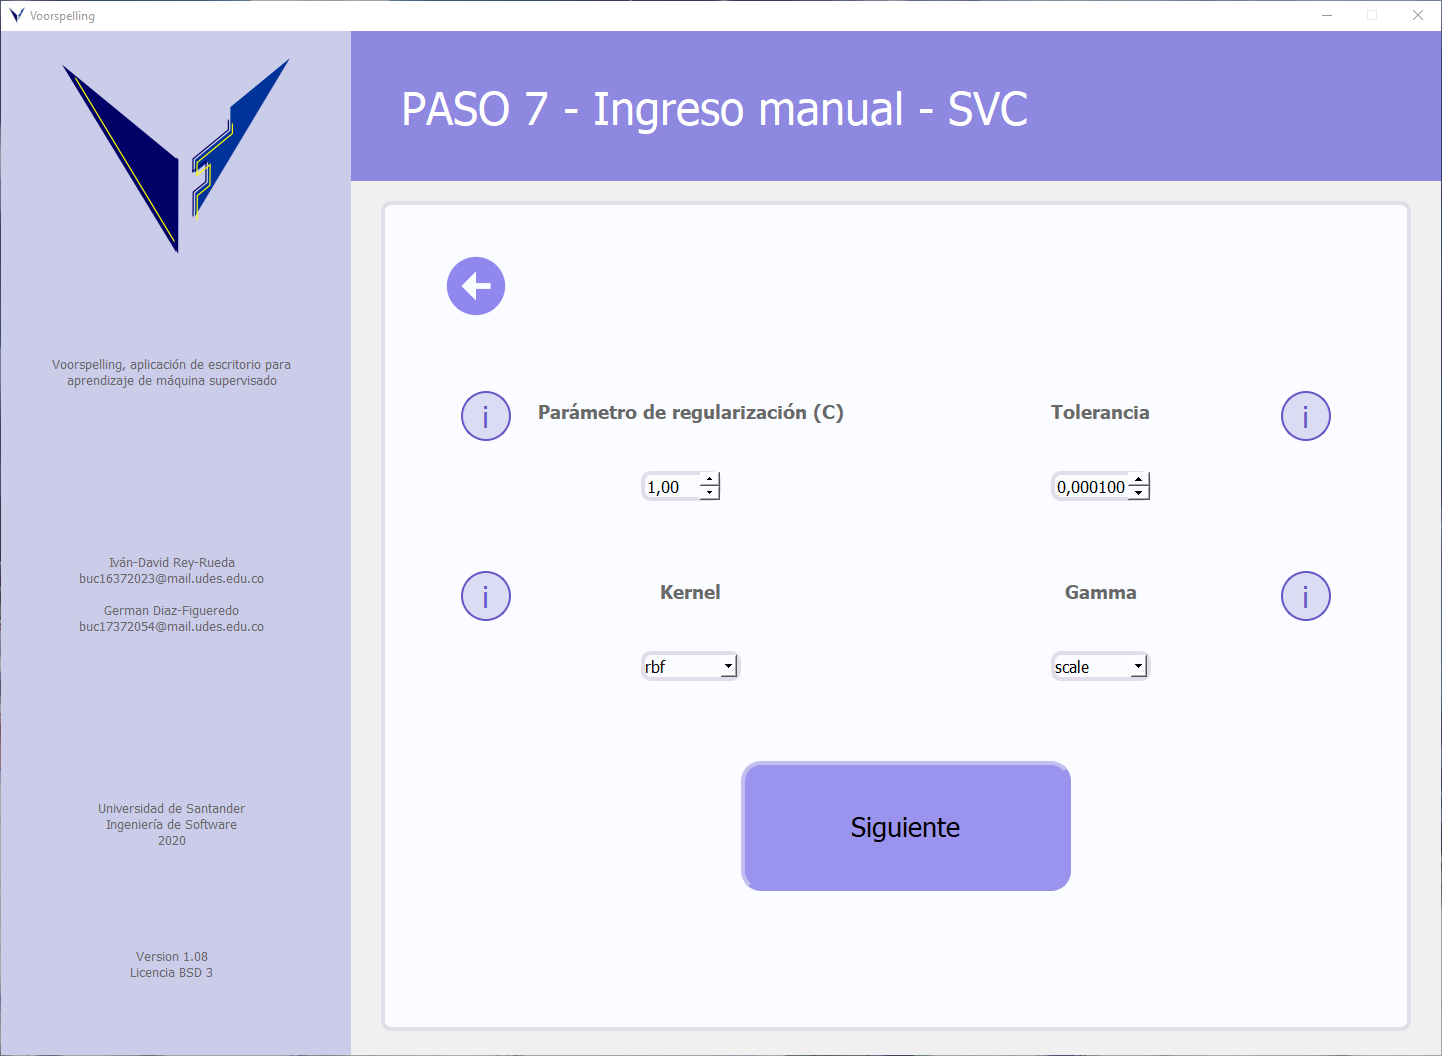
\includegraphics[width=\textwidth]{views/svc.png}
    \label{fig:svc}
\end{figure}

\begin{figure}[H]
    \centering
    \caption{Página: hiperparámetros de Gaussian Naive Bayes}
    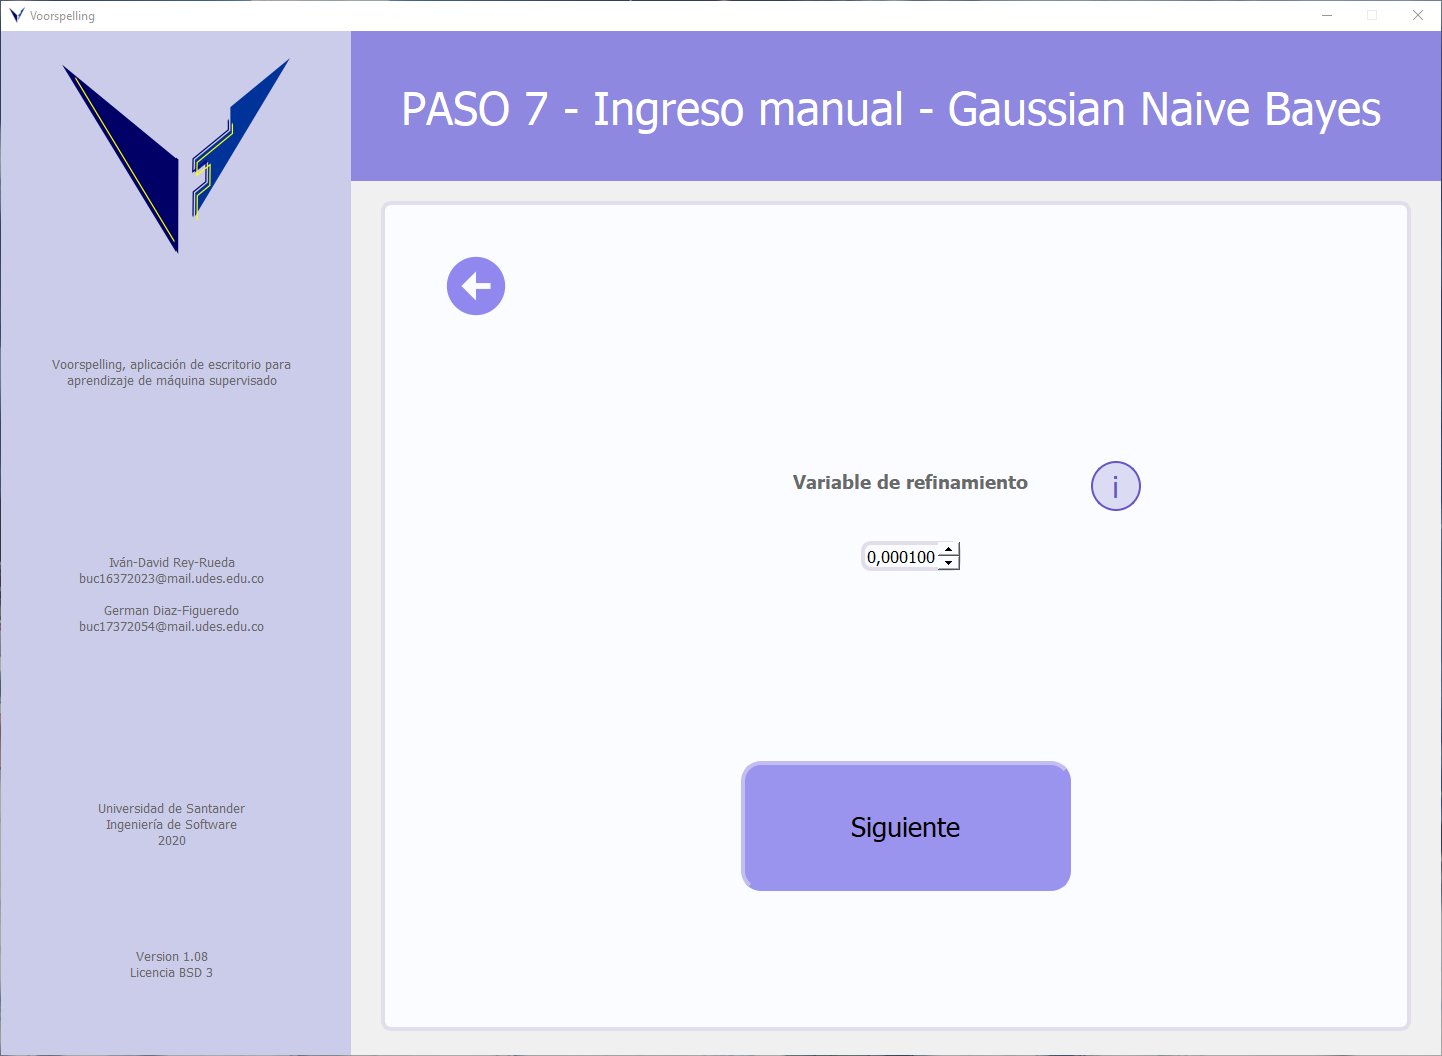
\includegraphics[width=\textwidth]{views/gaussian_naive_bayes.png}
    \label{fig:gassianNB}
\end{figure}

\begin{figure}[H]
    \centering
    \caption{Página: hiperparámetros de Lasso}
    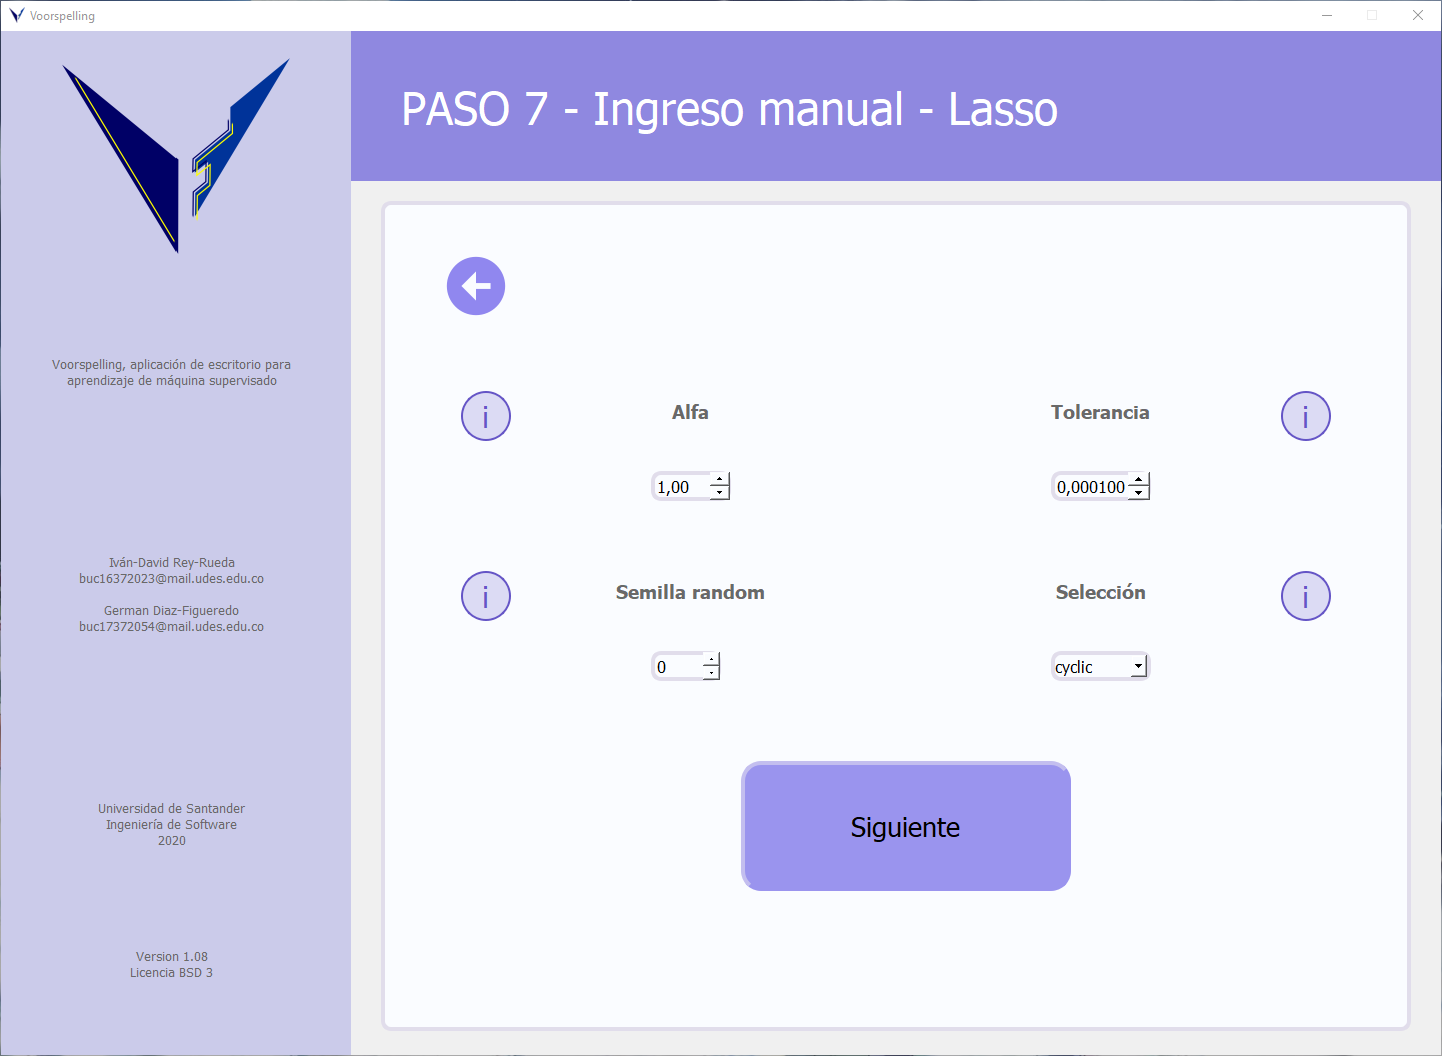
\includegraphics[width=\textwidth]{views/lasso.png}
    \label{fig:lasso}
\end{figure}

\begin{figure}[H]
    \centering
    \caption{Página: hiperparámetros de LinearSVR}
    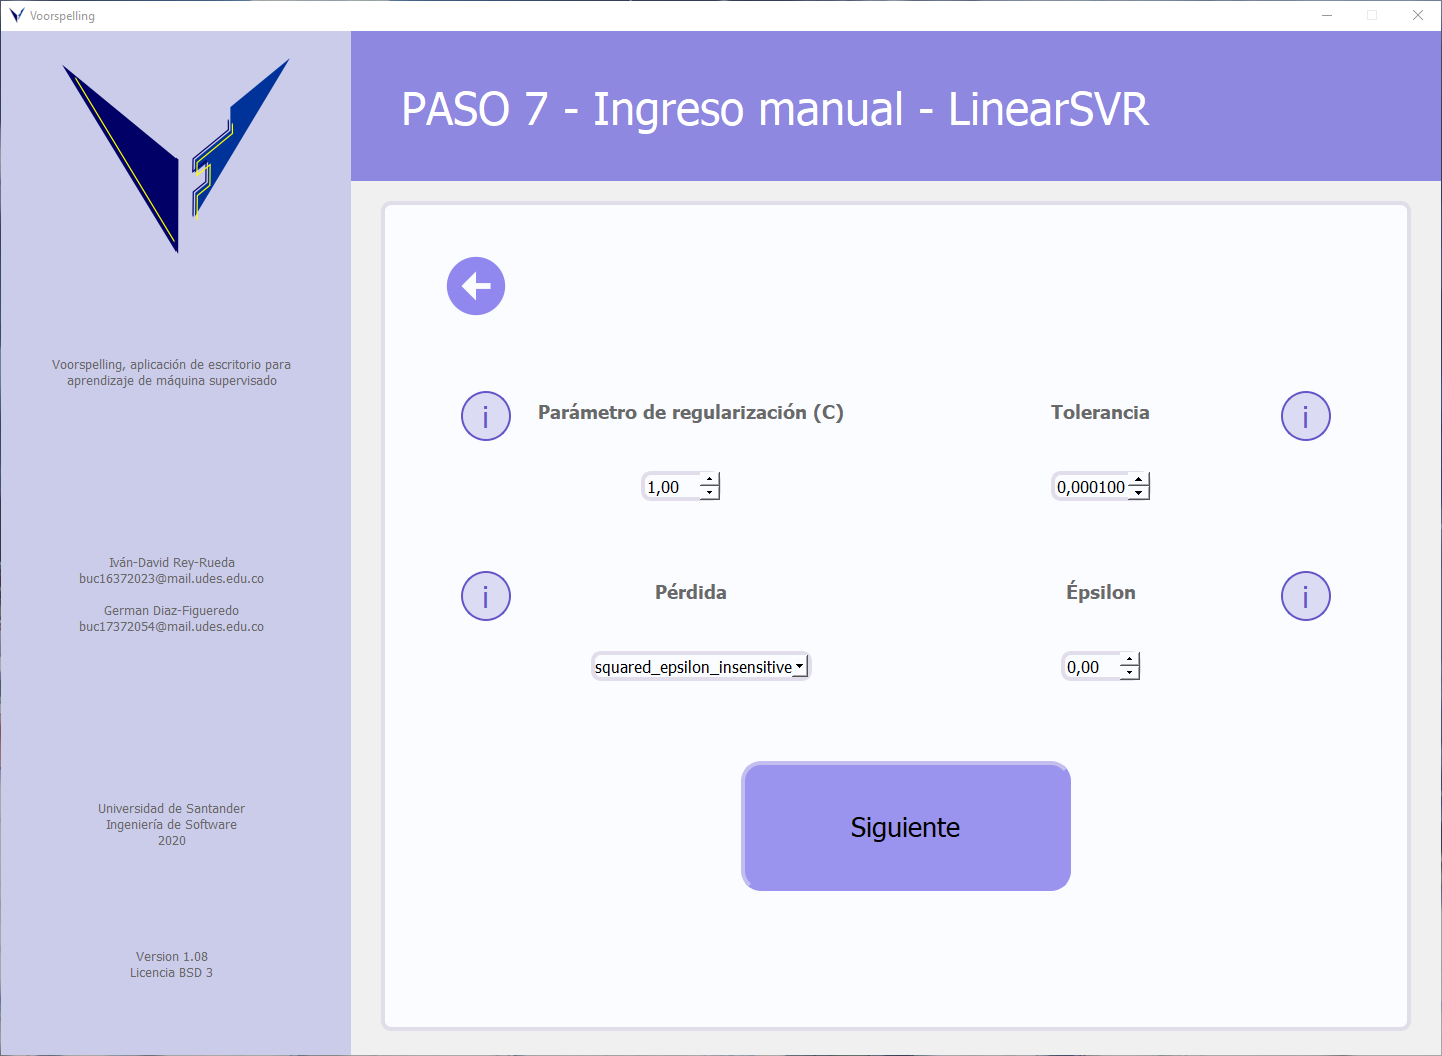
\includegraphics[width=\textwidth]{views/linearsvr.png}
    \label{fig:linearsvr}
\end{figure}

\begin{figure}[H]
    \centering
    \caption{Página: hiperparámetros de SVR}
    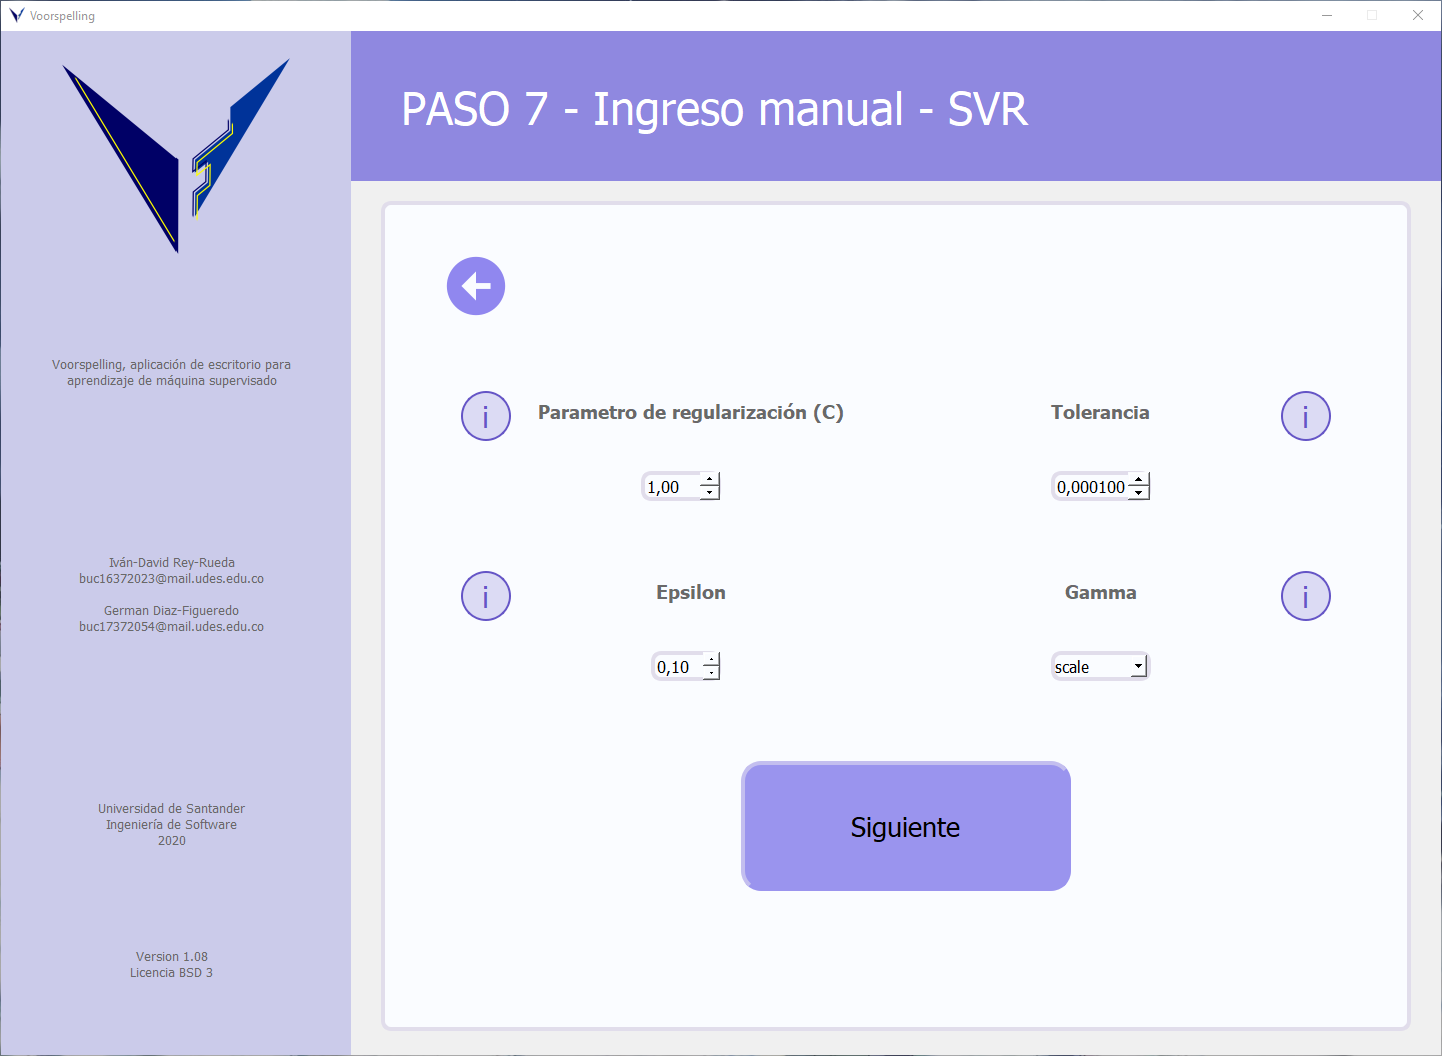
\includegraphics[width=\textwidth]{views/svr.png}
    \label{fig:svr}
\end{figure}

\begin{figure}[H]
    \centering
    \caption{Página: hiperparámetros de SGD}
    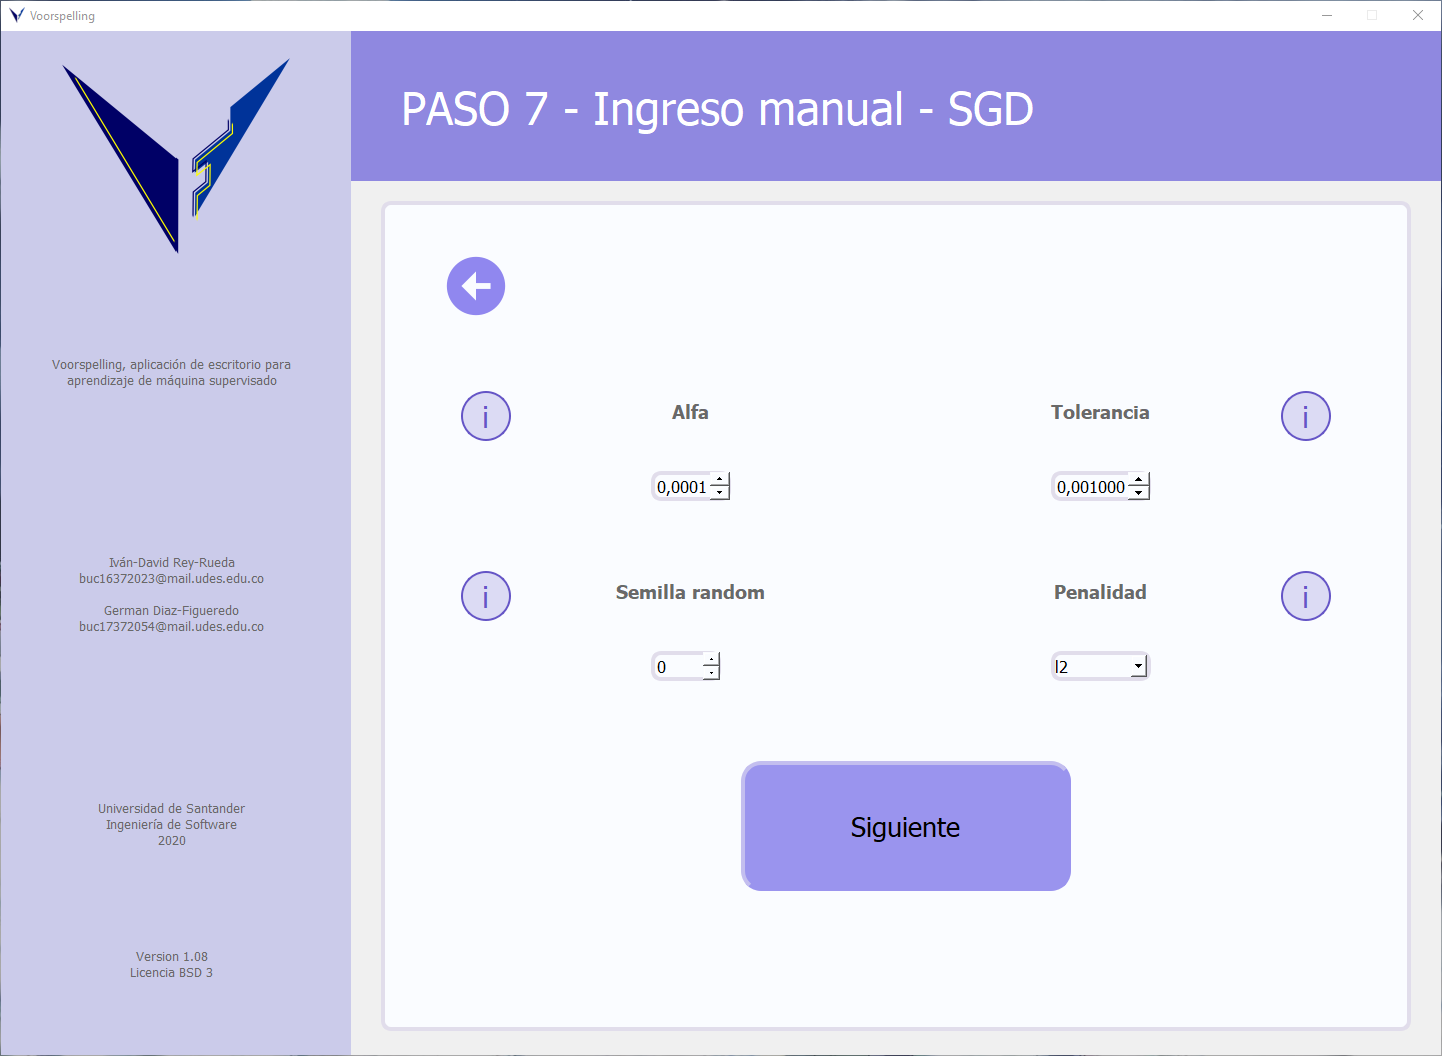
\includegraphics[width=\textwidth]{views/sgd.png}
    \label{fig:sgd}
\end{figure}

\begin{figure}[H]
    \centering
    \caption{Página: hiperparámetros de Affinity Propagation}
    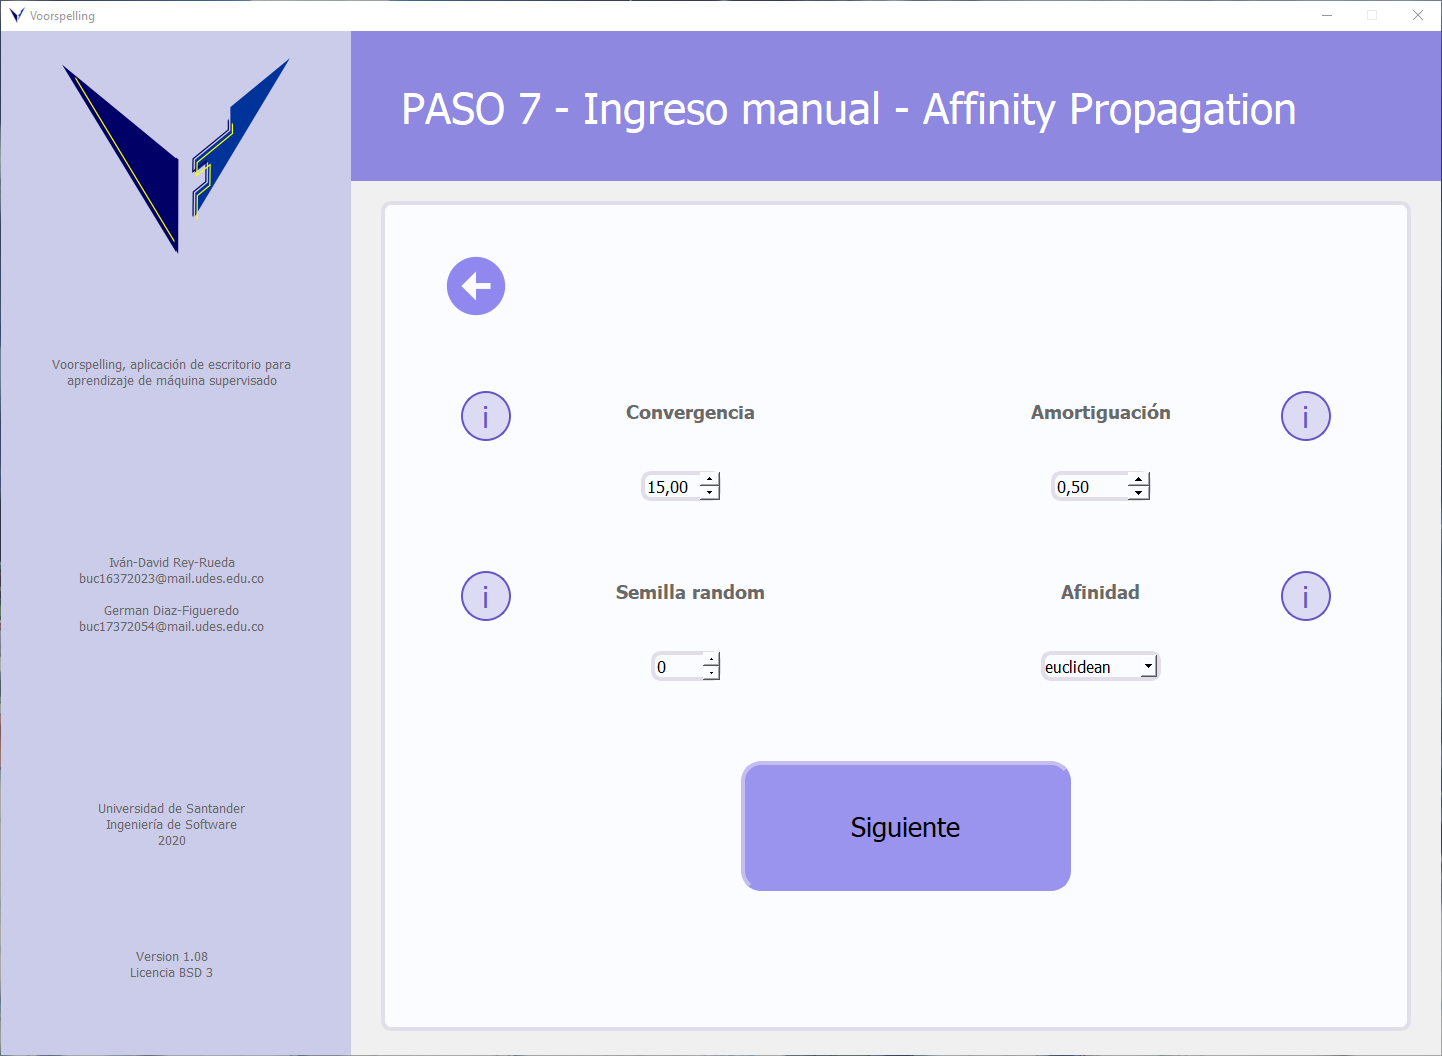
\includegraphics[width=\textwidth]{views/affinity_propagation.png}
    \label{fig:affinitypropagation}
\end{figure}

\begin{figure}[H]
    \centering
    \caption{Página: hiperparámetros de KMeans}
    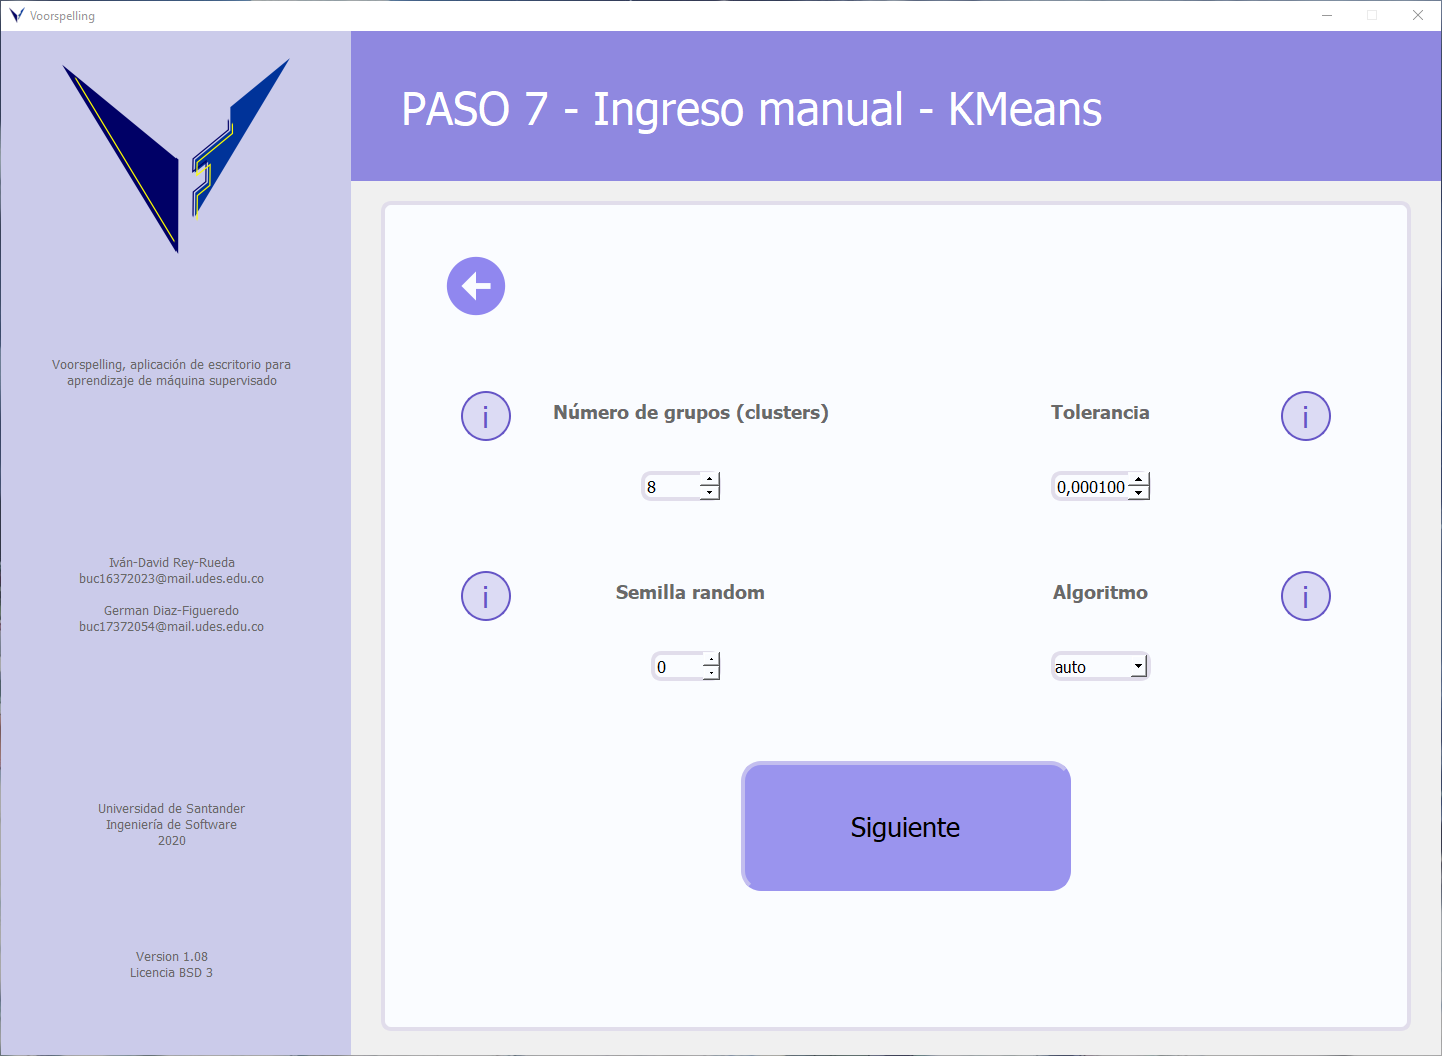
\includegraphics[width=\textwidth]{views/kmeans.png}
    \label{fig:kmeans}
\end{figure}

\begin{figure}[H]
    \centering
    \caption{Página: hiperparámetros de MiniBatch KMeans}
    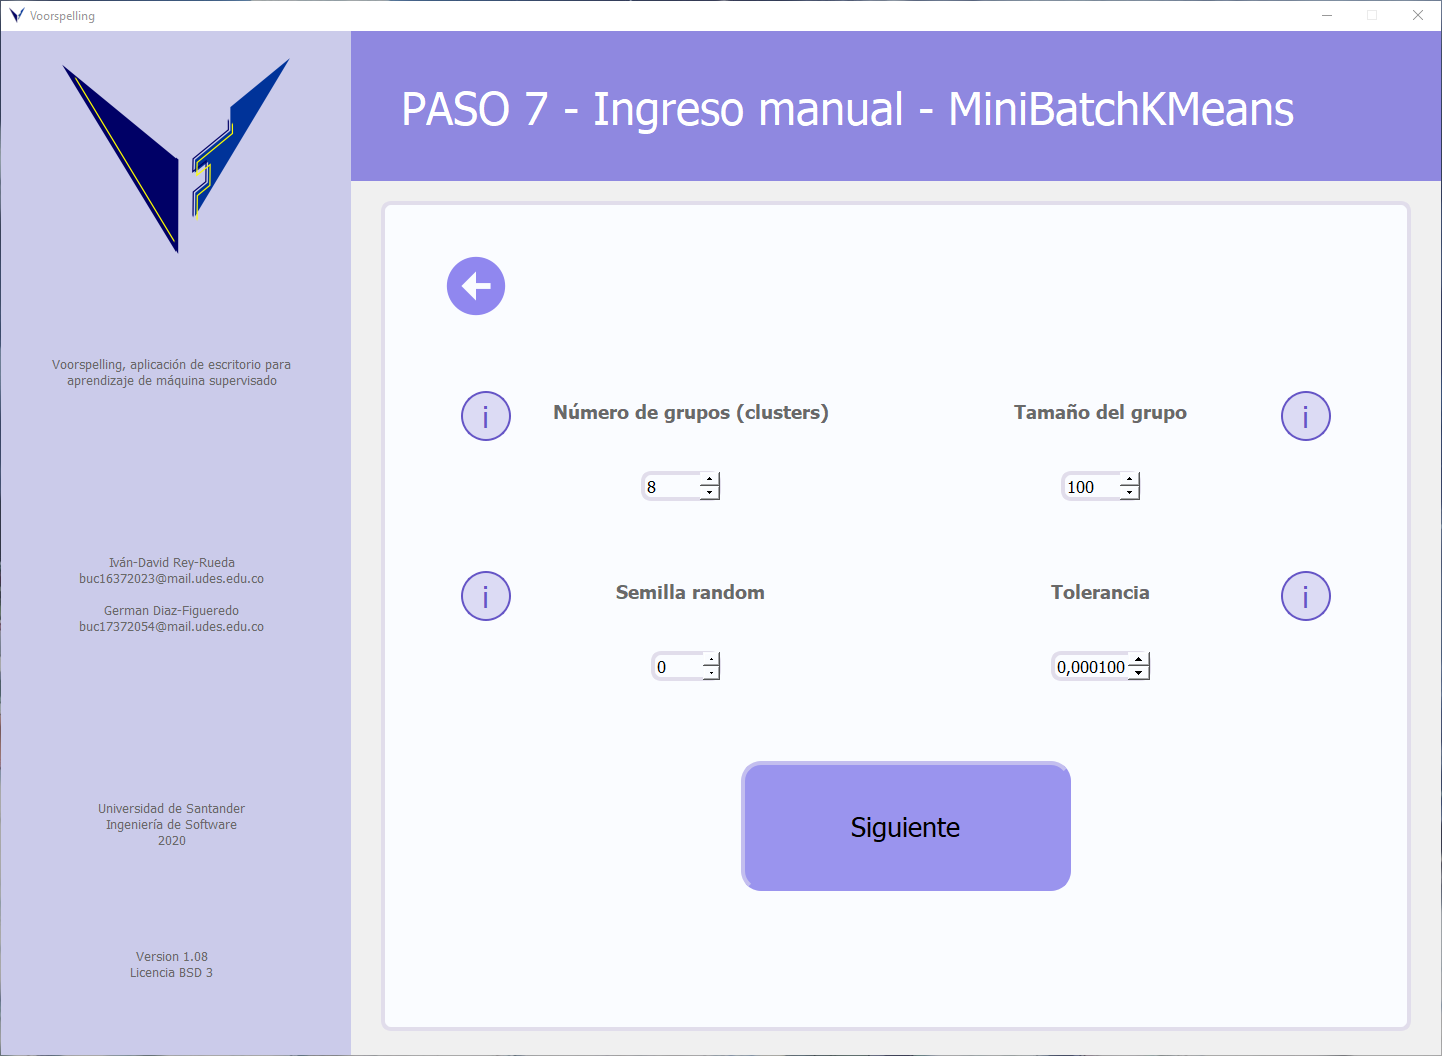
\includegraphics[width=\textwidth]{views/minibatch_kmeans.png}
    \label{fig:minibatchkmeans}
\end{figure}

\begin{figure}[H]
    \centering
    \caption{Página: hiperparámetros de Meanshift}
    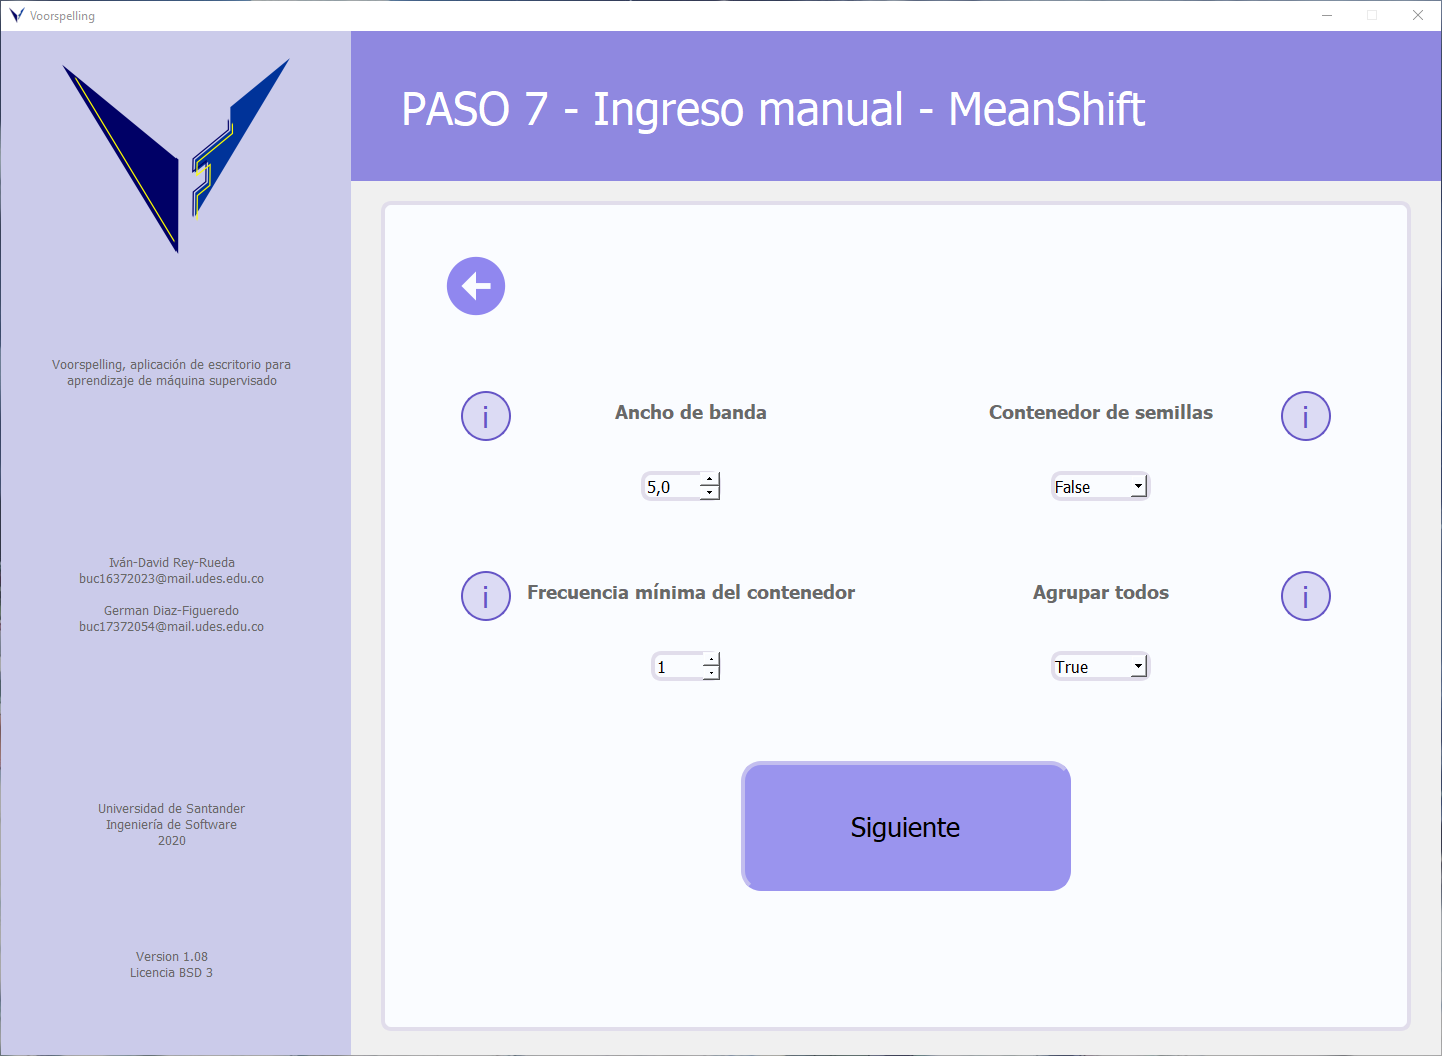
\includegraphics[width=\textwidth]{views/meanshift.png}
    \label{fig:meanshift}
\end{figure}

\section{Documentación}
Los archivos relacionados a la documentación del proyecto Voorspelling se encuentran en la carpeta \textit{Documentation} del repositorio del proyecto, la cual puede ser consultada en GitHub con el siguiente enlace: \url{https://github.com/Noczio/VoorSpelling}.

Cada carpeta contiene archivos clasificados por su tipo, ya sean diagramas, formatos, flujo de la aplicación, \textit{mockups}, \textit{sketchs} y otros recursos como el cronograma del proyecto. No obstante, los documentos que se presentan a continuación son aquellos relacionados con los requerimientos, \textit{back-end}, \textit{front-end} y casos de uso  desarrollados durante el ciclo de vida del proyecto desde Agosto del 2020 hasta Marzo del 2021.

%requerimientos
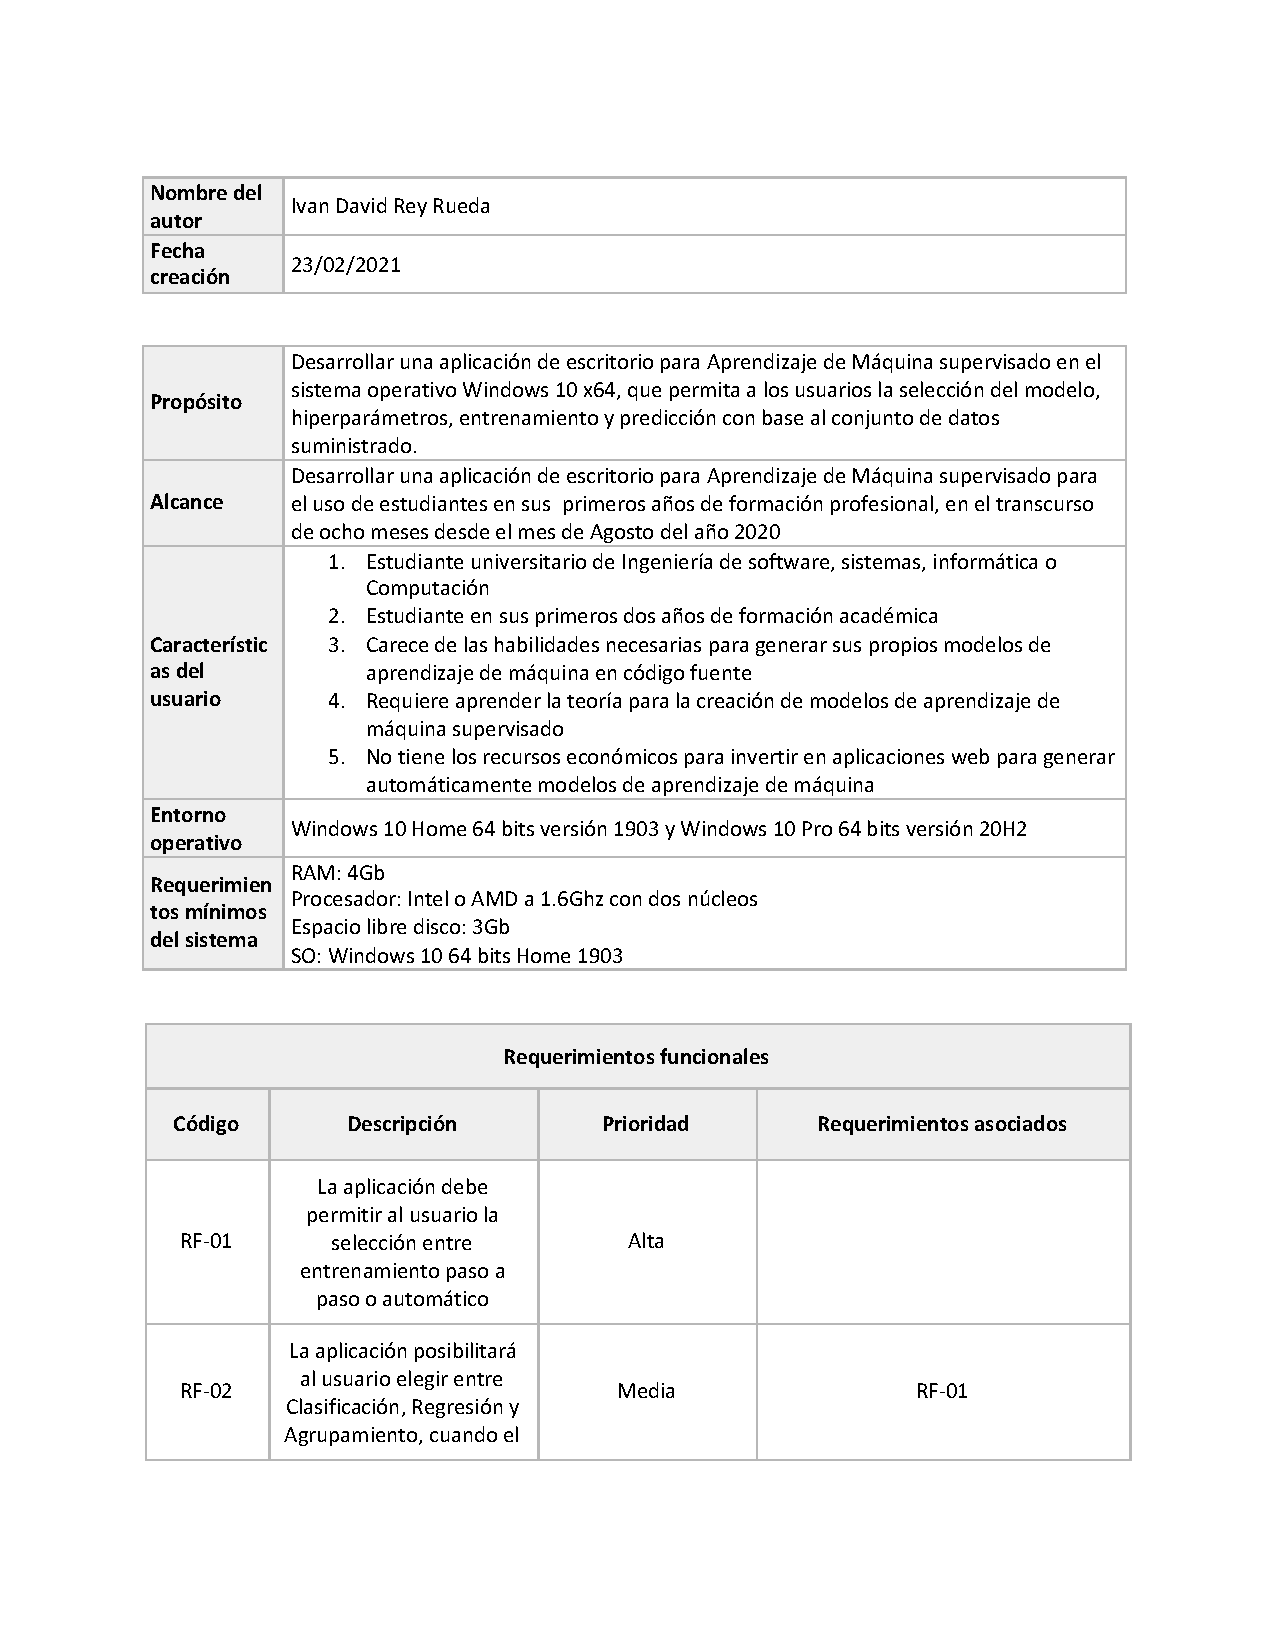
\includepdf[pages=-, pagecommand=\thispagestyle{otherplain} ,width=\textwidth]{pdfs/Requerimientos_proyecto_Firmado.pdf}
%front y back end
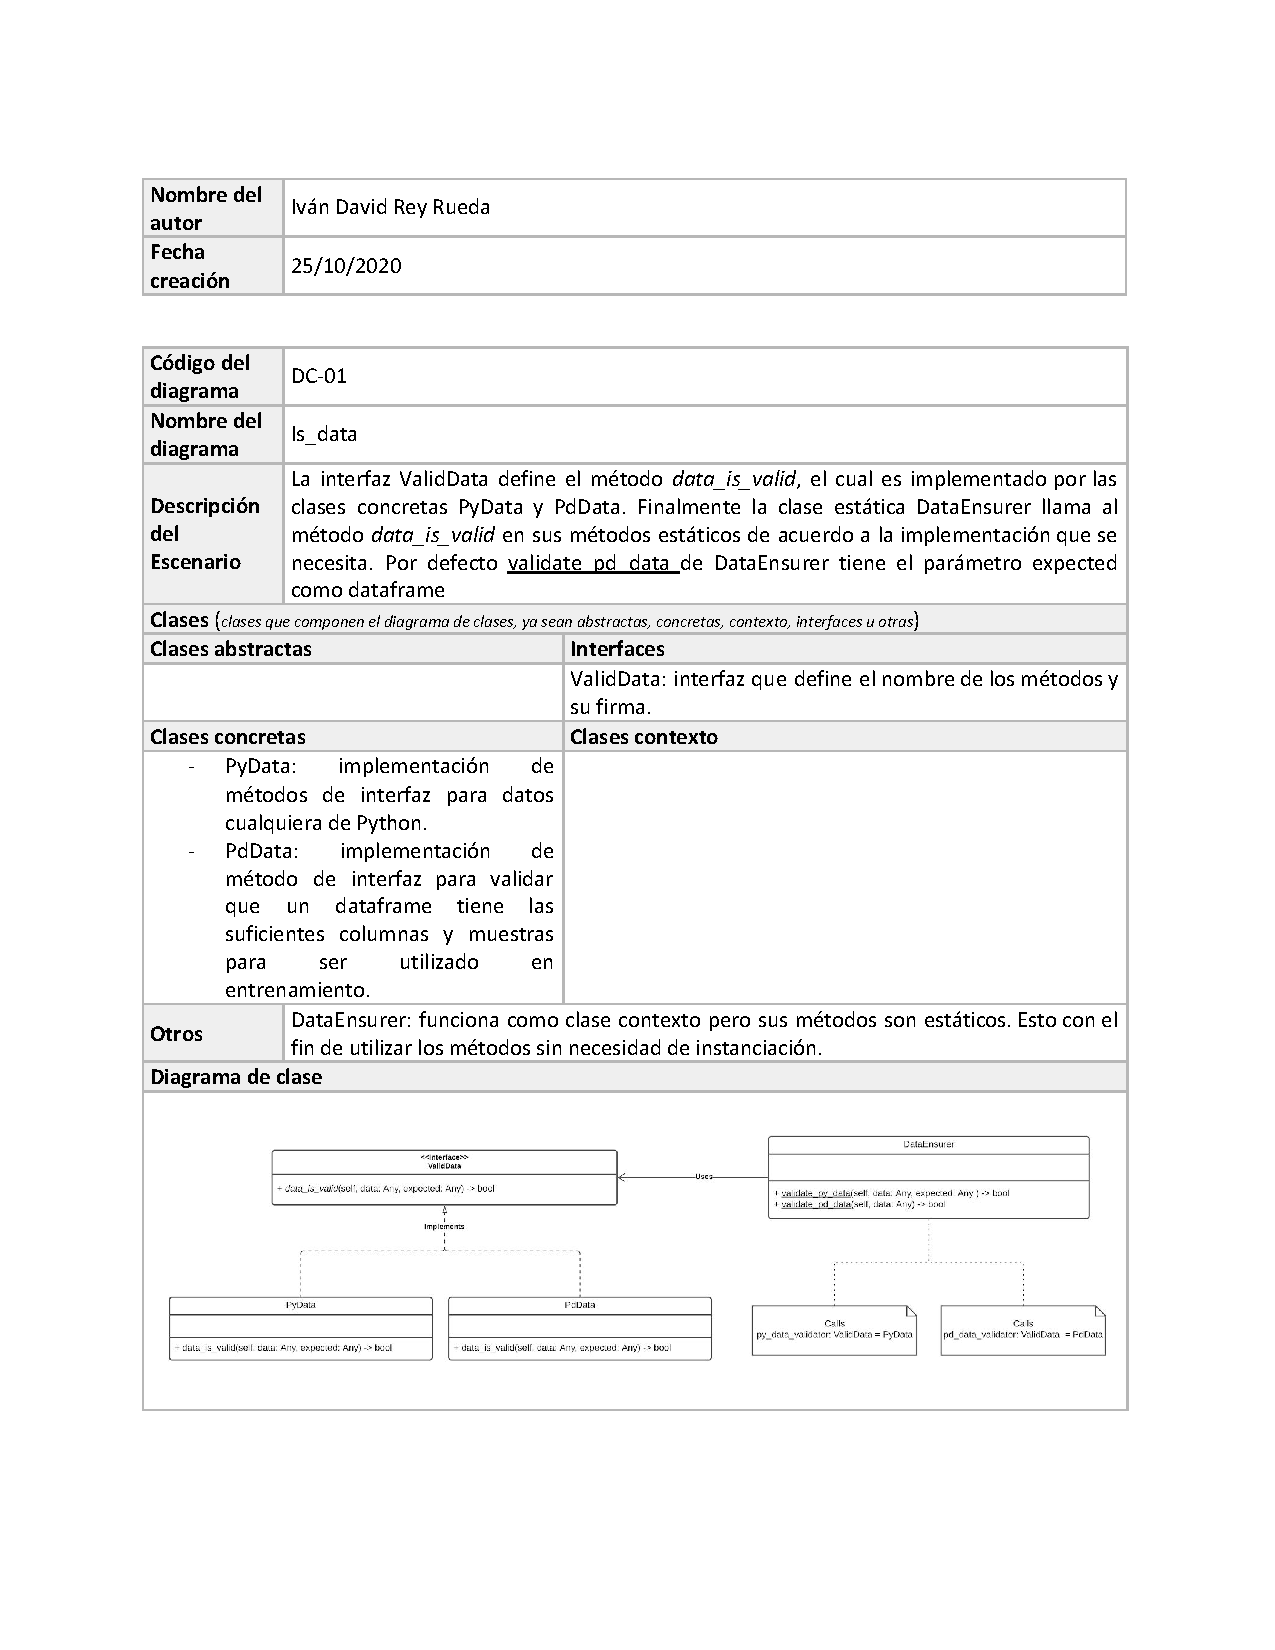
\includepdf[pages=-, pagecommand=\thispagestyle{otherplain} ,width=\textwidth]{pdfs/Formato diagrama de clase DC-01_Firmado.pdf}
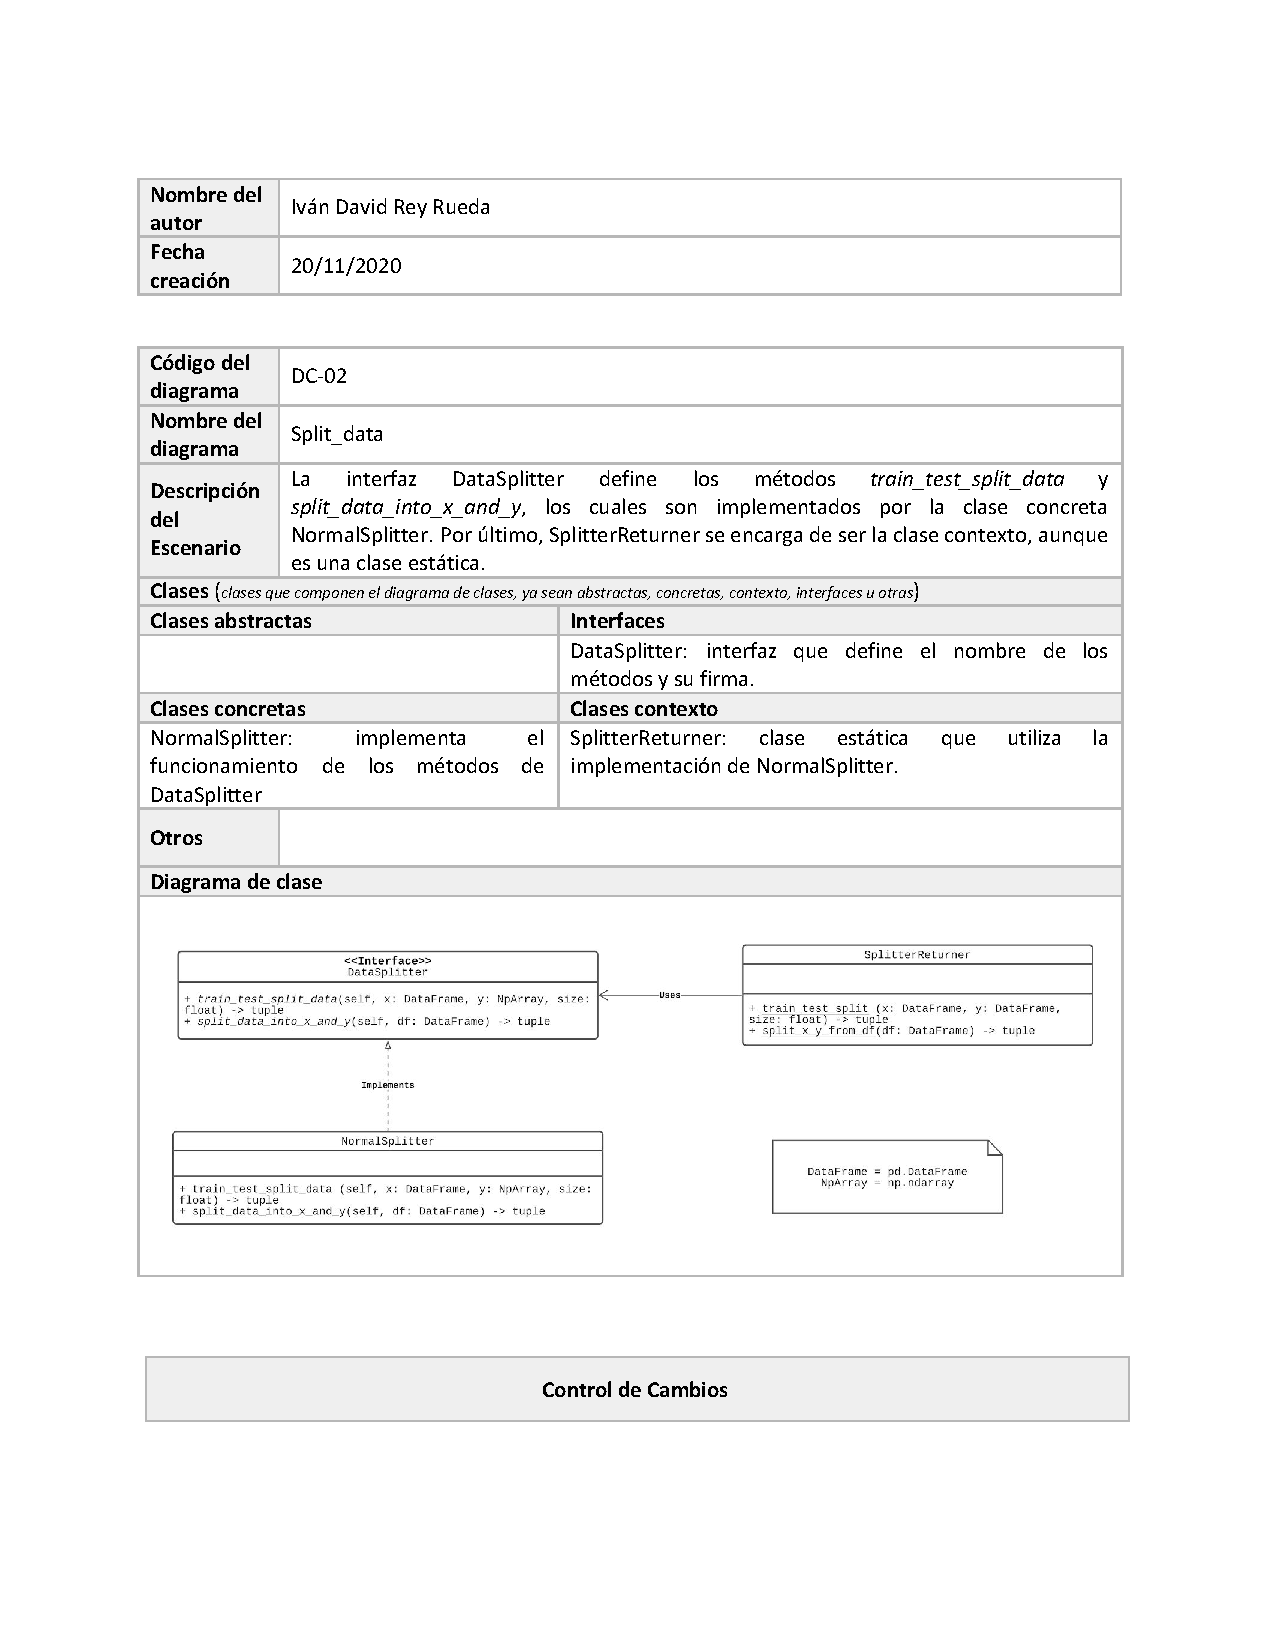
\includepdf[pages=-, pagecommand=\thispagestyle{otherplain}, width=\textwidth]{pdfs/Formato diagrama de clase DC-02_Firmado.pdf}
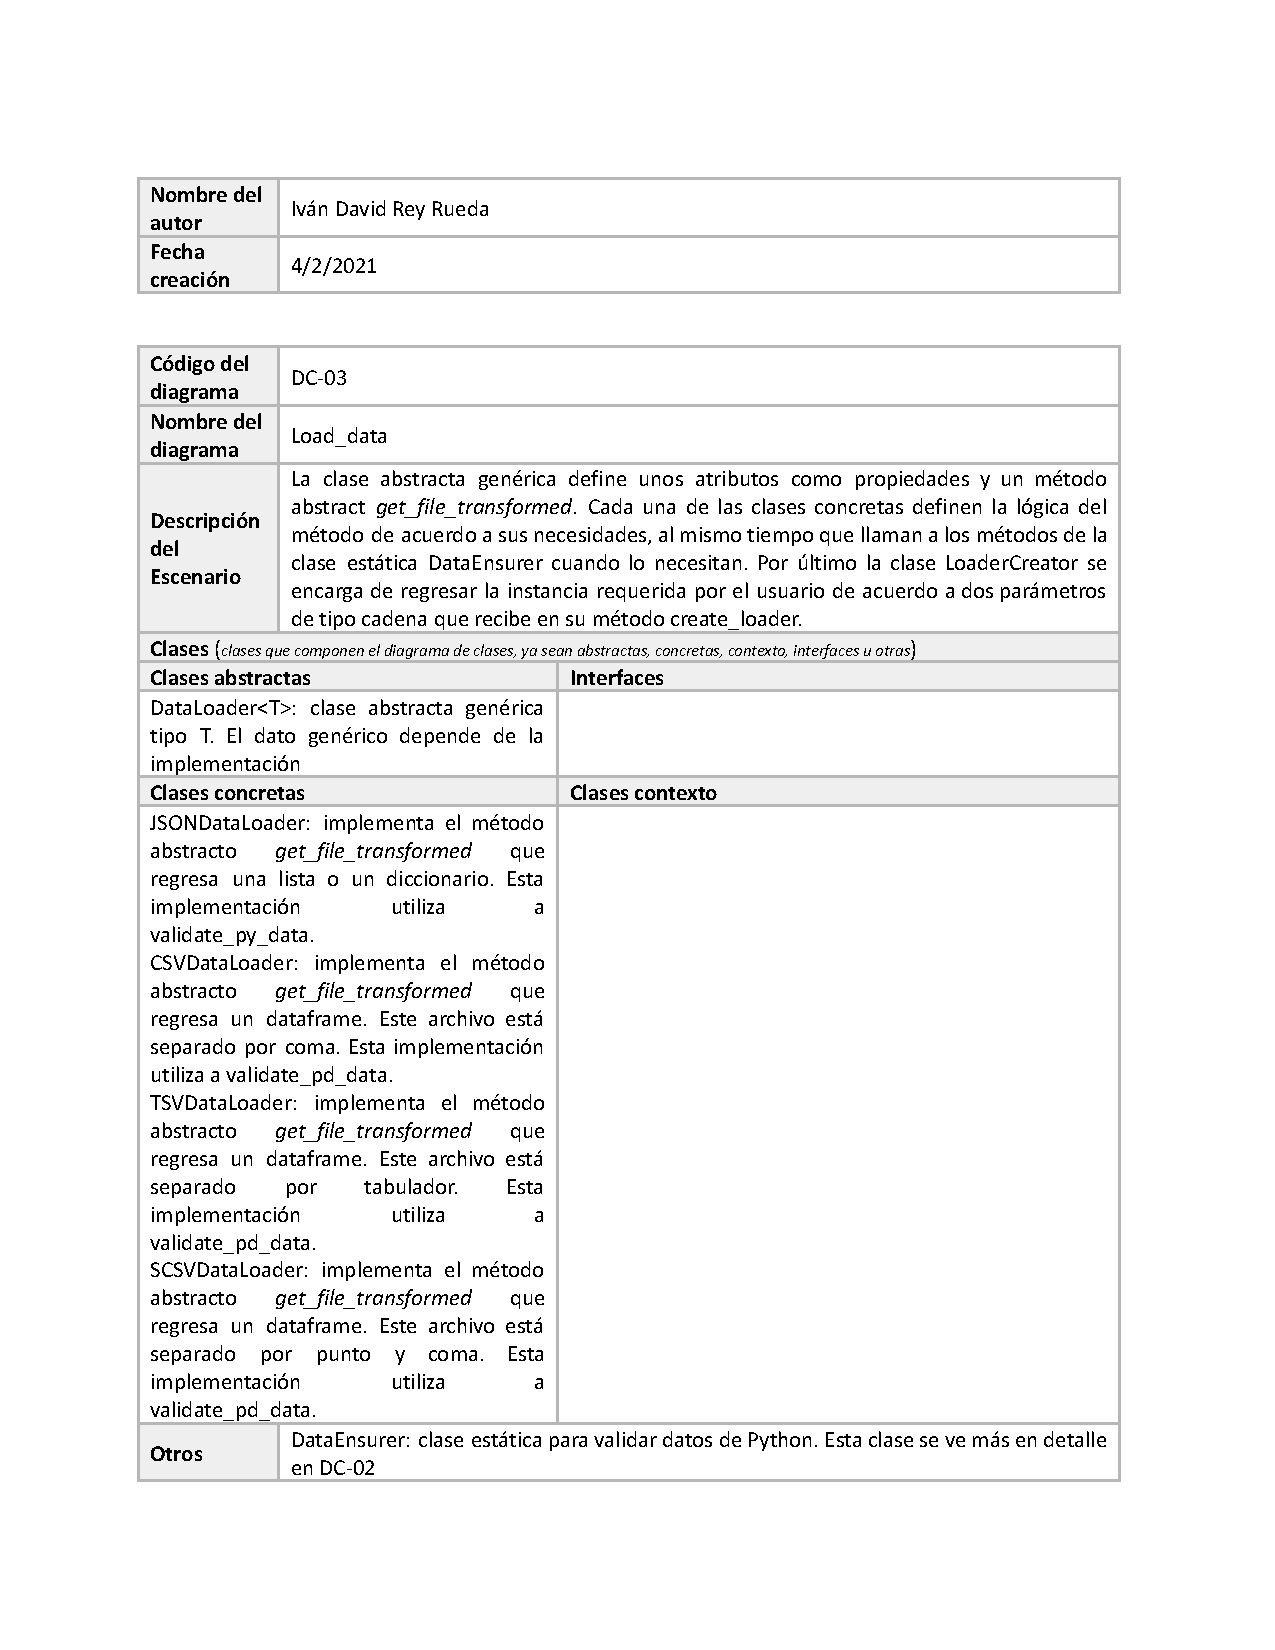
\includepdf[pages=-, pagecommand=\thispagestyle{otherplain}, width=\textwidth]{pdfs/Formato diagrama de clase DC-03_Firmado.pdf}
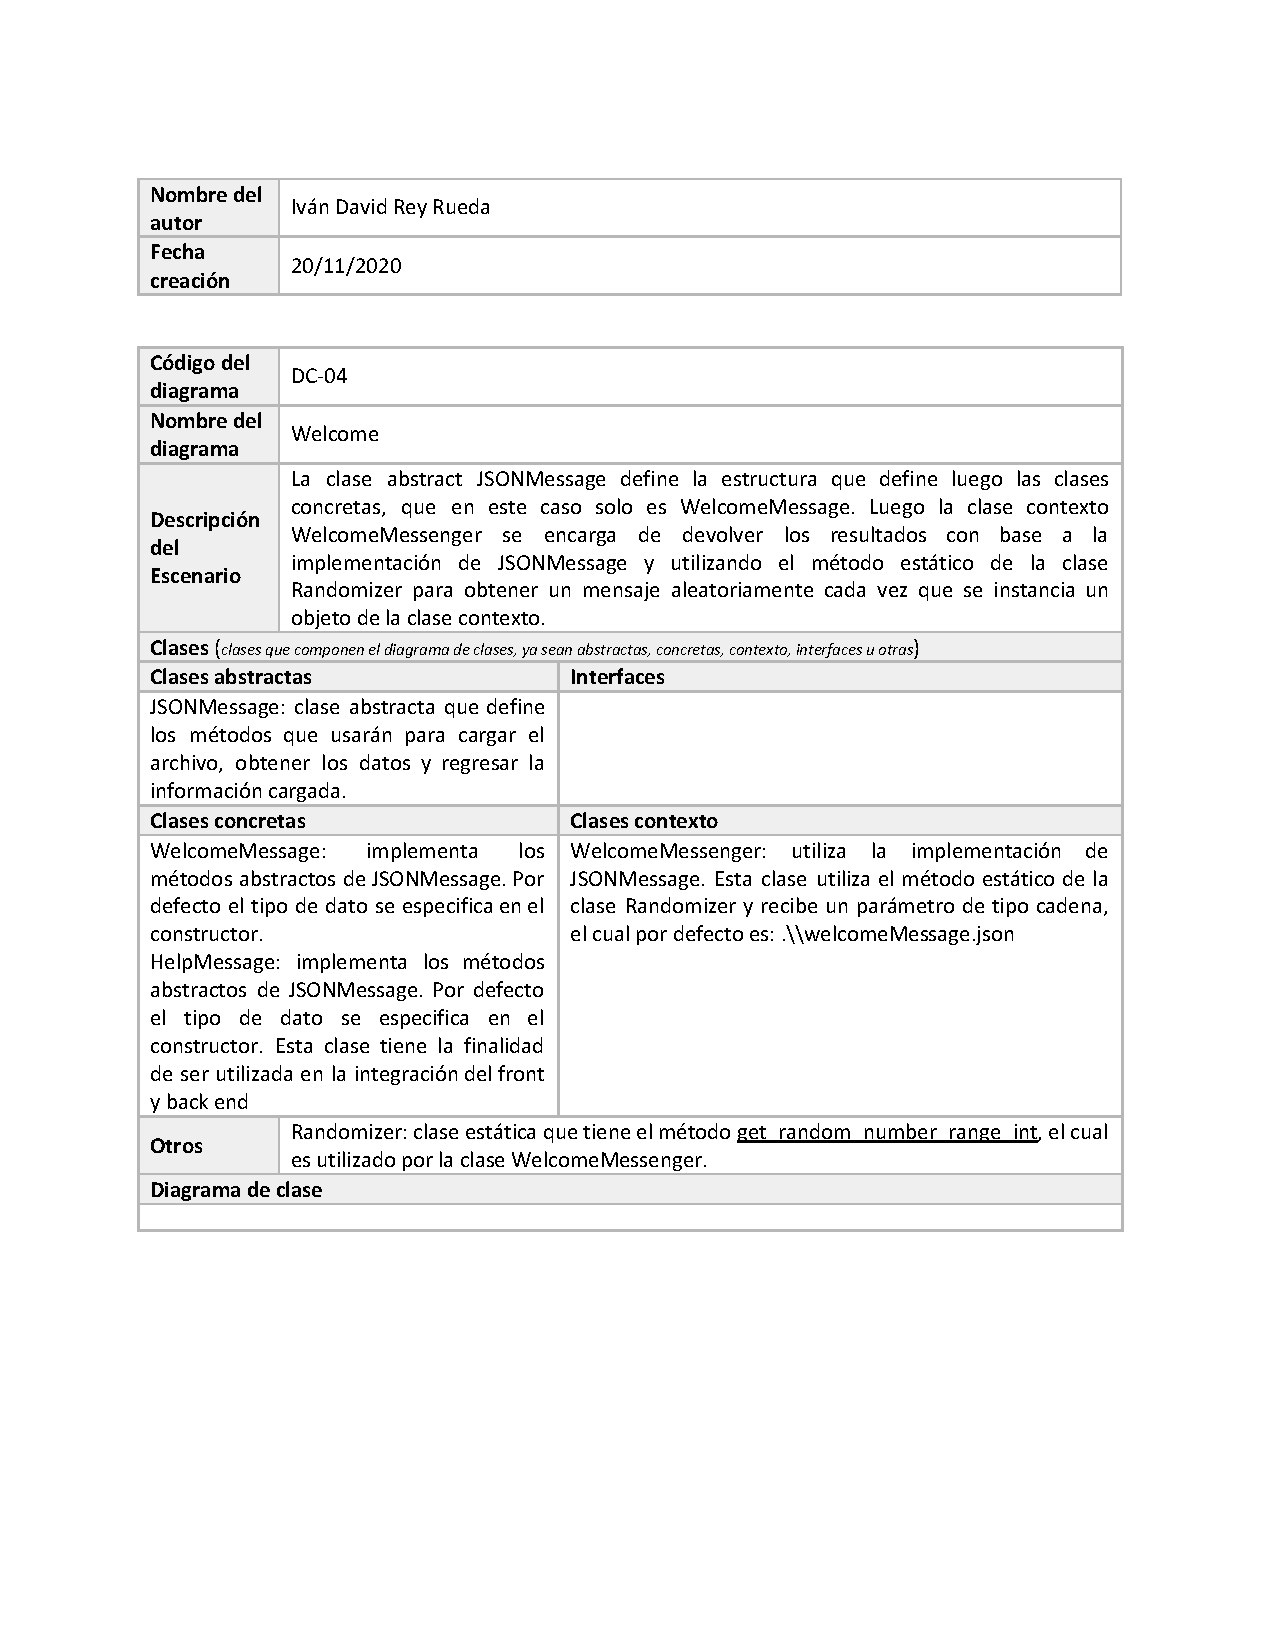
\includepdf[pages=-, pagecommand=\thispagestyle{otherplain}, width=\textwidth]{pdfs/Formato diagrama de clase DC-04_Firmado.pdf}
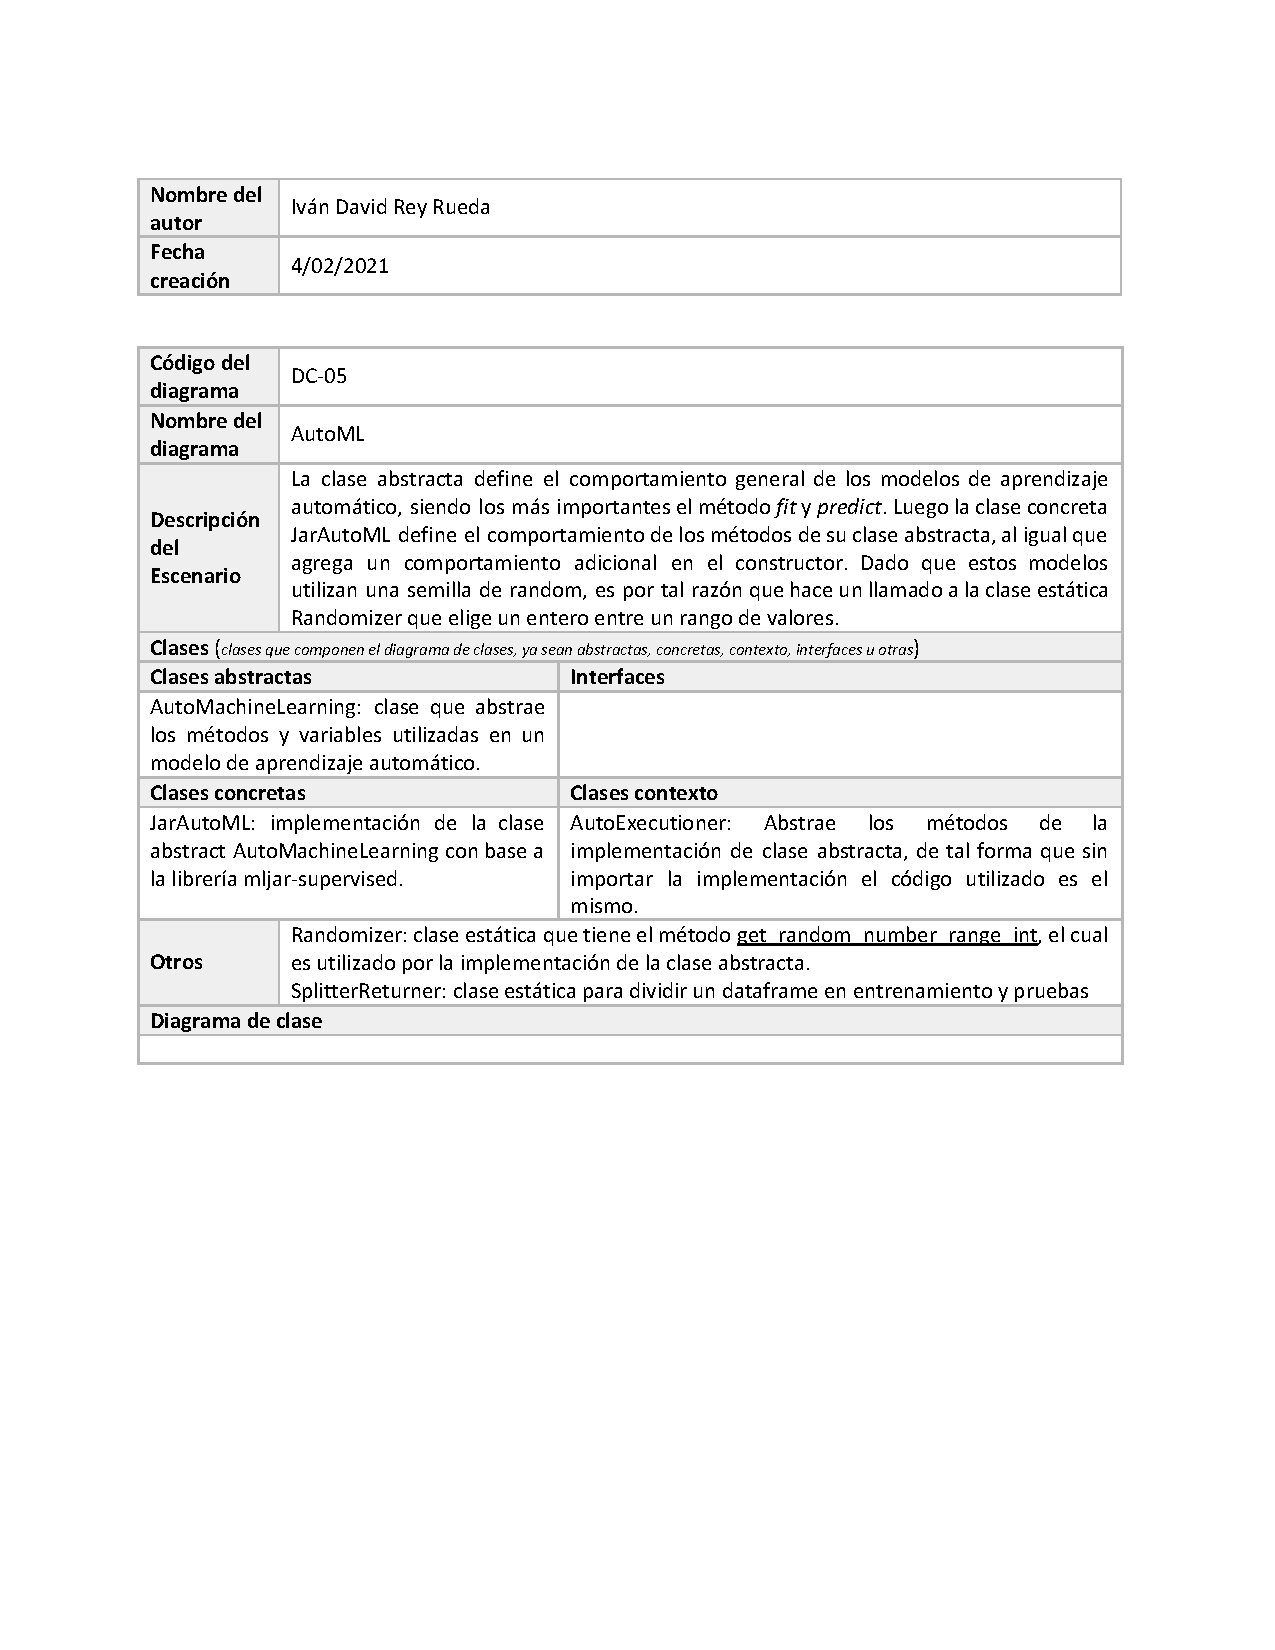
\includepdf[pages=-,pagecommand=\thispagestyle{otherplain}, width=\textwidth]{pdfs/Formato diagrama de clase DC-05_Firmado.pdf}
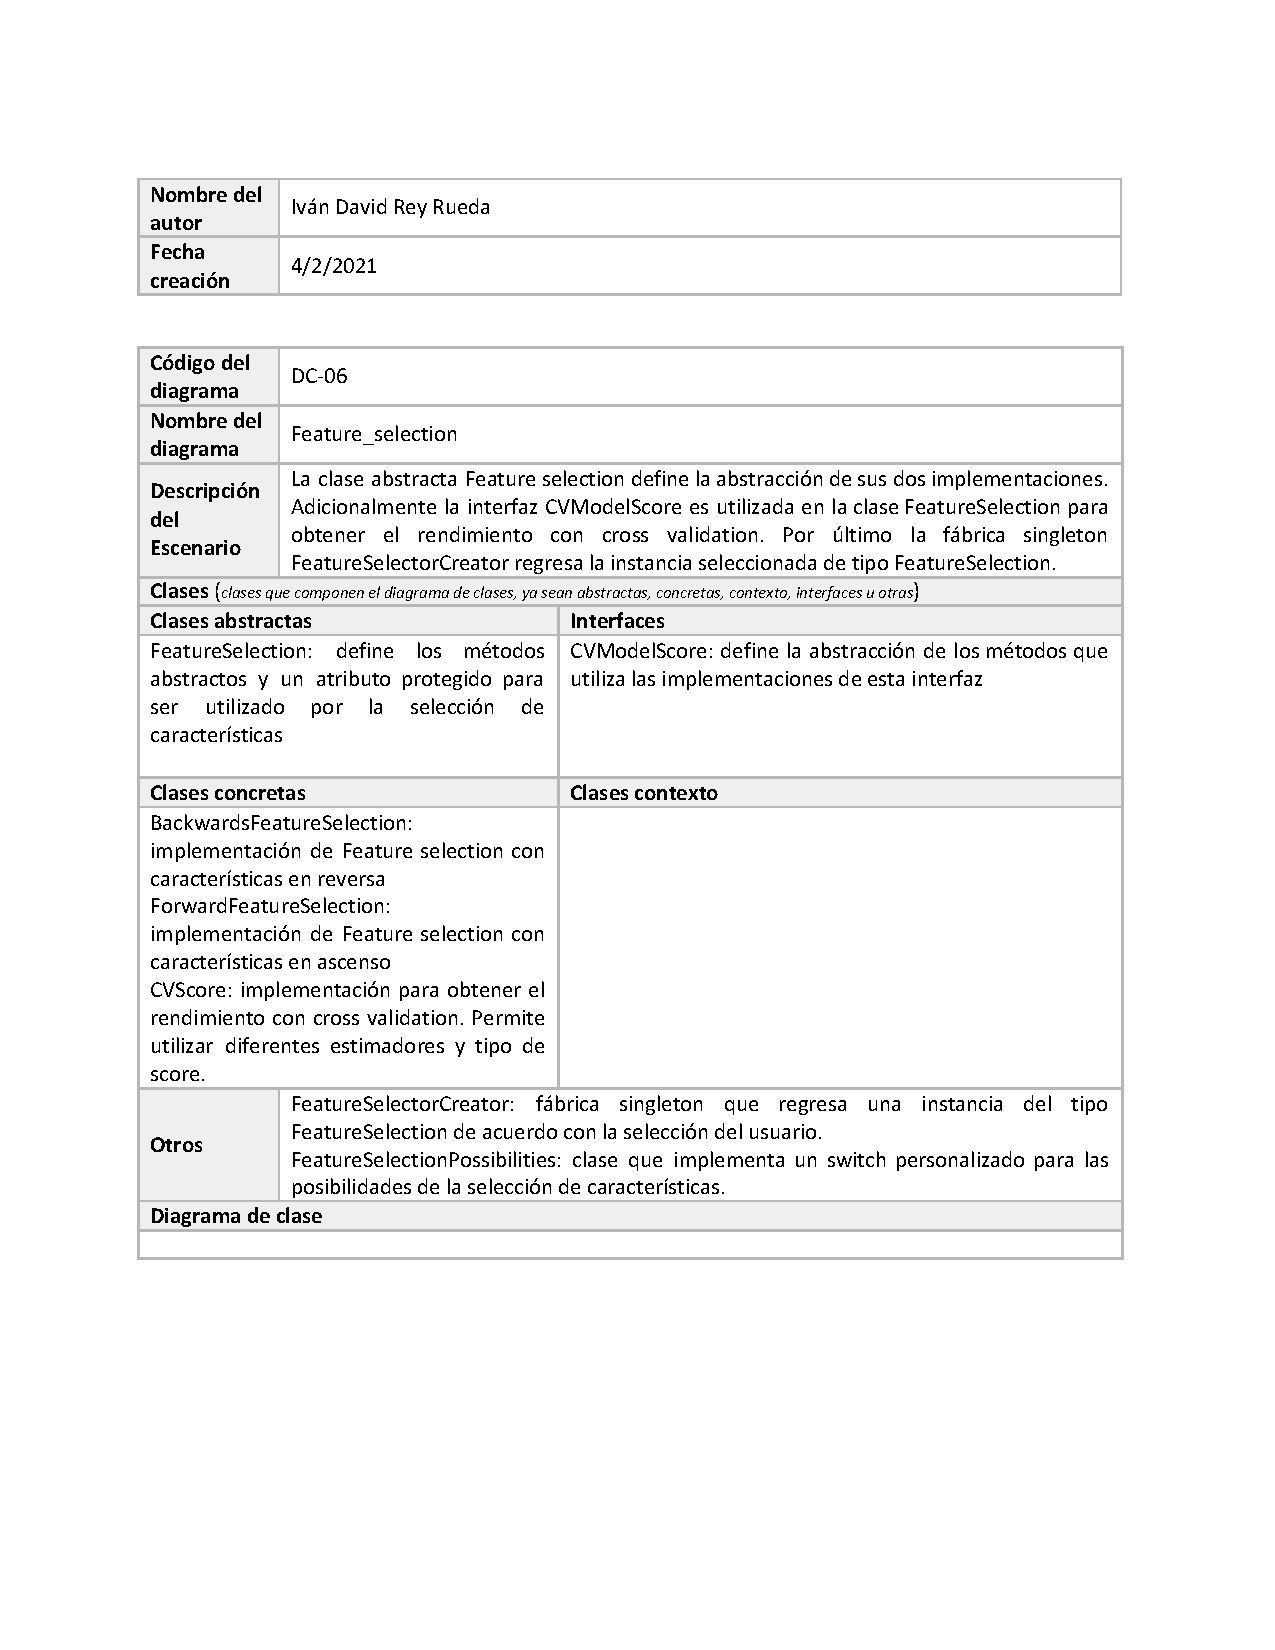
\includepdf[pages=-, pagecommand=\thispagestyle{otherplain}, width=\textwidth]{pdfs/Formato diagrama de clase DC-06_Firmado.pdf}
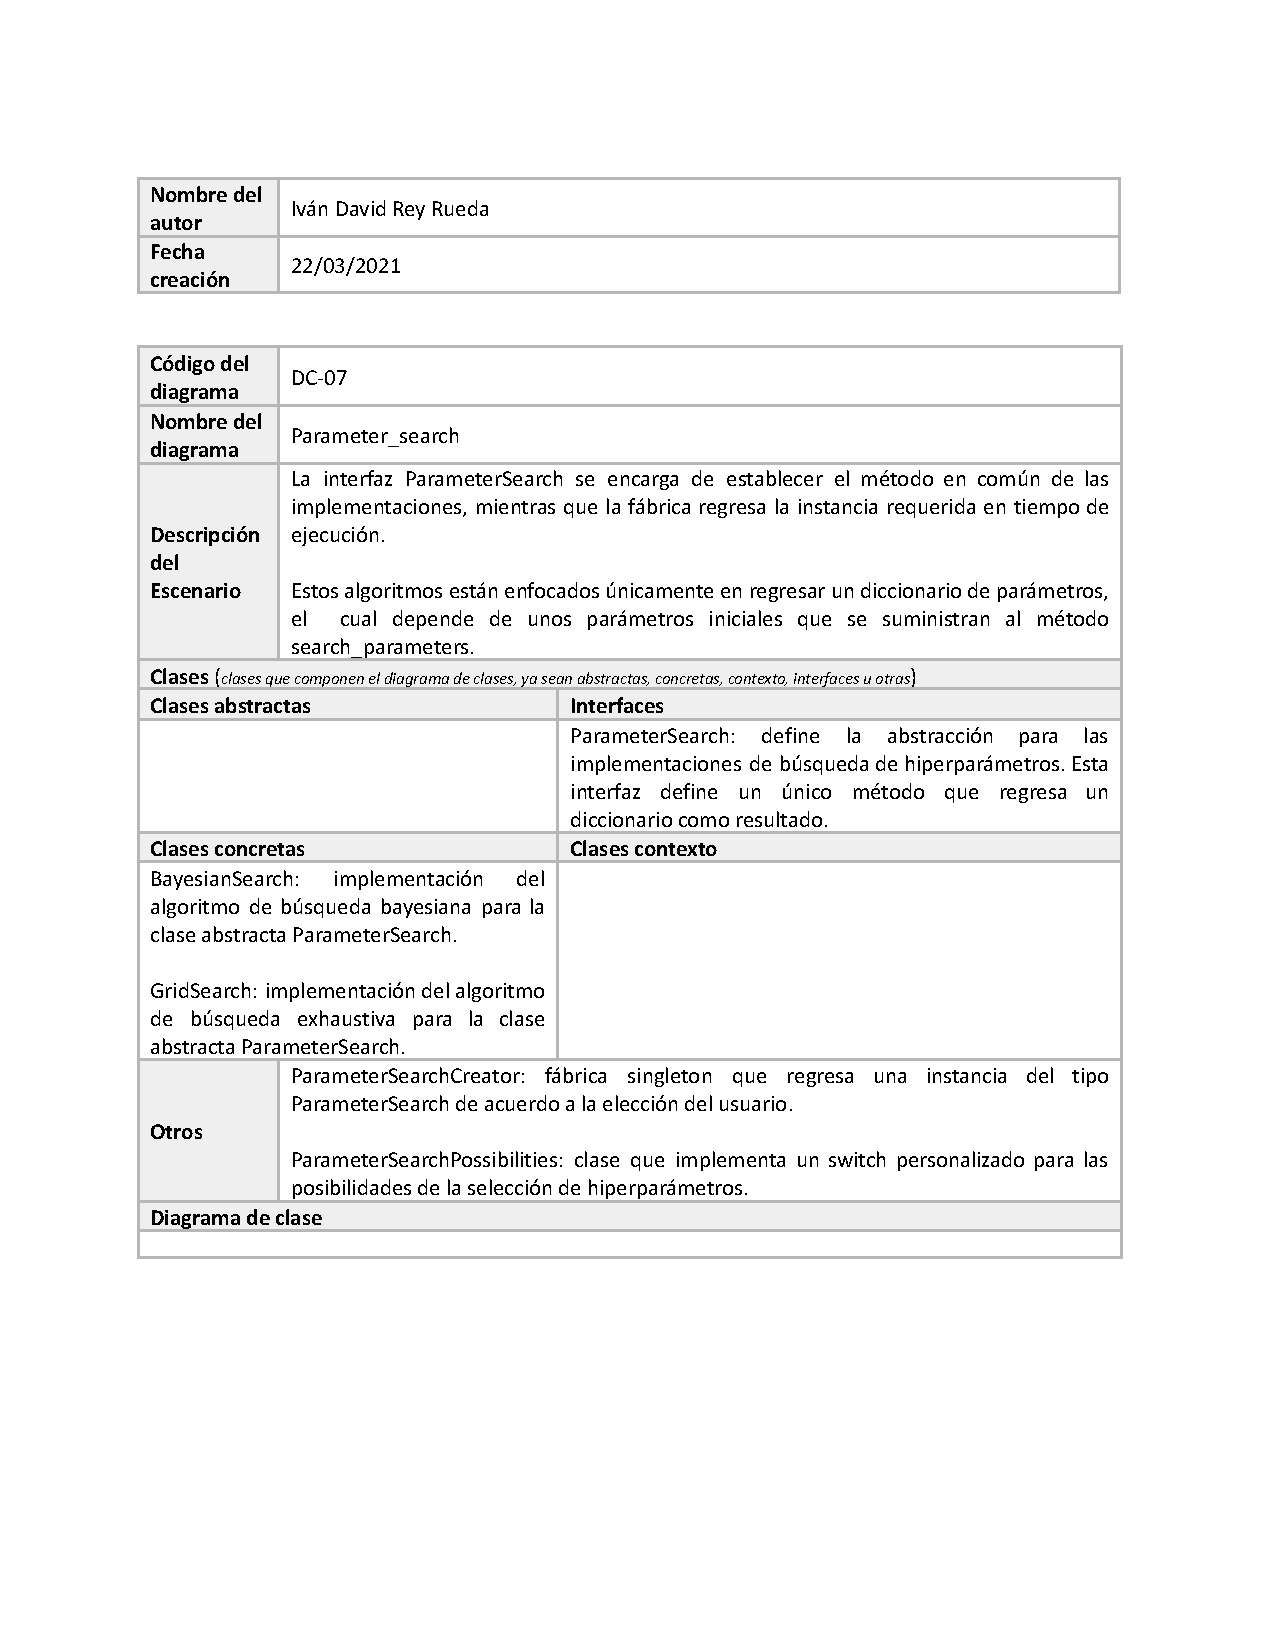
\includepdf[pages=-, pagecommand=\thispagestyle{otherplain}, width=\textwidth]{pdfs/Formato diagrama de clase DC-07_Firmado.pdf}
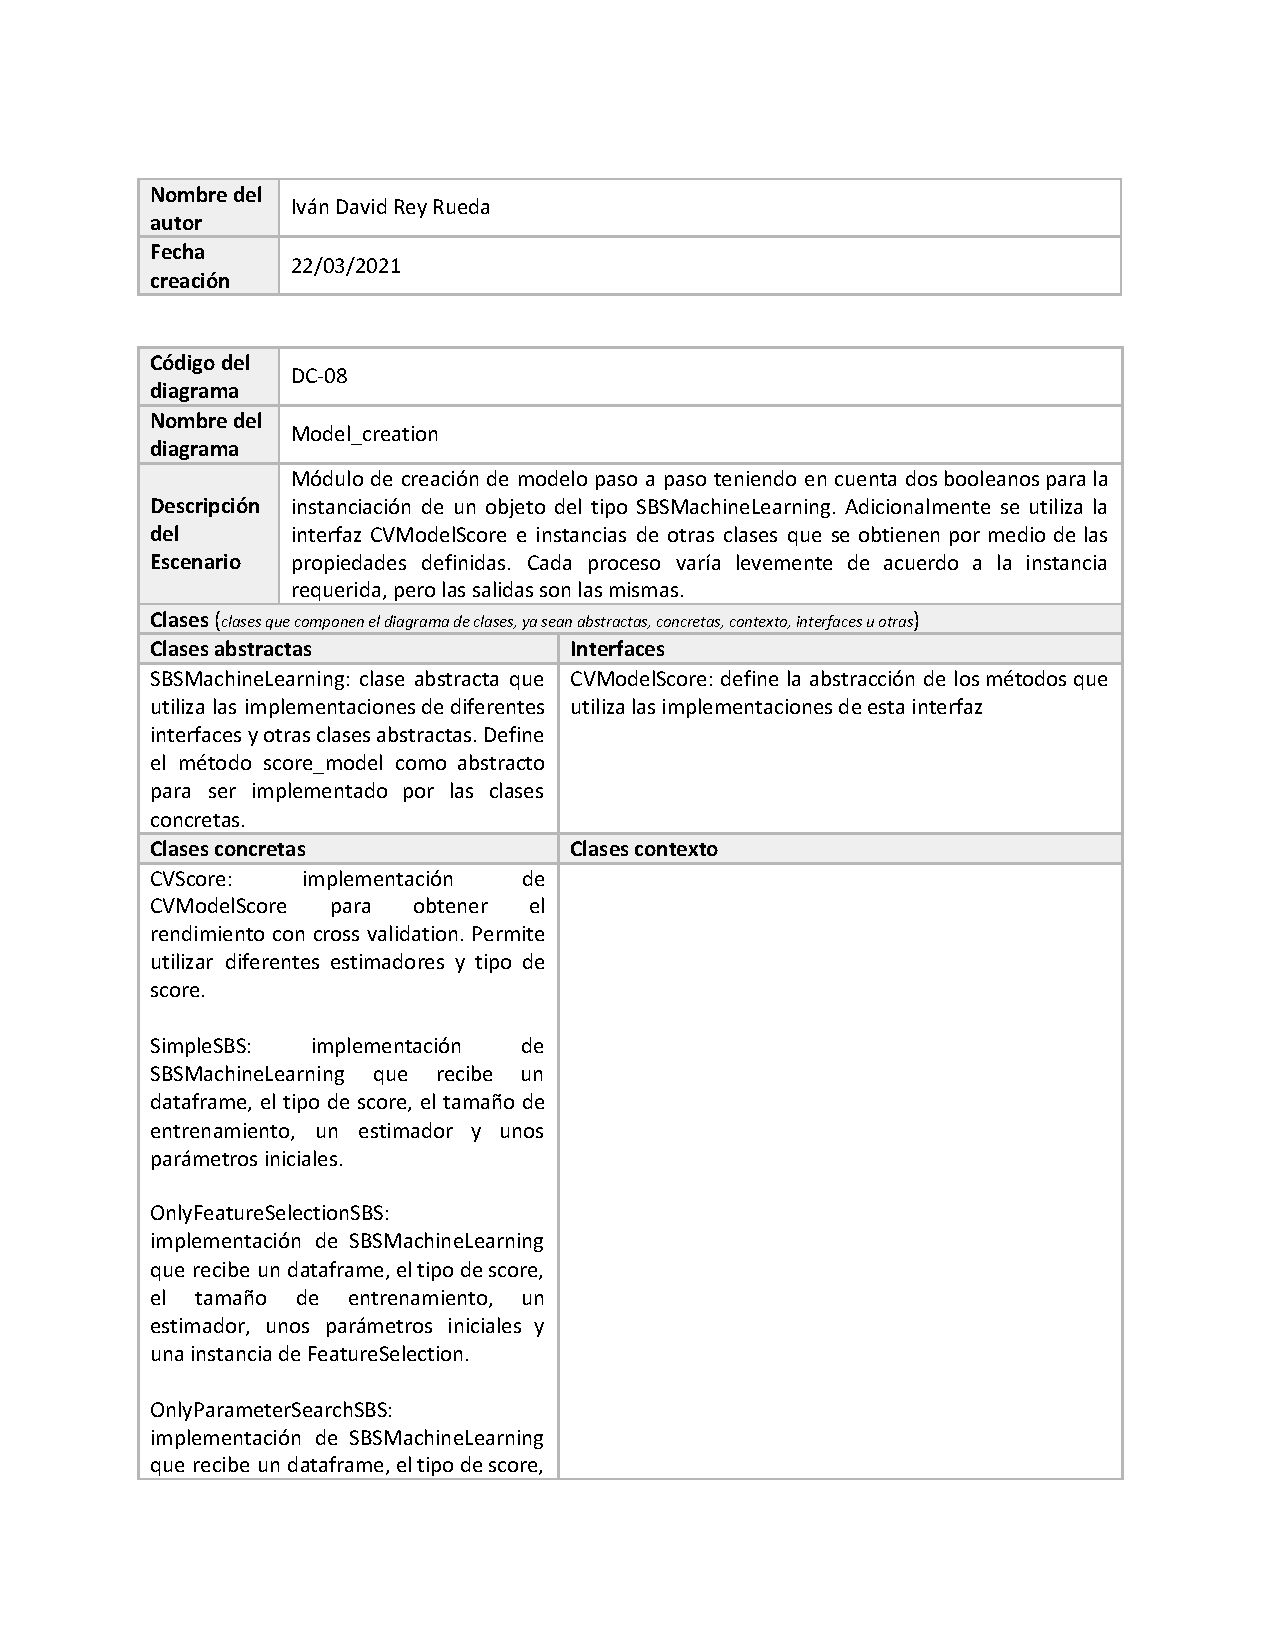
\includepdf[pages=-, pagecommand=\thispagestyle{otherplain}, width=\textwidth]{pdfs/Formato diagrama de clase DC-08_Firmado.pdf}
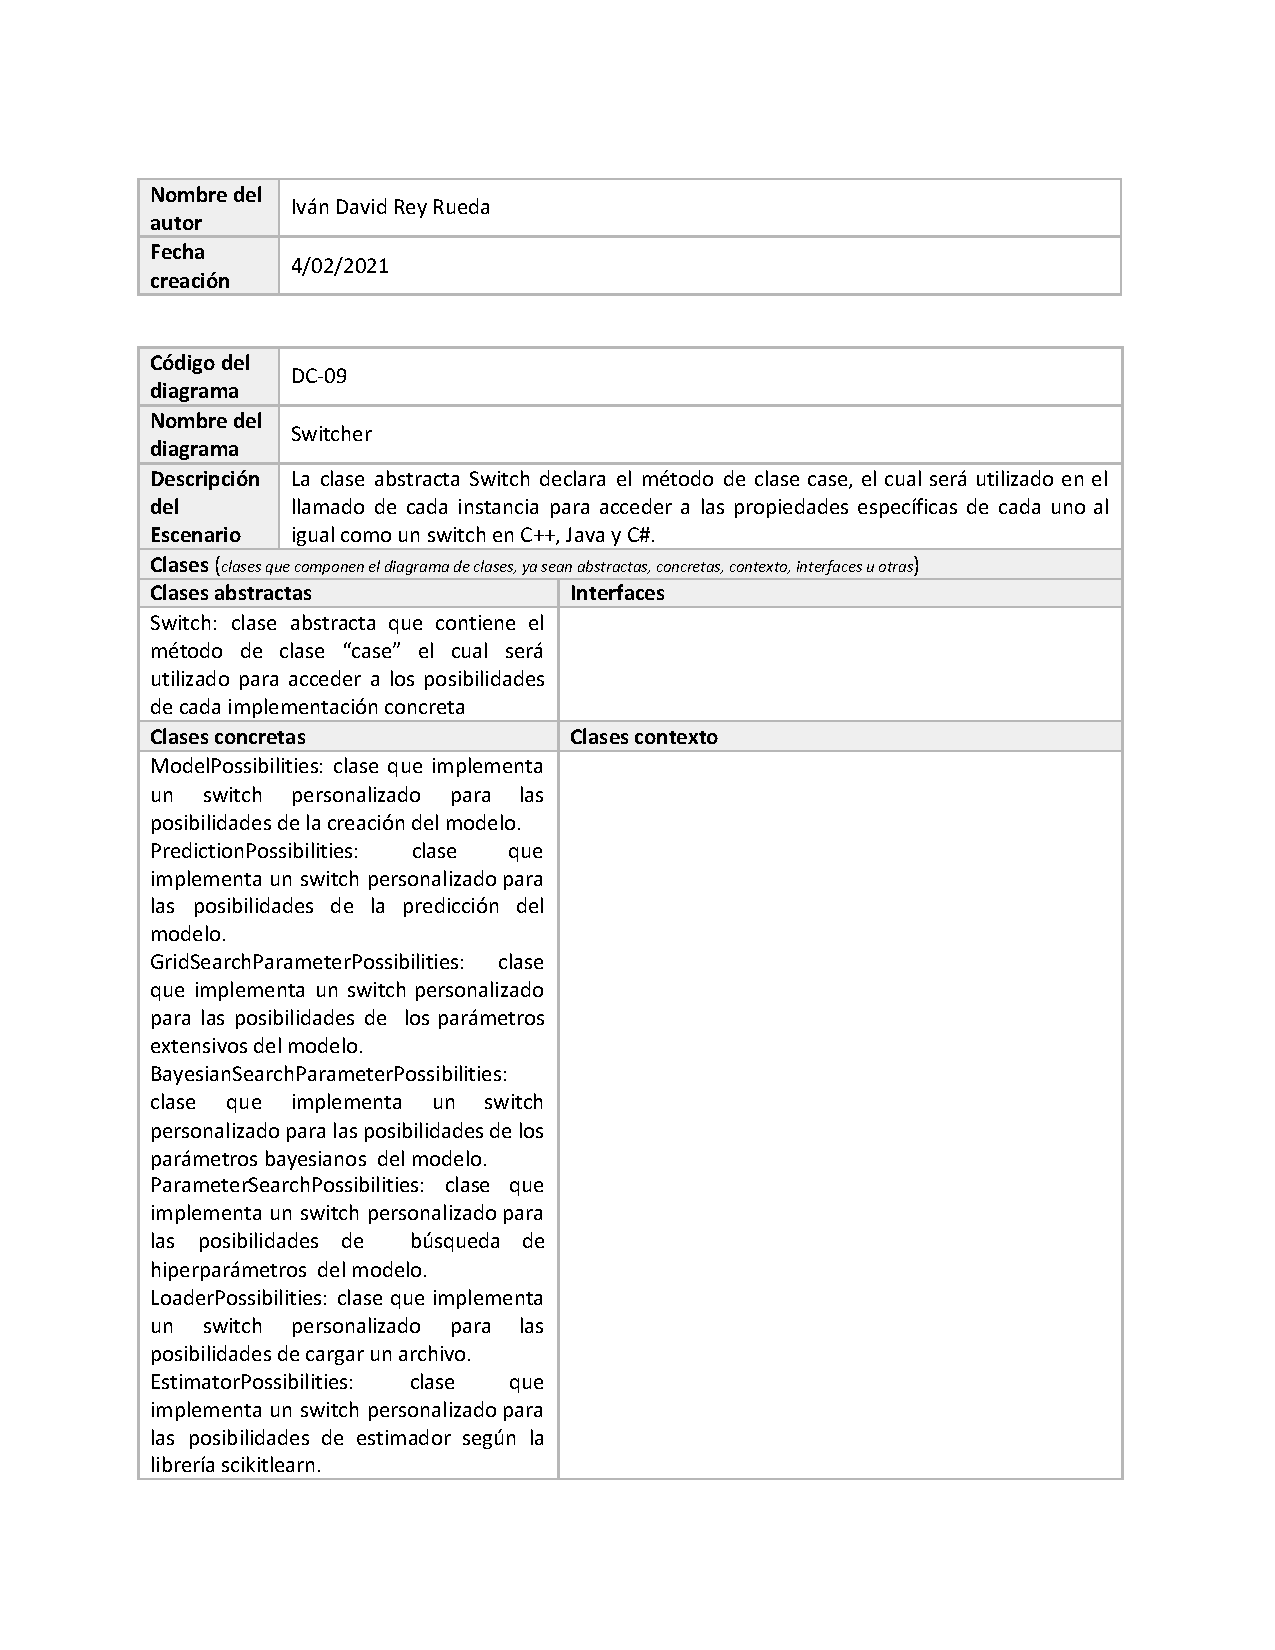
\includepdf[pages=-, pagecommand=\thispagestyle{otherplain}, width=\textwidth]{pdfs/Formato diagrama de clase DC-09_Firmado.pdf}
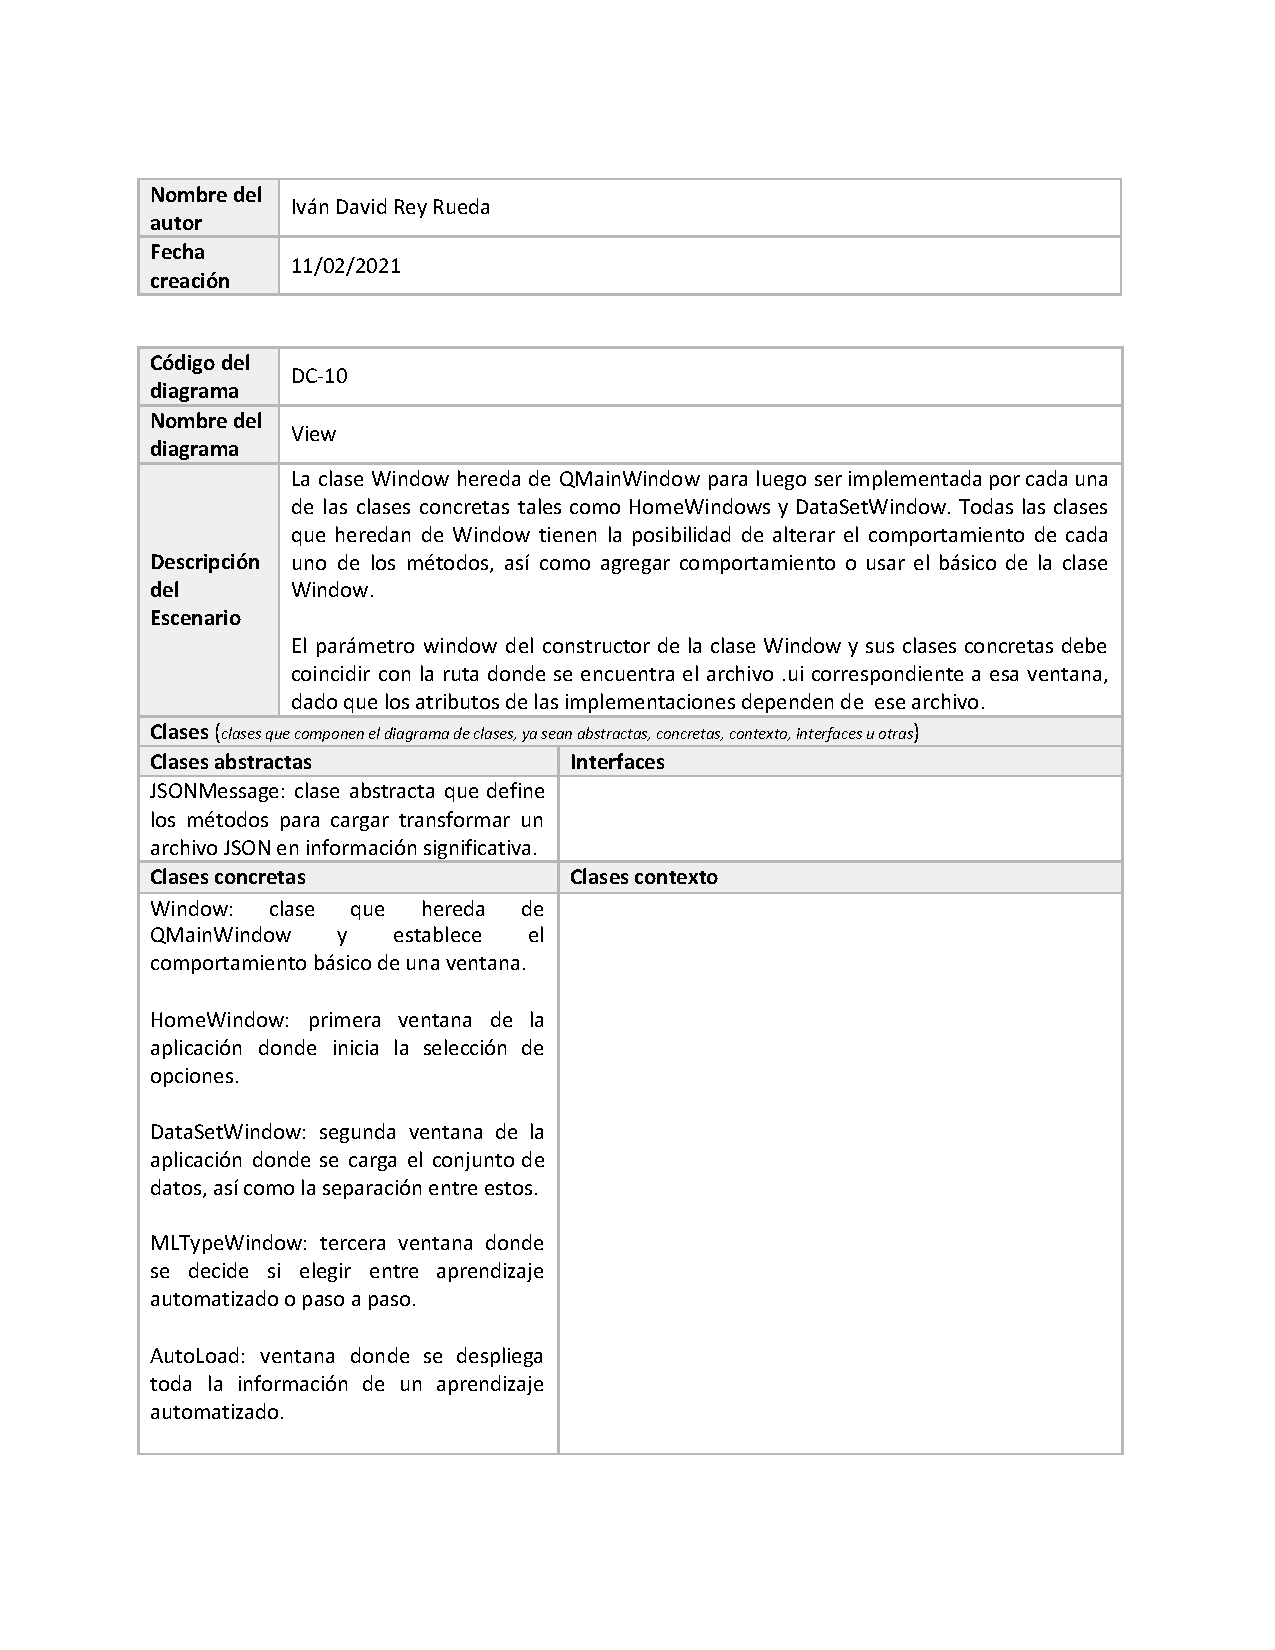
\includepdf[pages=-, pagecommand=\thispagestyle{otherplain}, width=\textwidth]{pdfs/Formato diagrama de clase DC-10_Firmado.pdf}
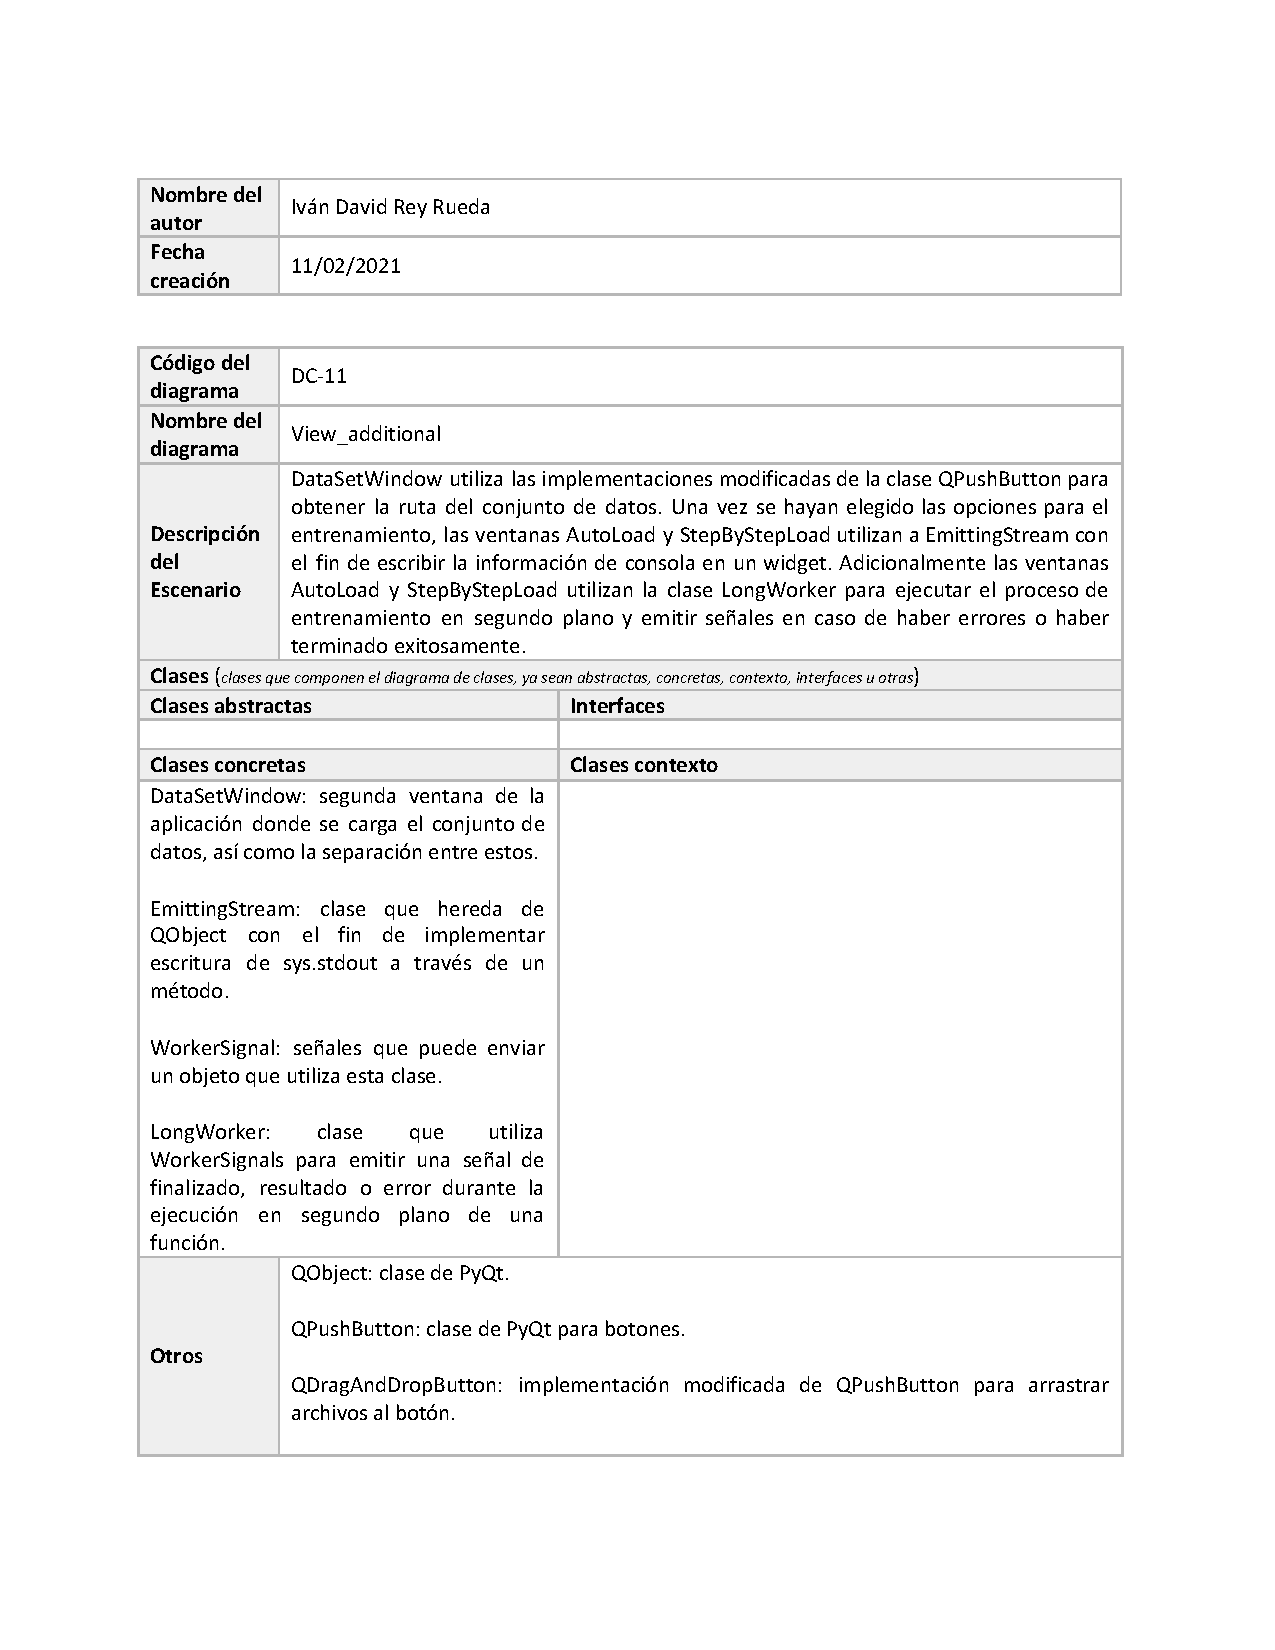
\includepdf[pages=-, pagecommand=\thispagestyle{otherplain}, width=\textwidth]{pdfs/Formato diagrama de clase DC-11_Firmado.pdf}
% casos de uso
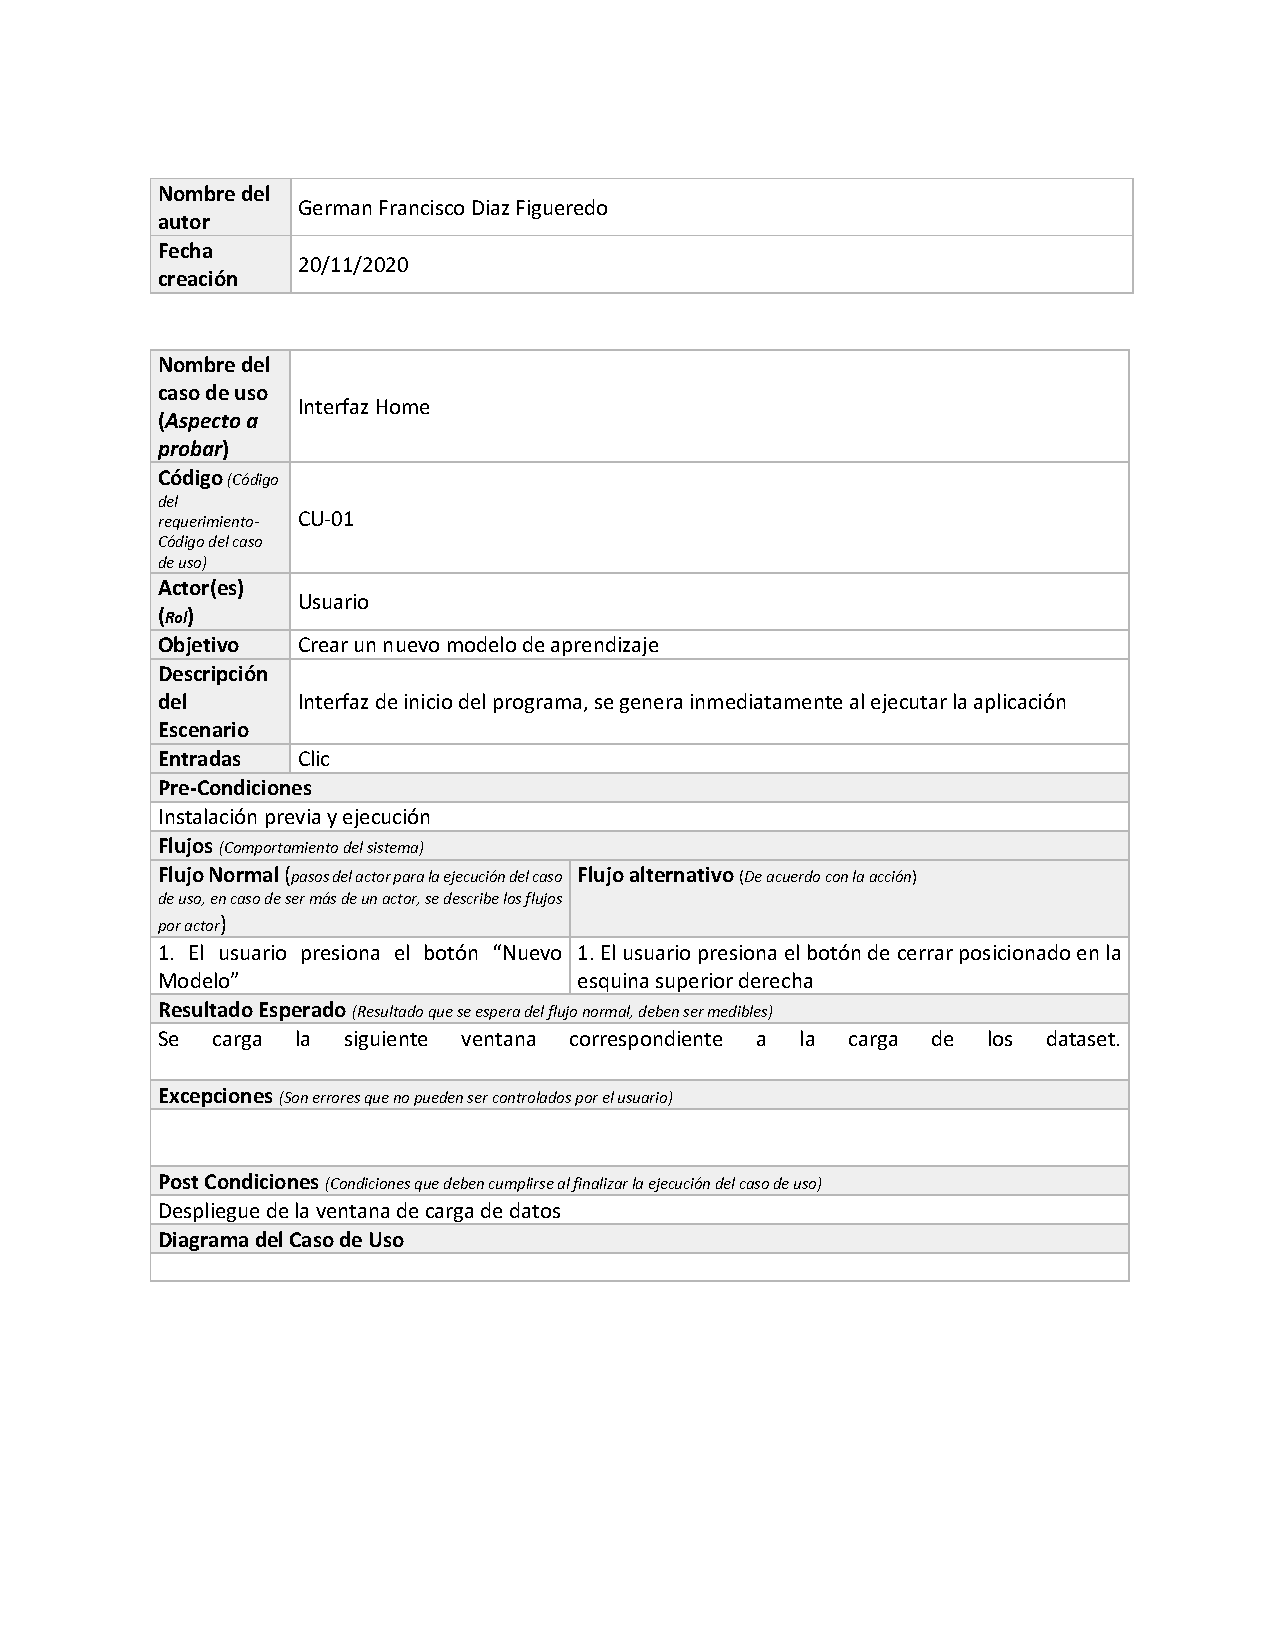
\includepdf[pages=-, pagecommand=\thispagestyle{otherplain}, width=\textwidth]{pdfs/CU-01_Firmado.pdf}
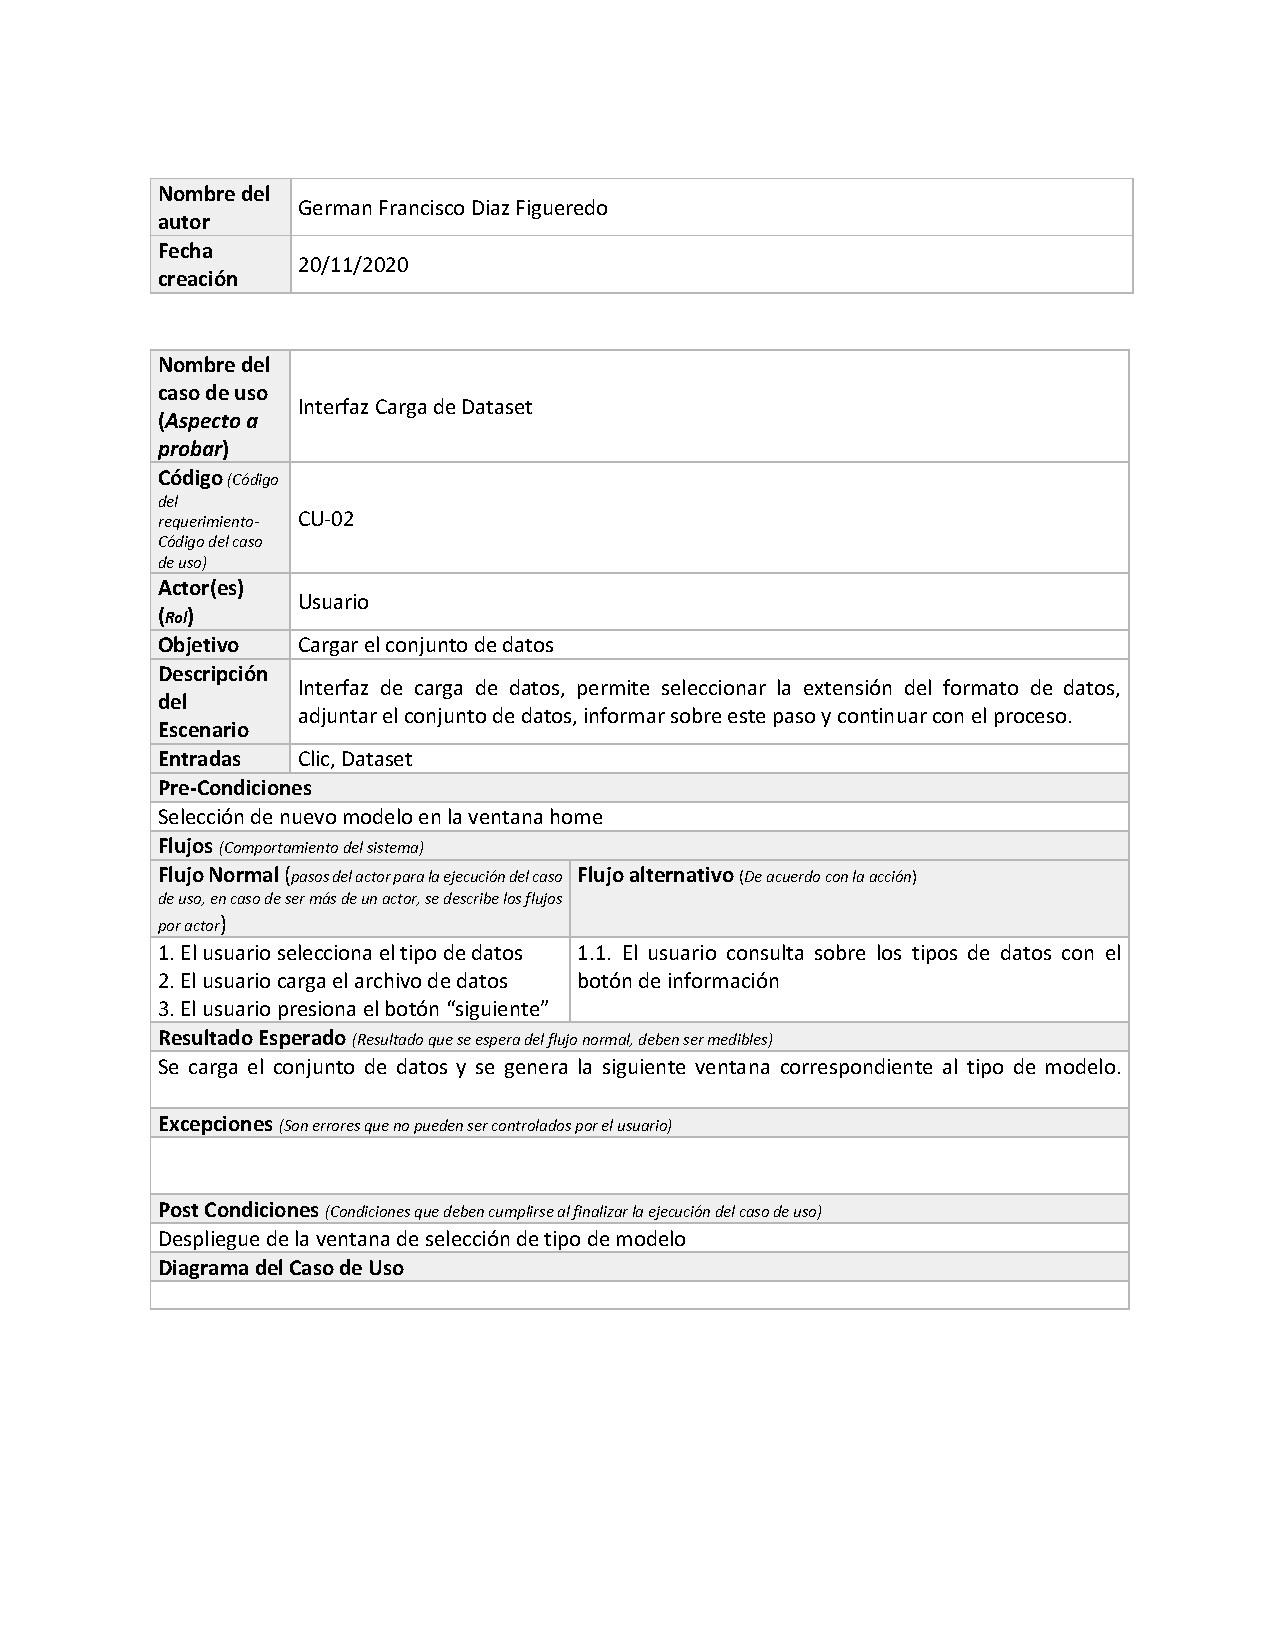
\includepdf[pages=-, pagecommand=\thispagestyle{otherplain}, width=\textwidth]{pdfs/CU-02_Firmado.pdf}
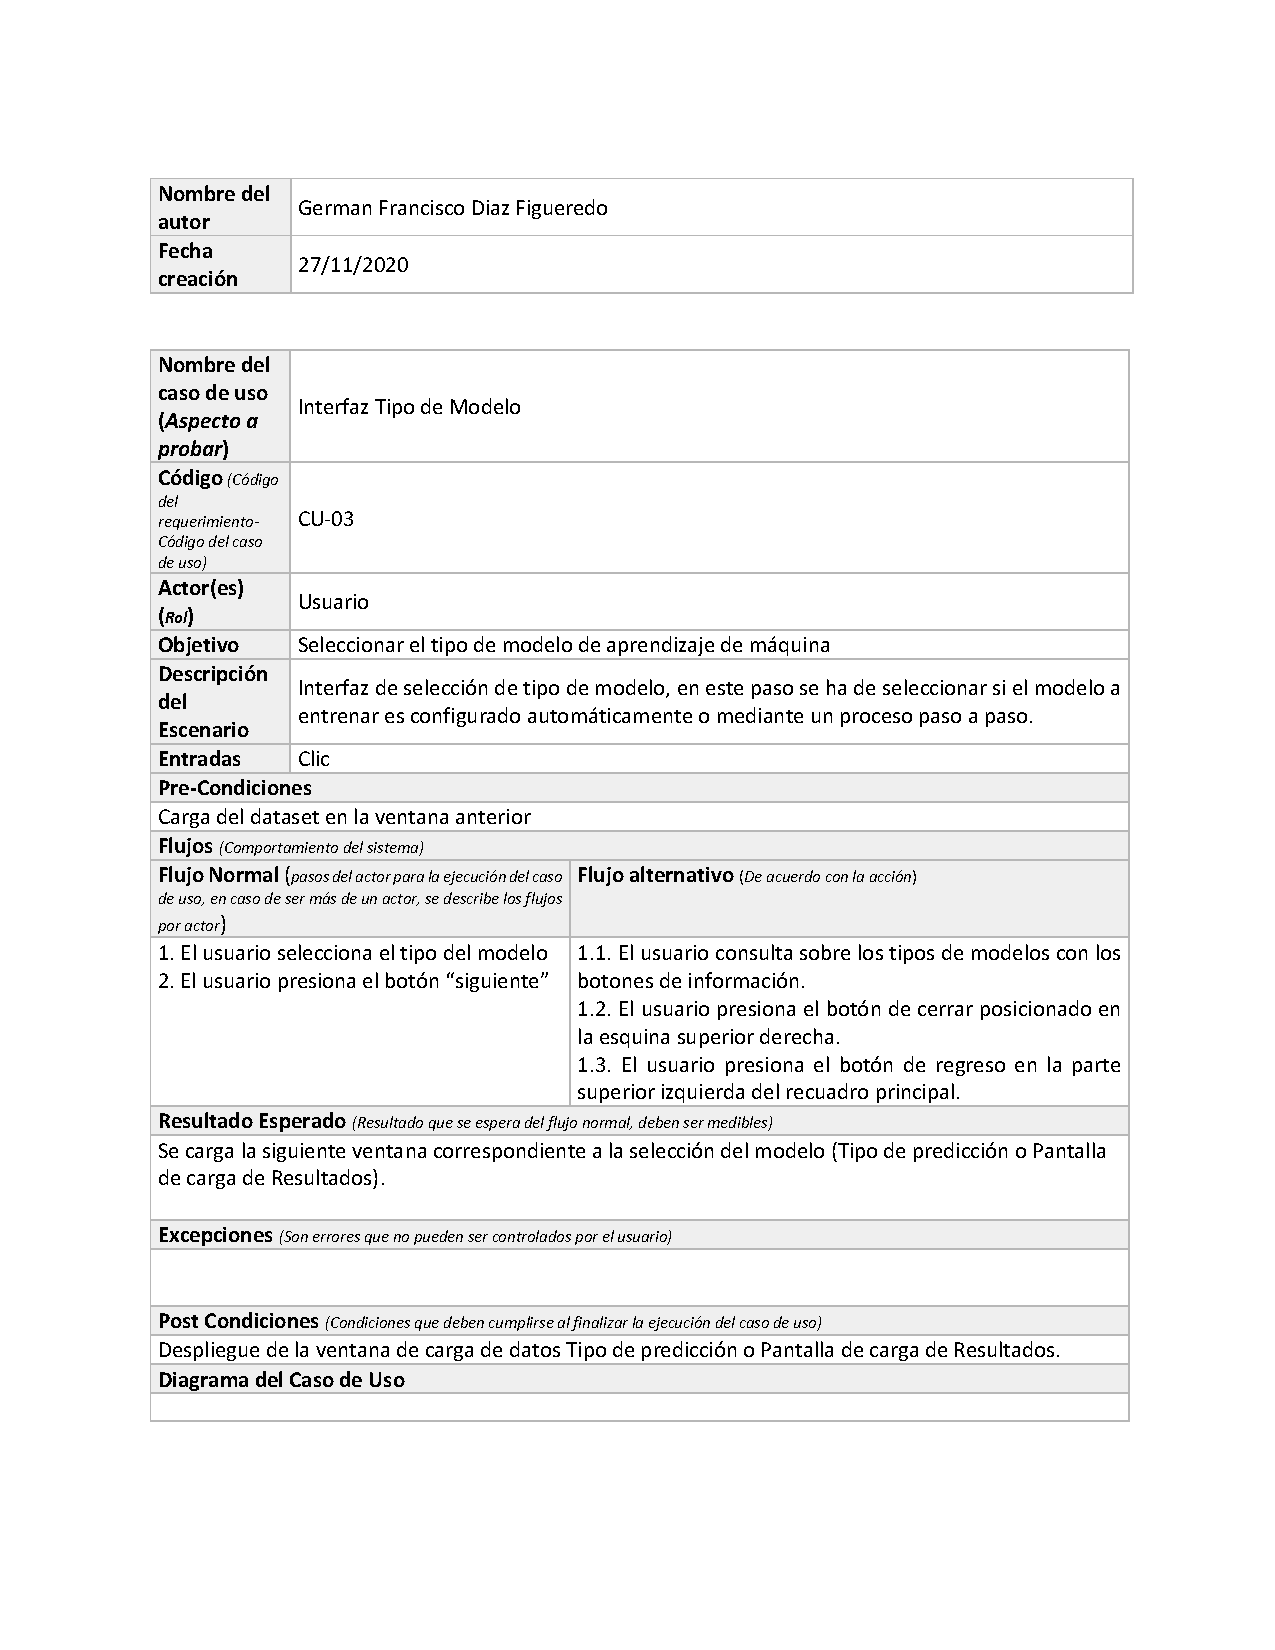
\includepdf[pages=-, pagecommand=\thispagestyle{otherplain}, width=\textwidth]{pdfs/CU-03_Firmado.pdf}
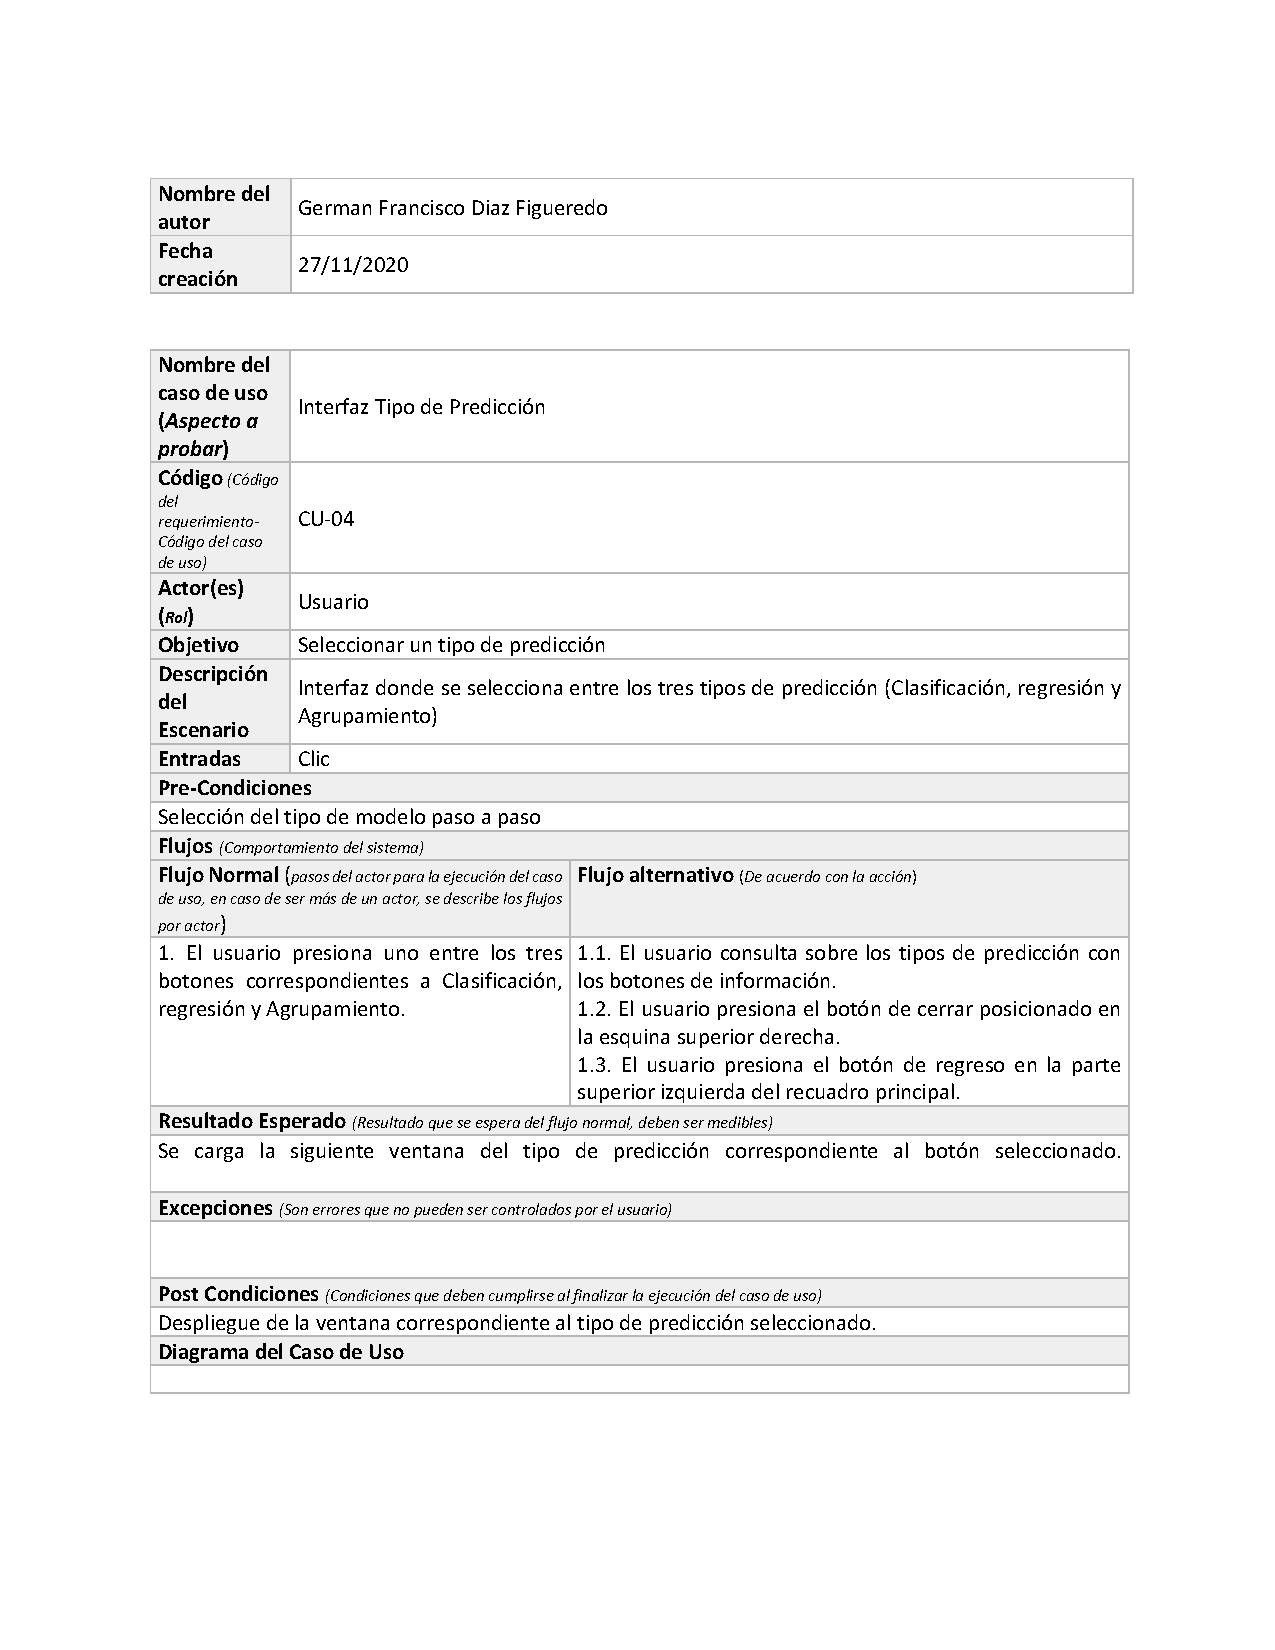
\includepdf[pages=-, pagecommand=\thispagestyle{otherplain}, width=\textwidth]{pdfs/CU-04_Firmado.pdf}
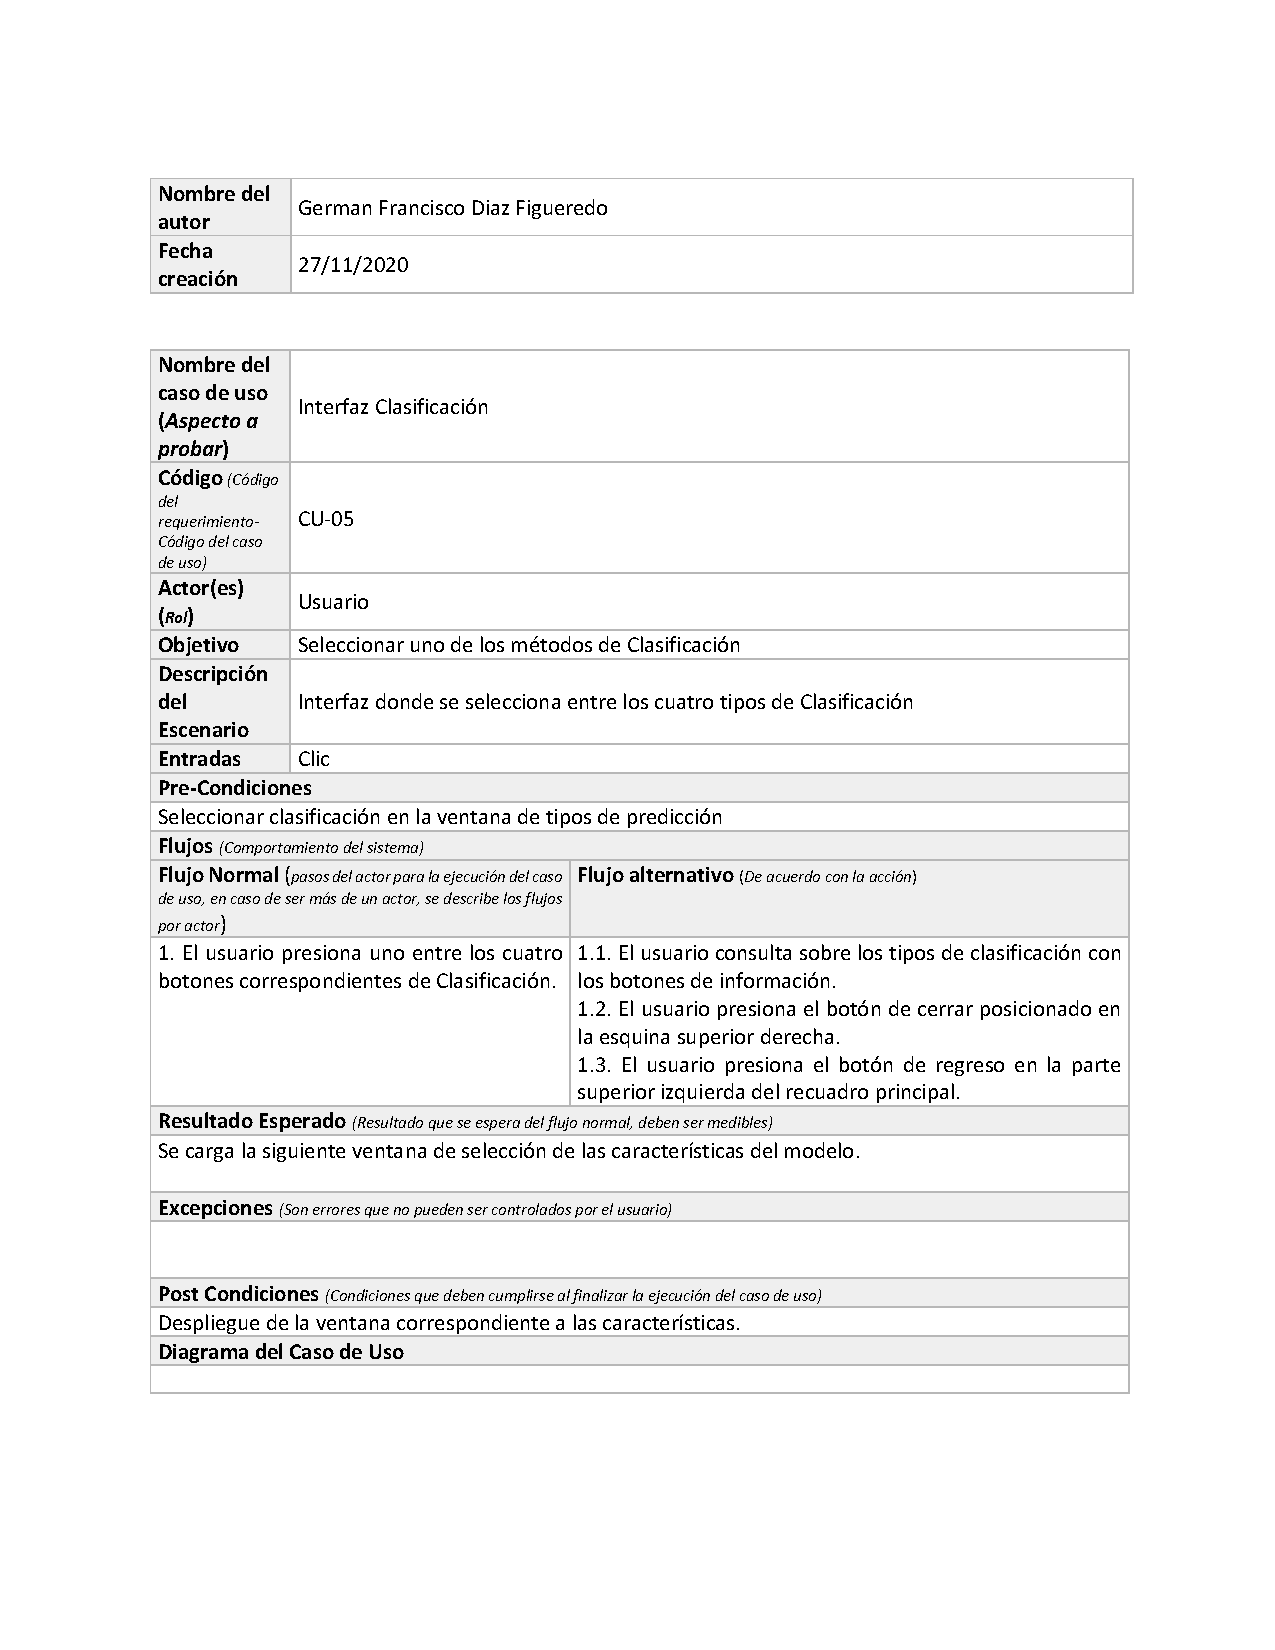
\includepdf[pages=-, pagecommand=\thispagestyle{otherplain}, width=\textwidth]{pdfs/CU-05_Firmado.pdf}
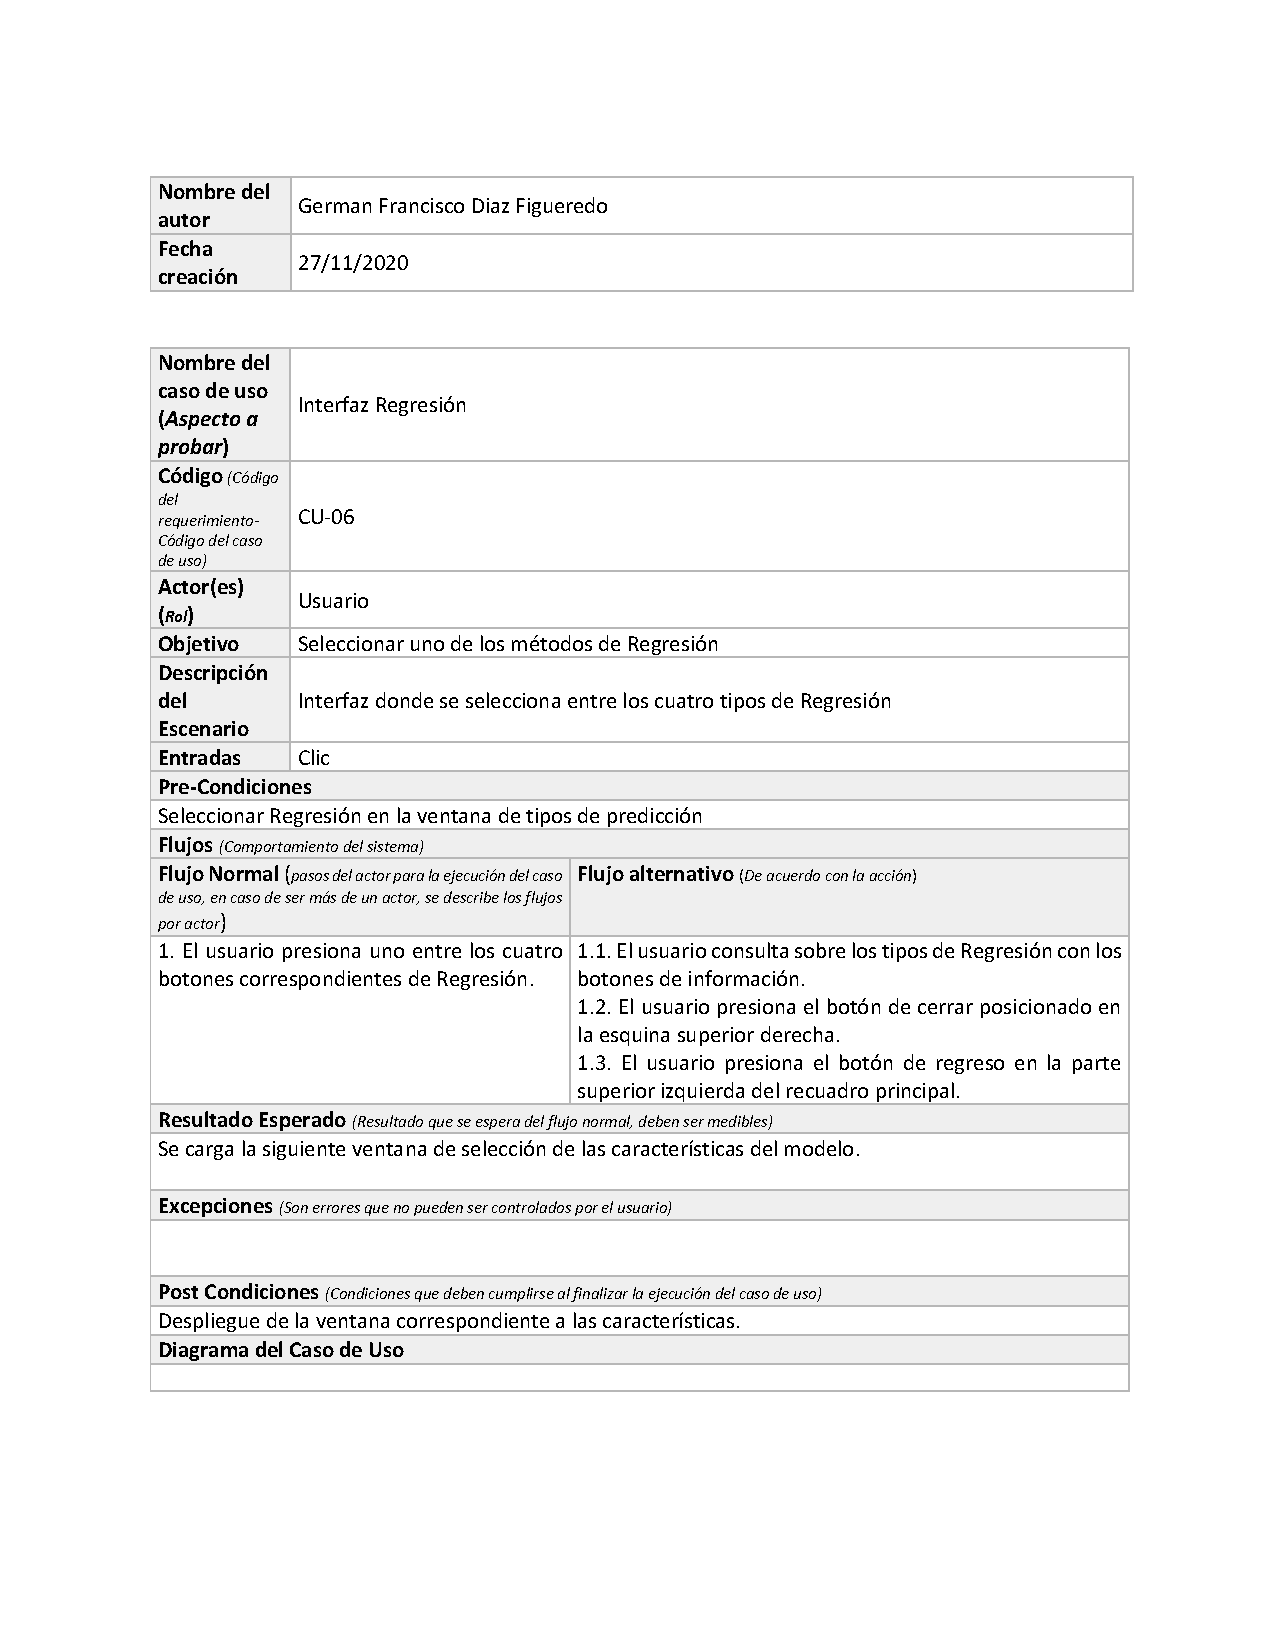
\includepdf[pages=-, pagecommand=\thispagestyle{otherplain}, width=\textwidth]{pdfs/CU-06_Firmado.pdf}
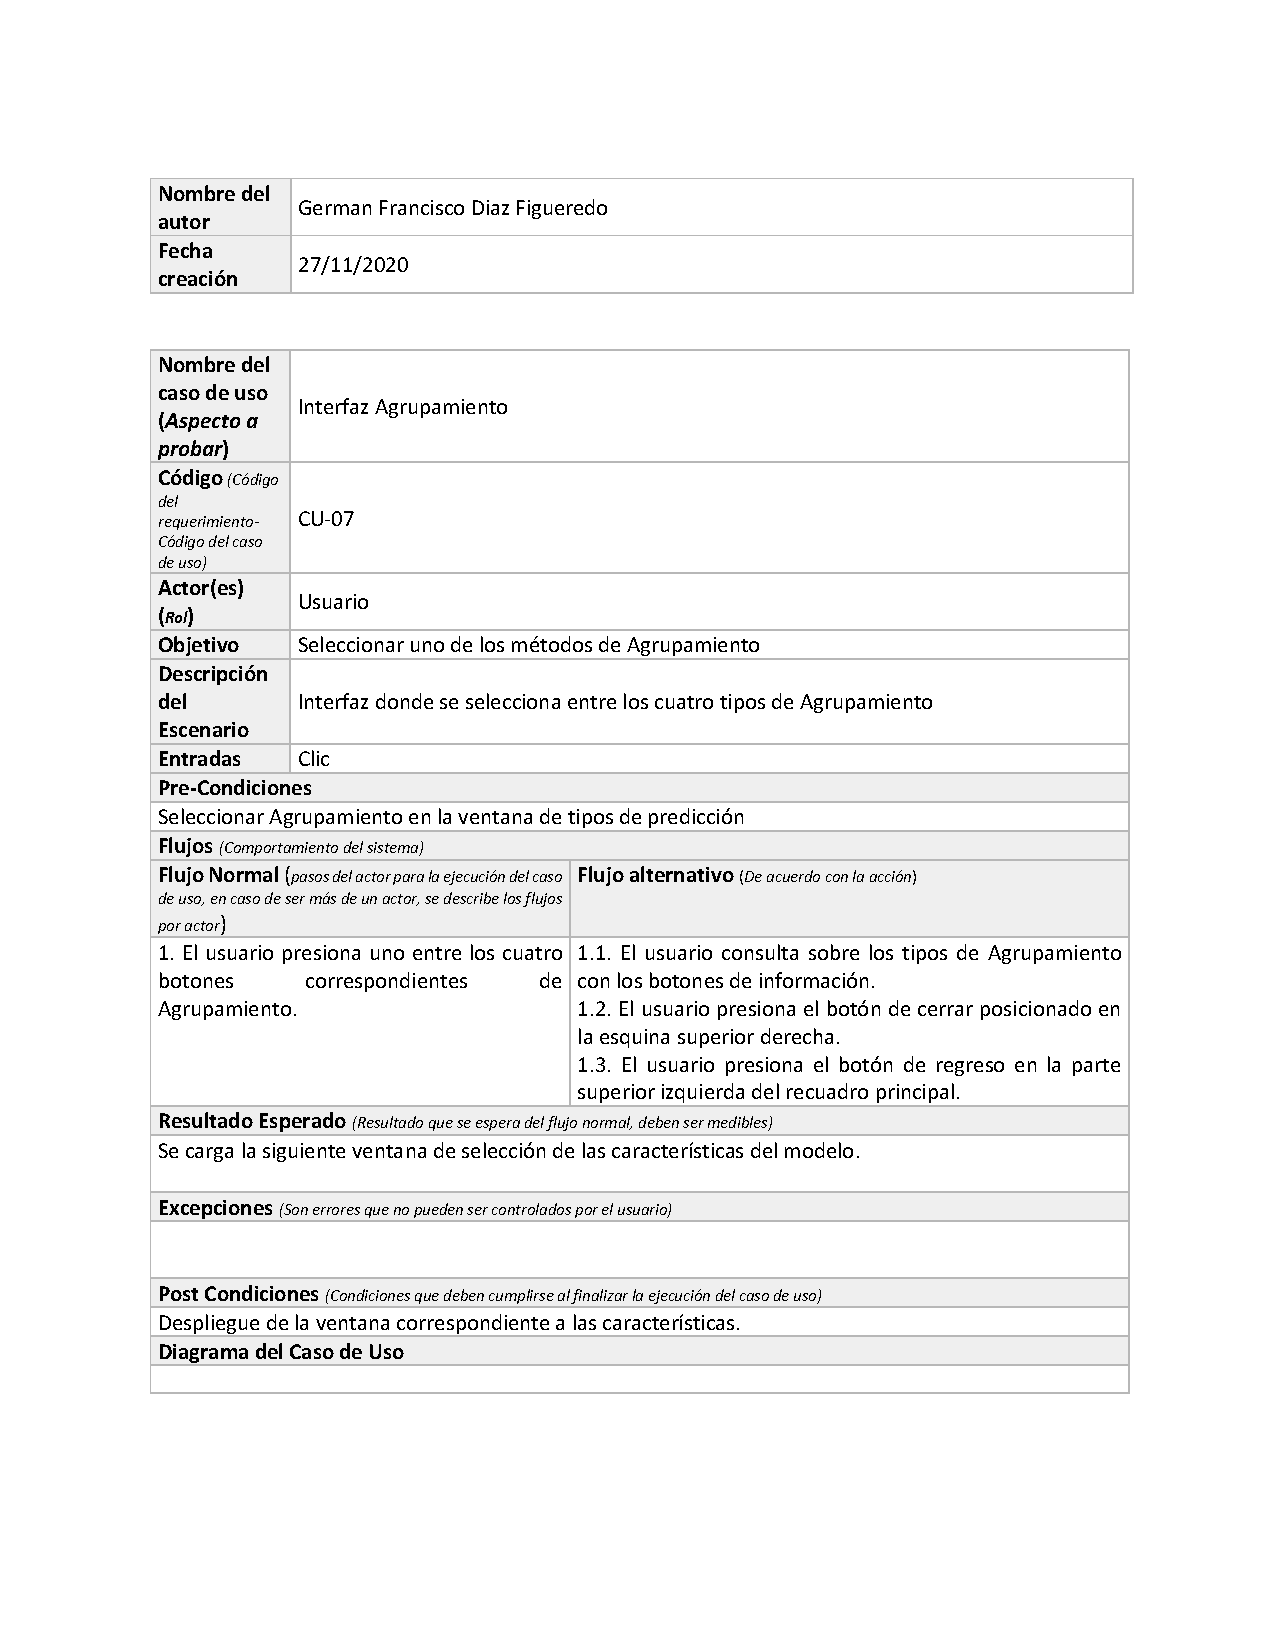
\includepdf[pages=-, pagecommand=\thispagestyle{otherplain}, width=\textwidth]{pdfs/CU-07_Firmado.pdf}
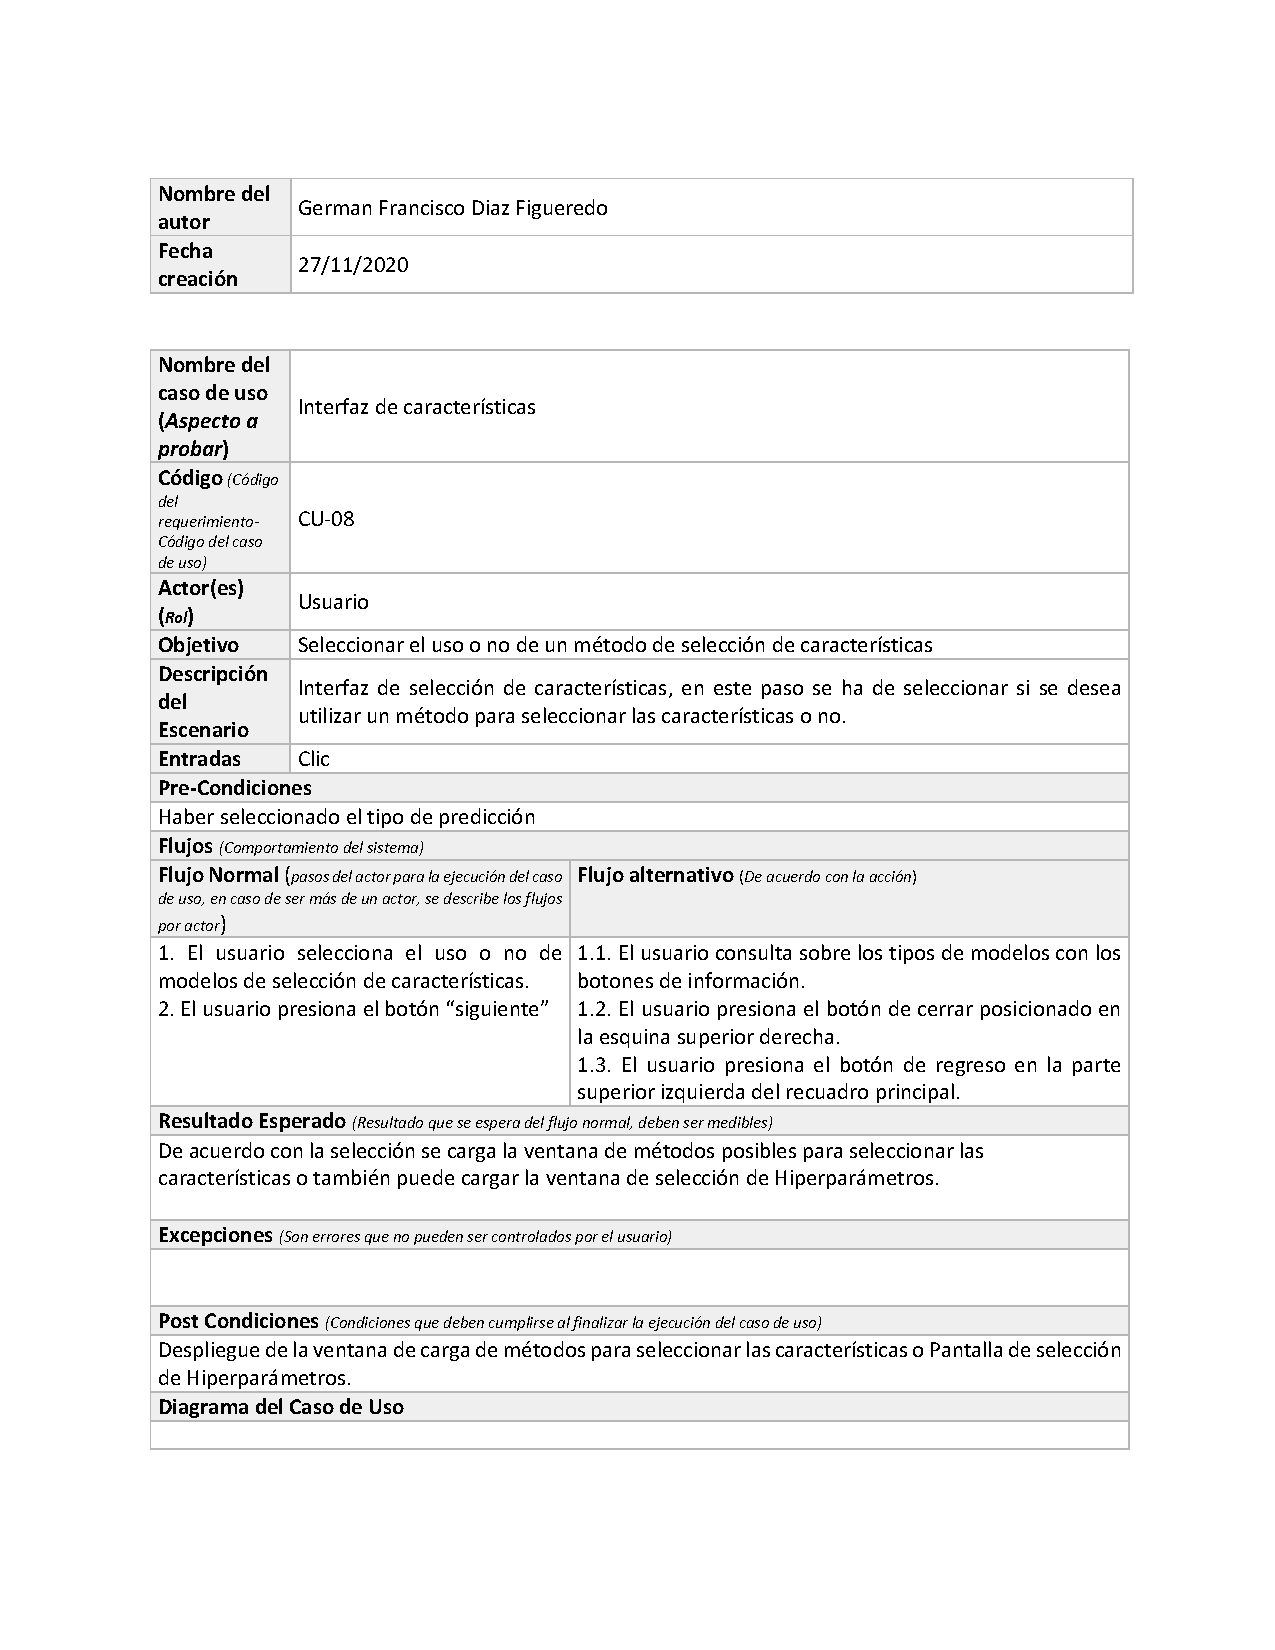
\includepdf[pages=-, pagecommand=\thispagestyle{otherplain}, width=\textwidth]{pdfs/CU-08_Firmado.pdf}
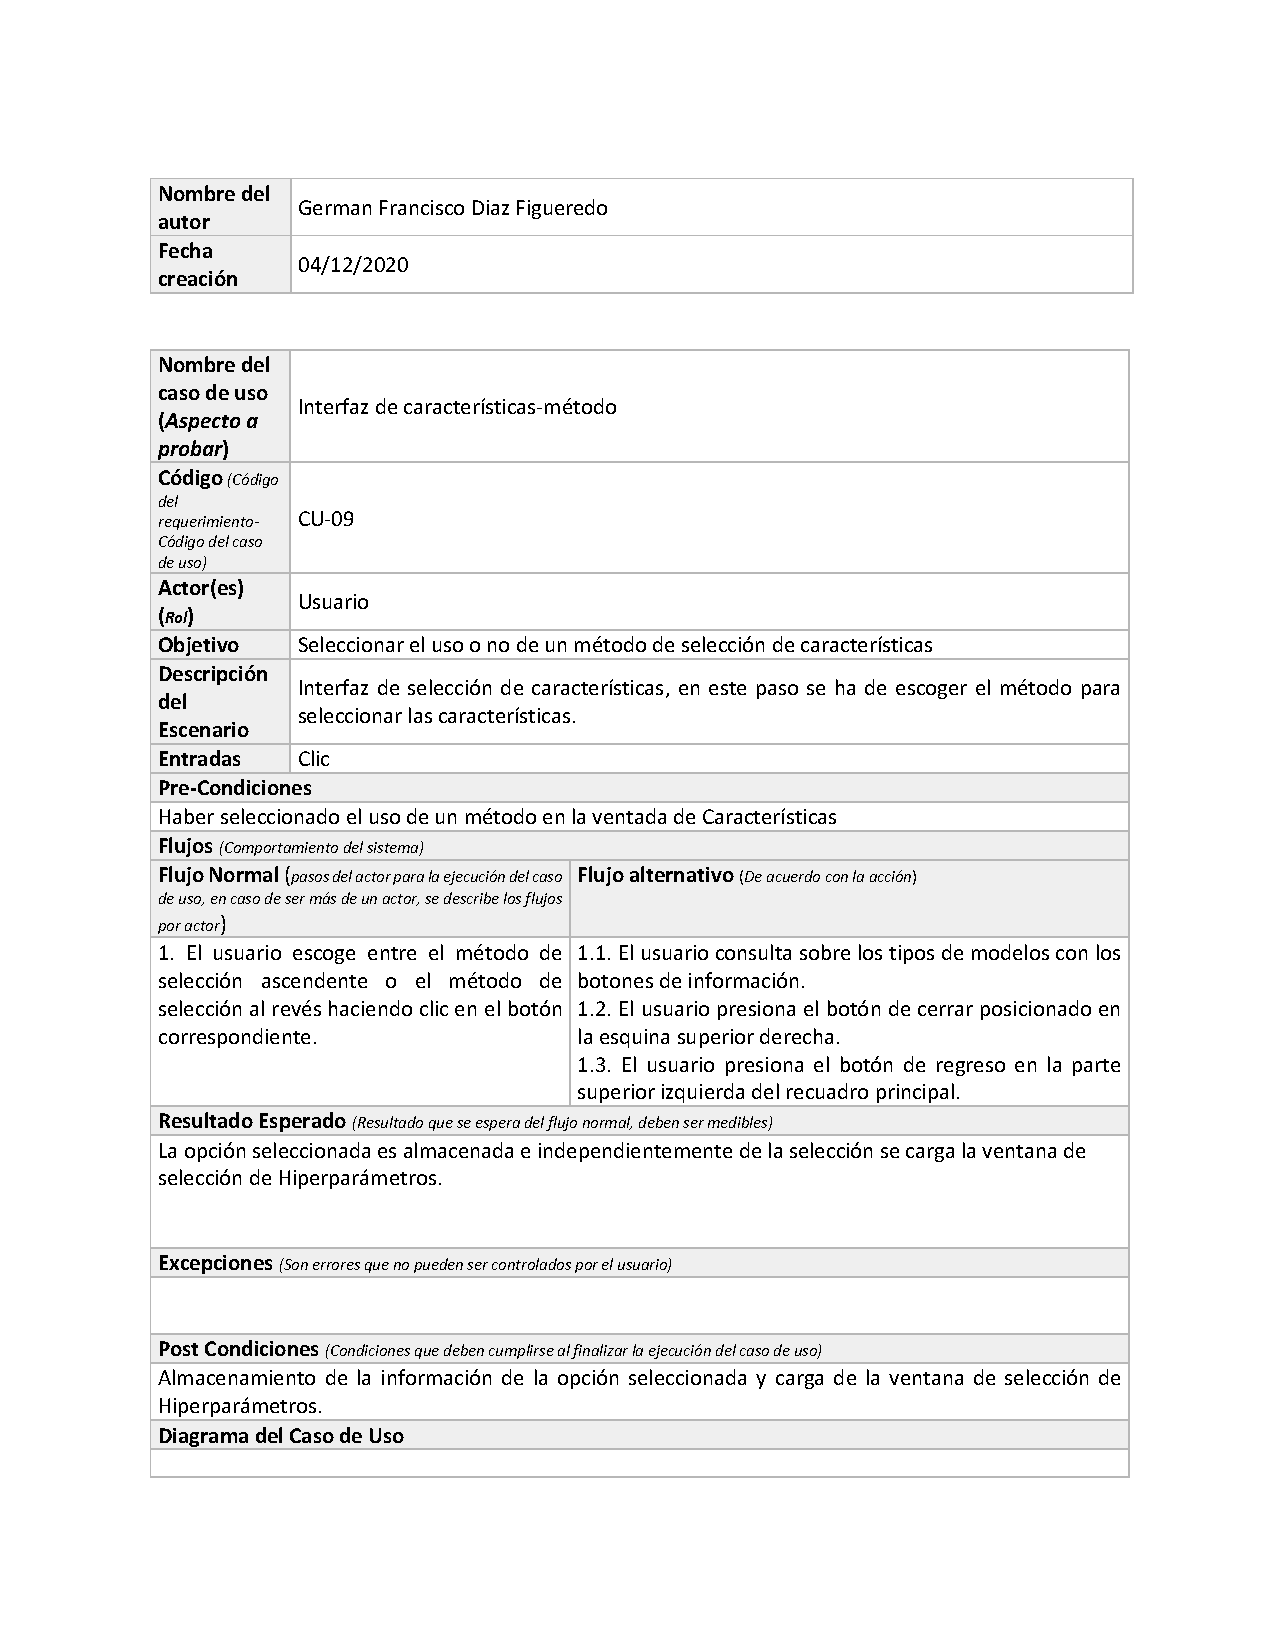
\includepdf[pages=-, pagecommand=\thispagestyle{otherplain}, width=\textwidth]{pdfs/CU-09_Firmado.pdf}
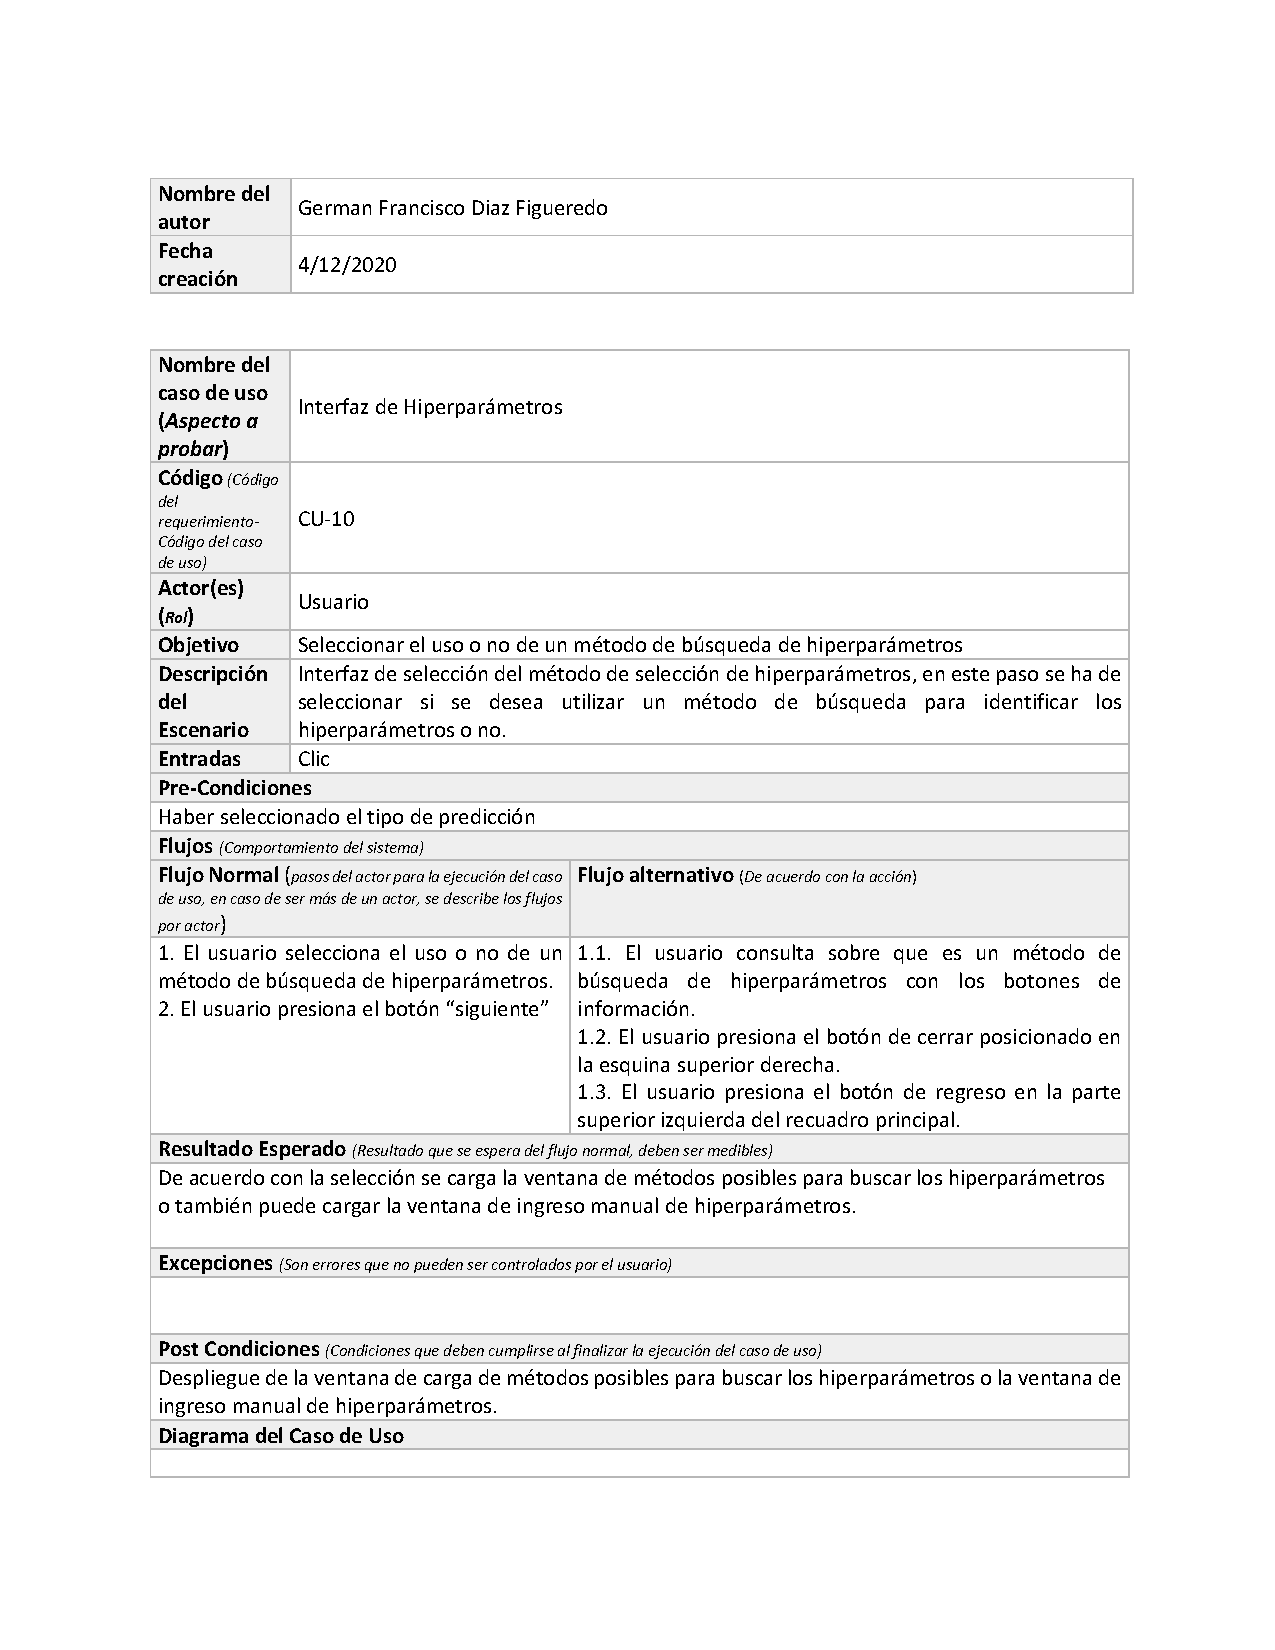
\includepdf[pages=-, pagecommand=\thispagestyle{otherplain}, width=\textwidth]{pdfs/CU-10_Firmado.pdf}
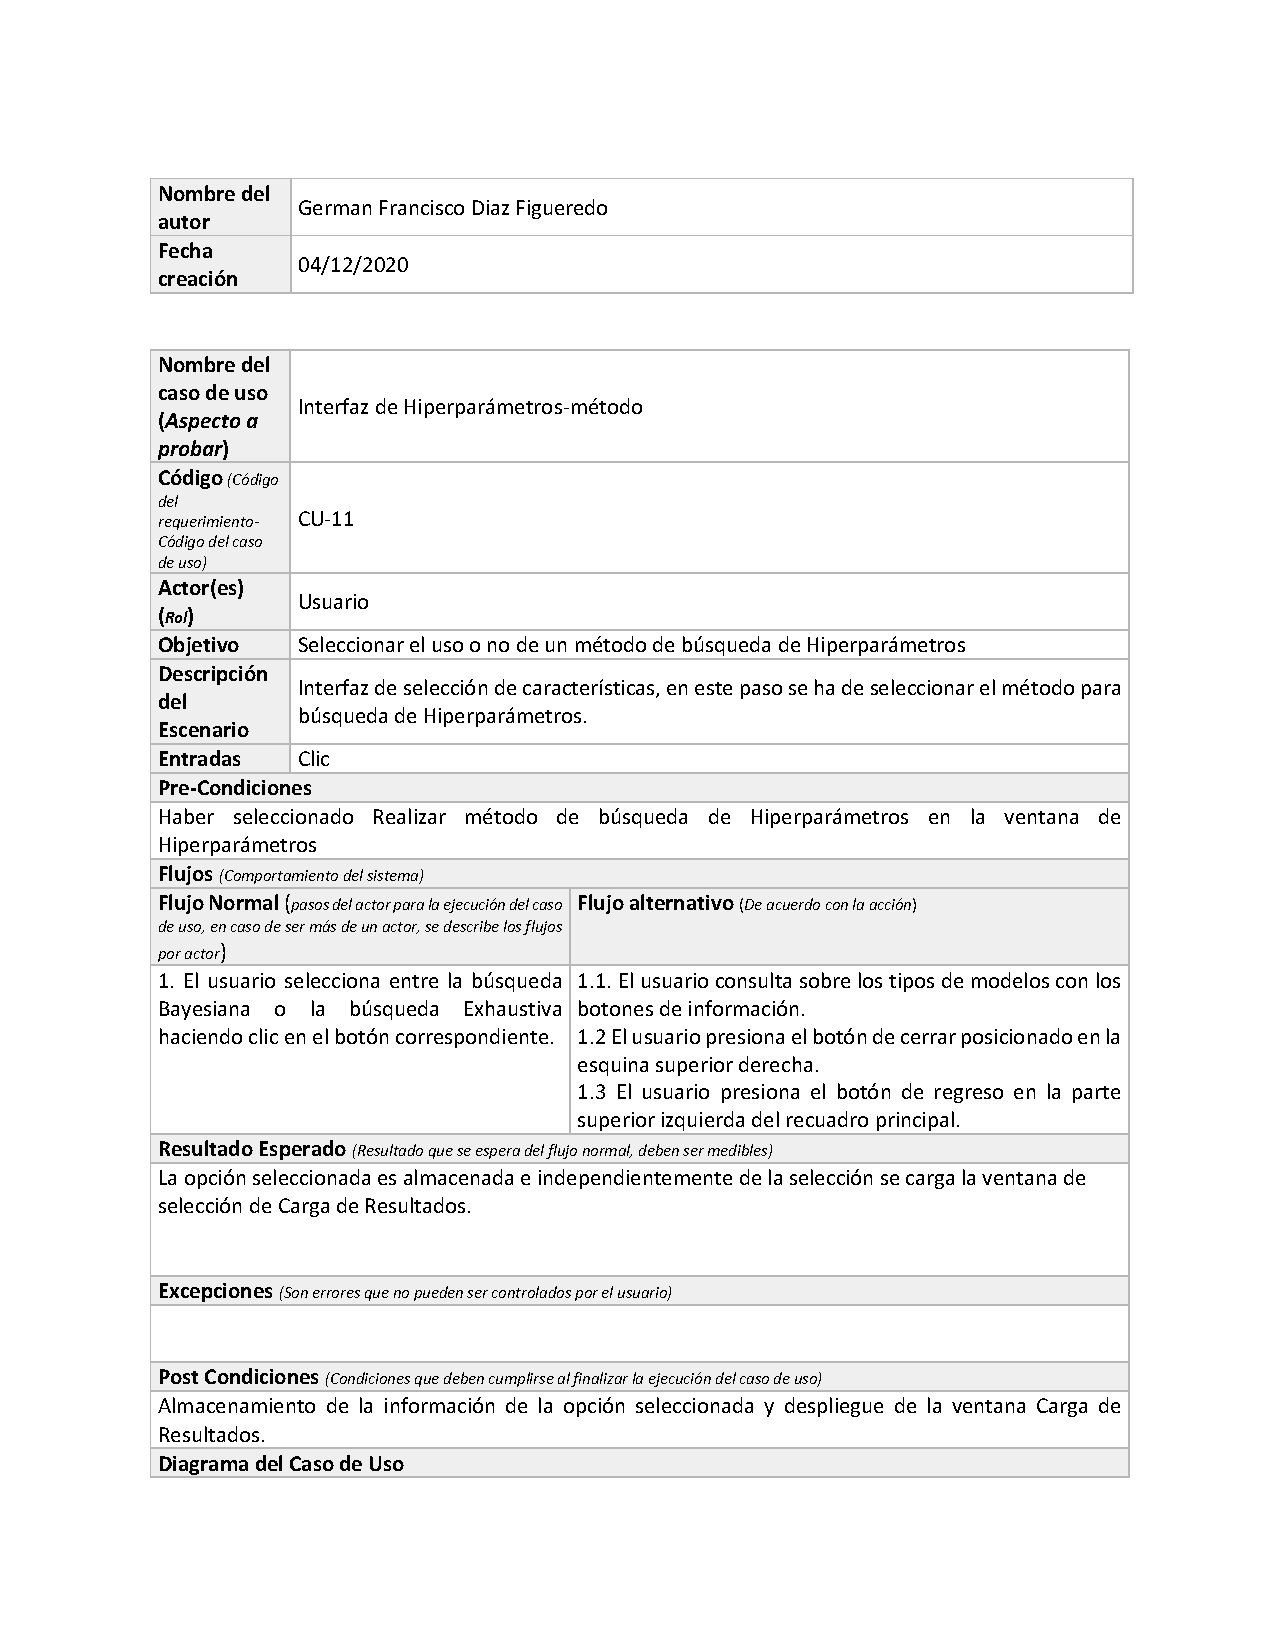
\includepdf[pages=-, pagecommand=\thispagestyle{otherplain}, width=\textwidth]{pdfs/CU-11_Firmado.pdf}
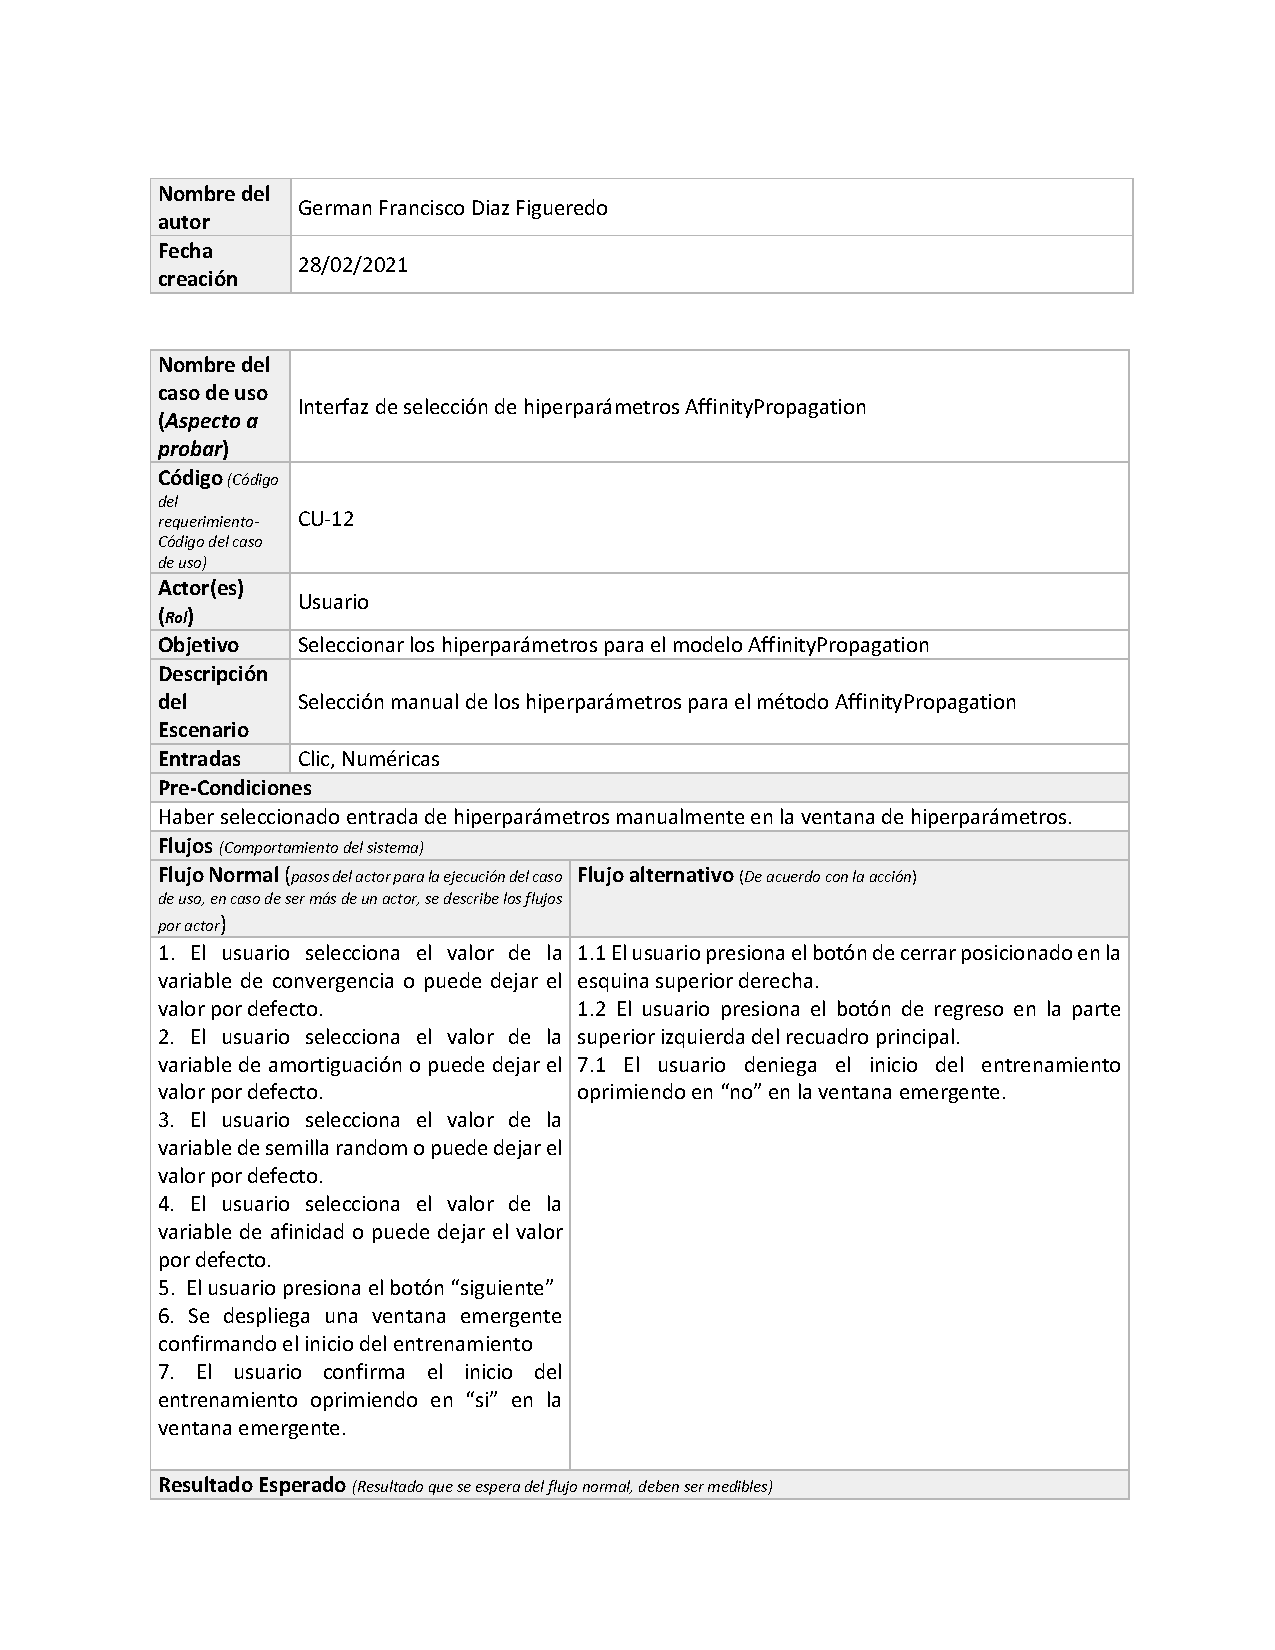
\includepdf[pages=-, pagecommand=\thispagestyle{otherplain}, width=\textwidth]{pdfs/CU-12_Firmado.pdf}
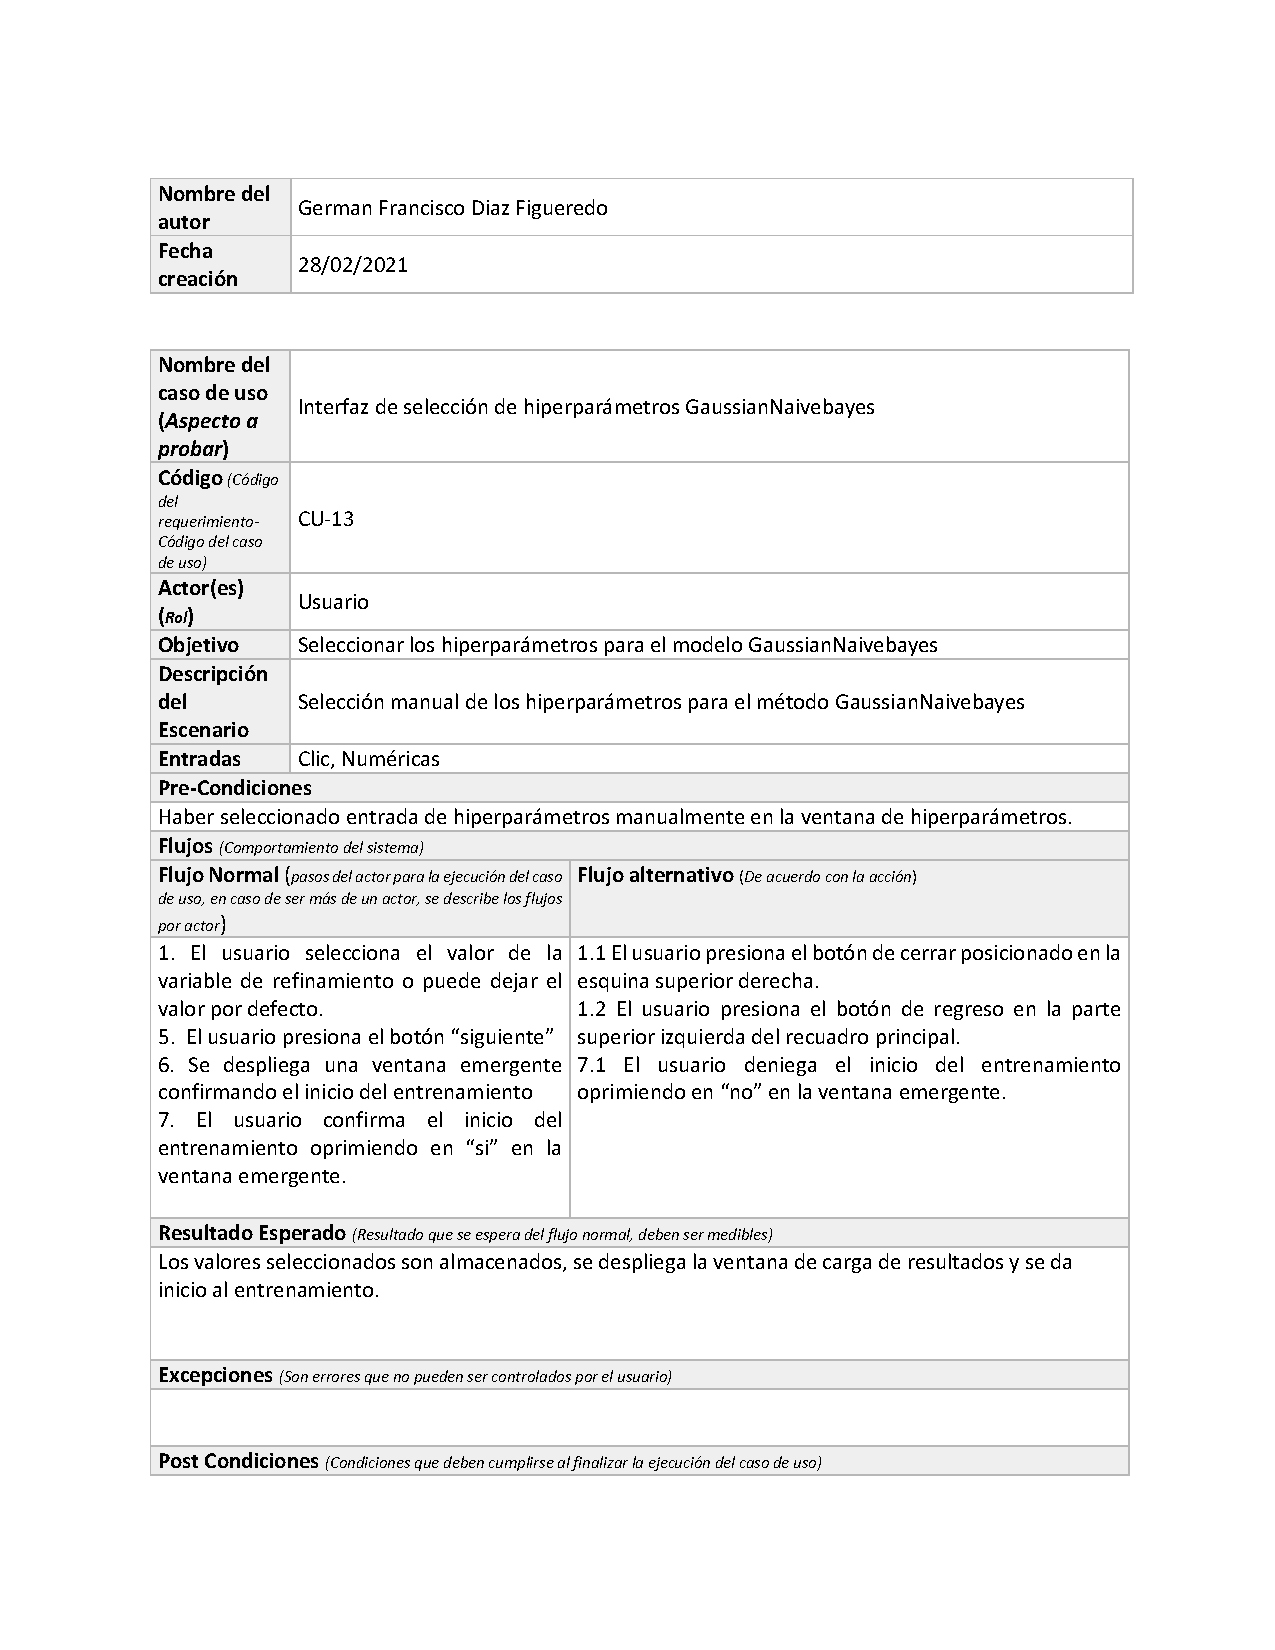
\includepdf[pages=-, pagecommand=\thispagestyle{otherplain}, width=\textwidth]{pdfs/CU-13_Firmado.pdf}
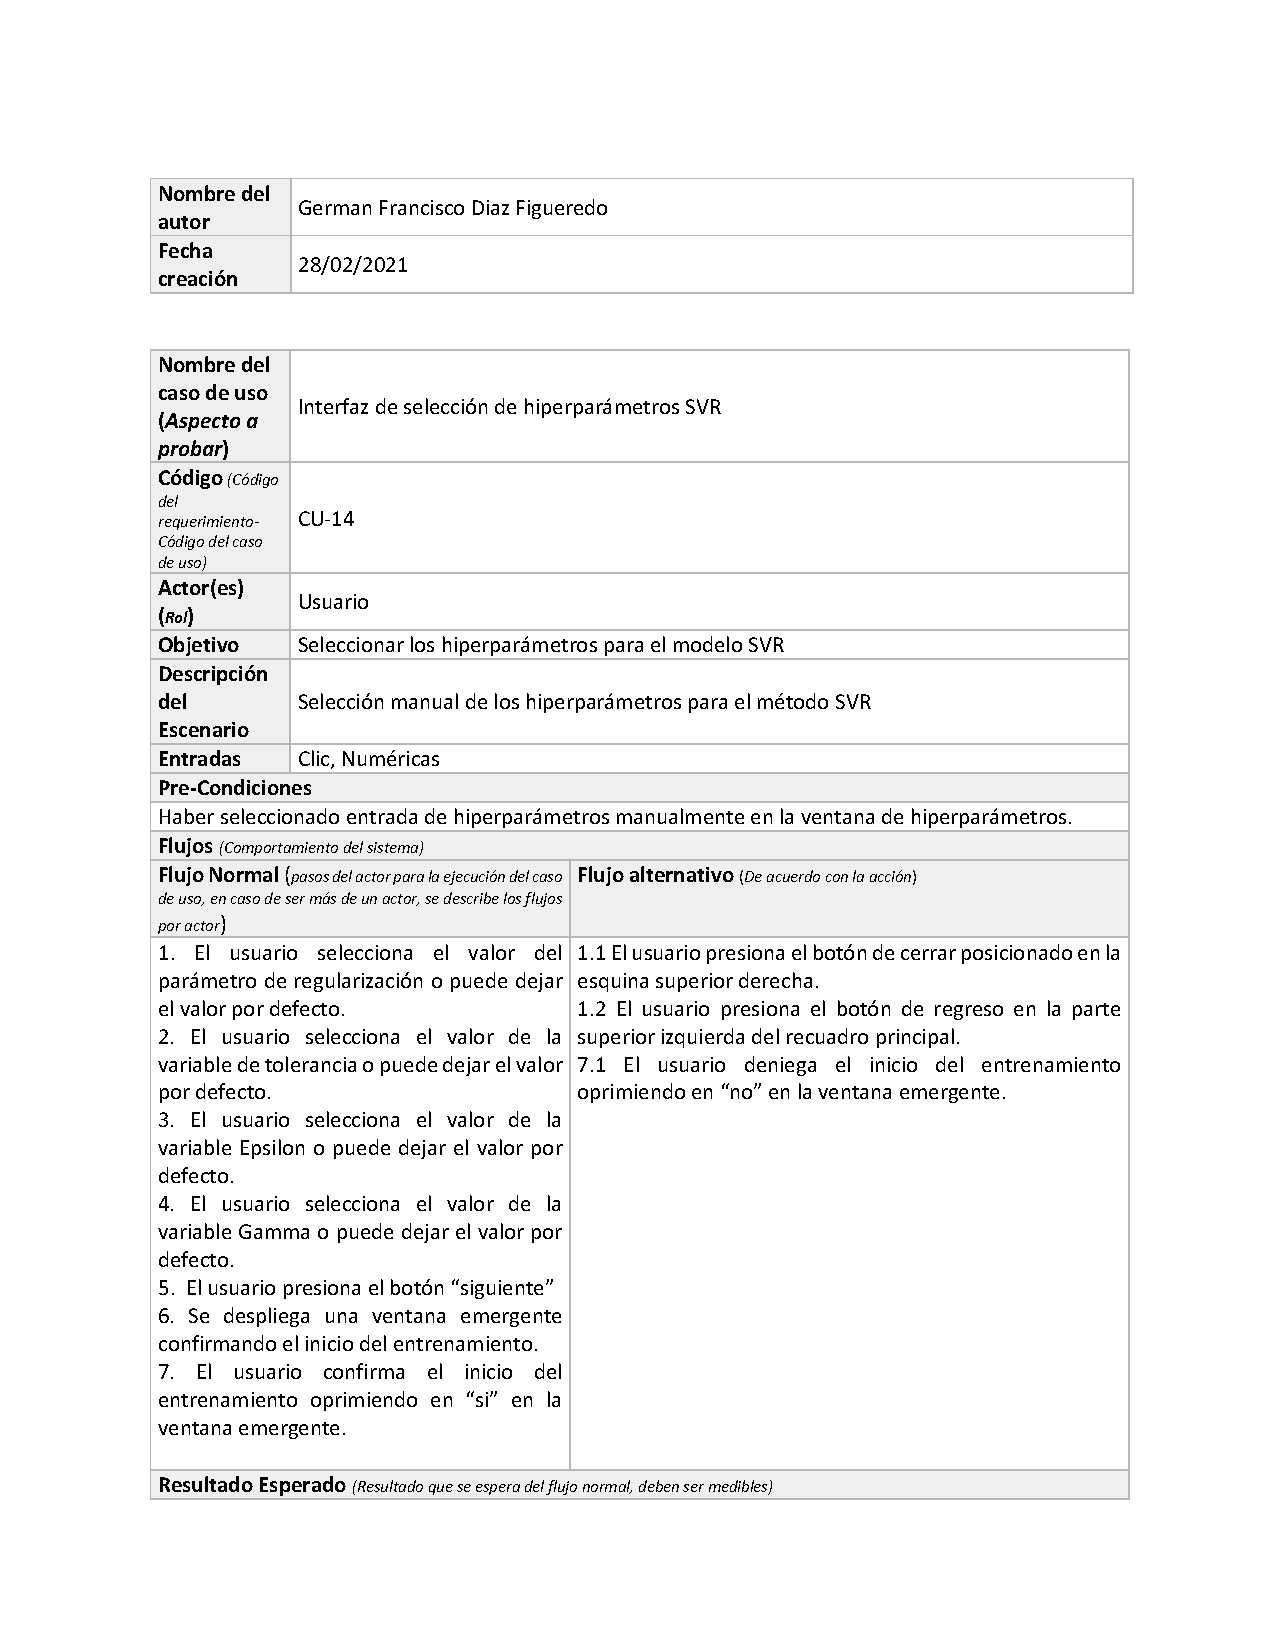
\includepdf[pages=-, pagecommand=\thispagestyle{otherplain}, width=\textwidth]{pdfs/CU-14_Firmado.pdf}
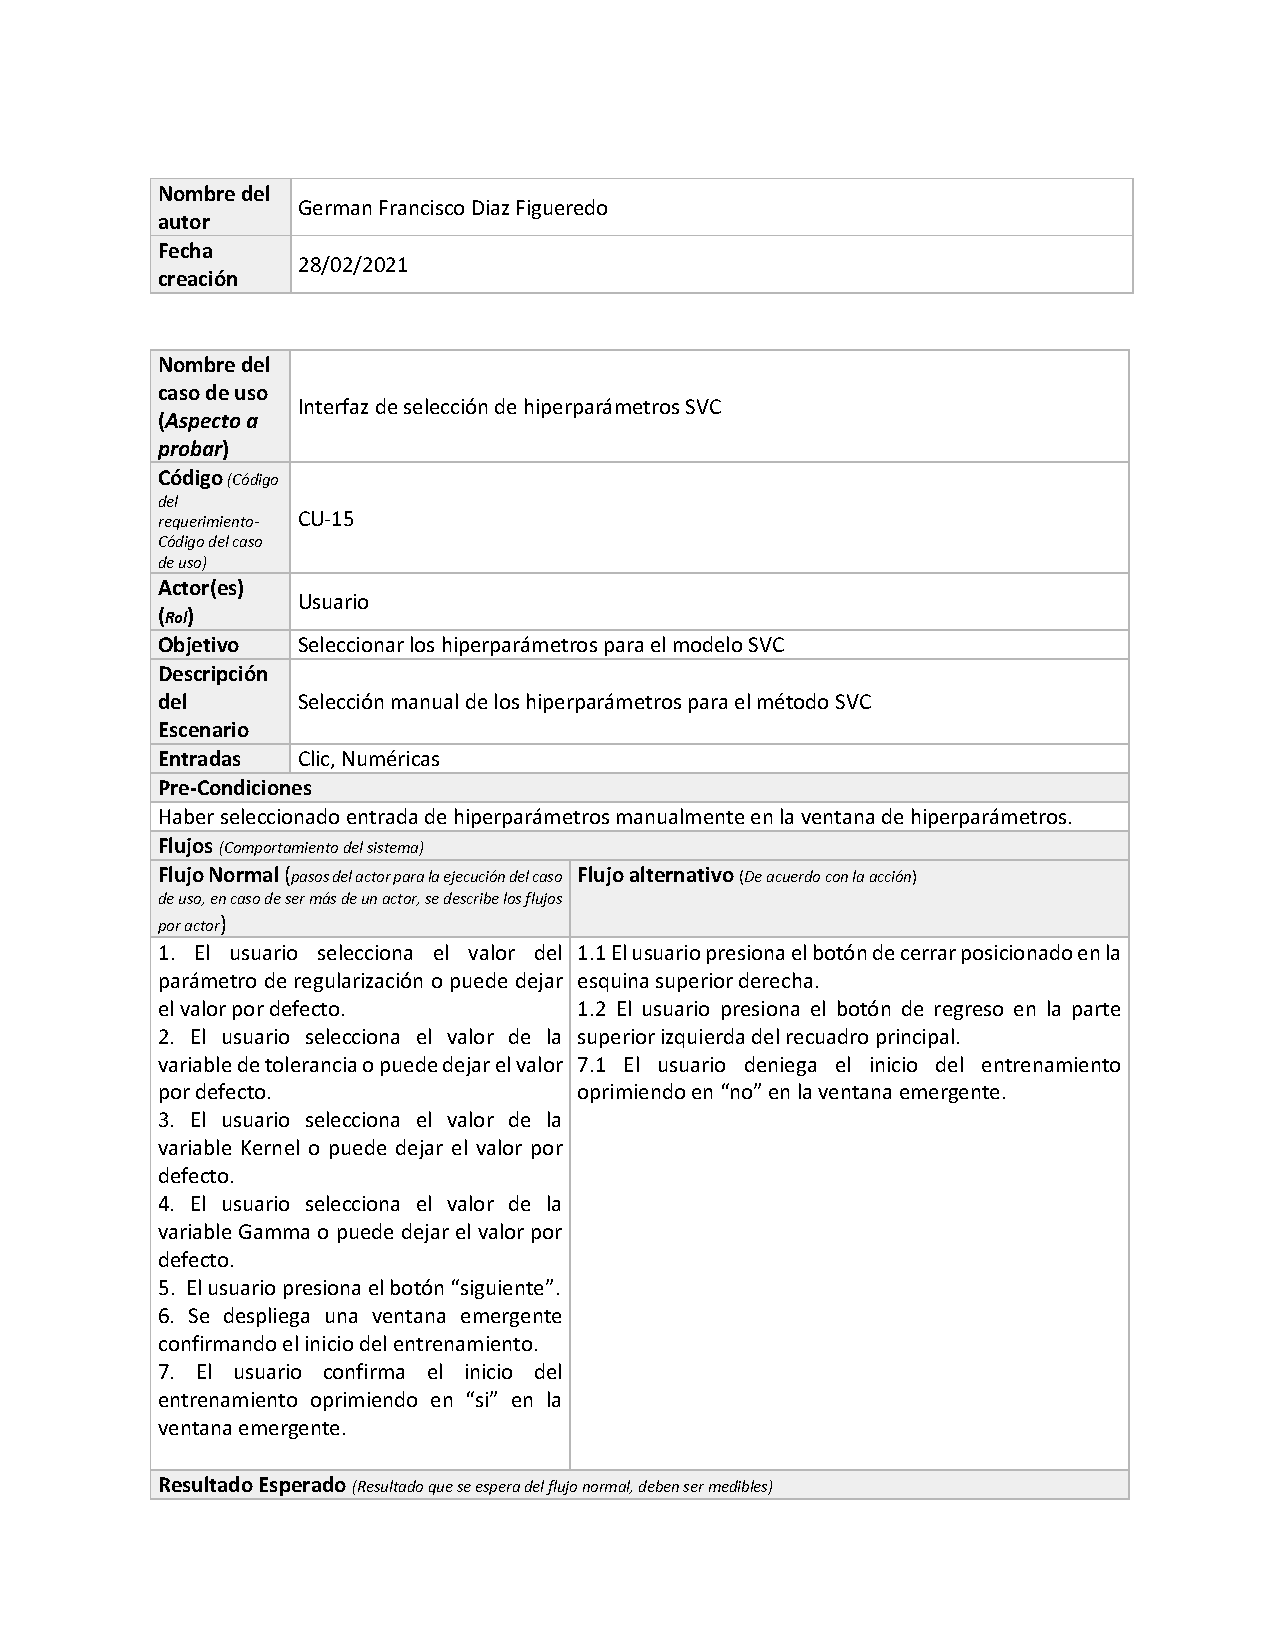
\includepdf[pages=-, pagecommand=\thispagestyle{otherplain}, width=\textwidth]{pdfs/CU-15_Firmado.pdf}
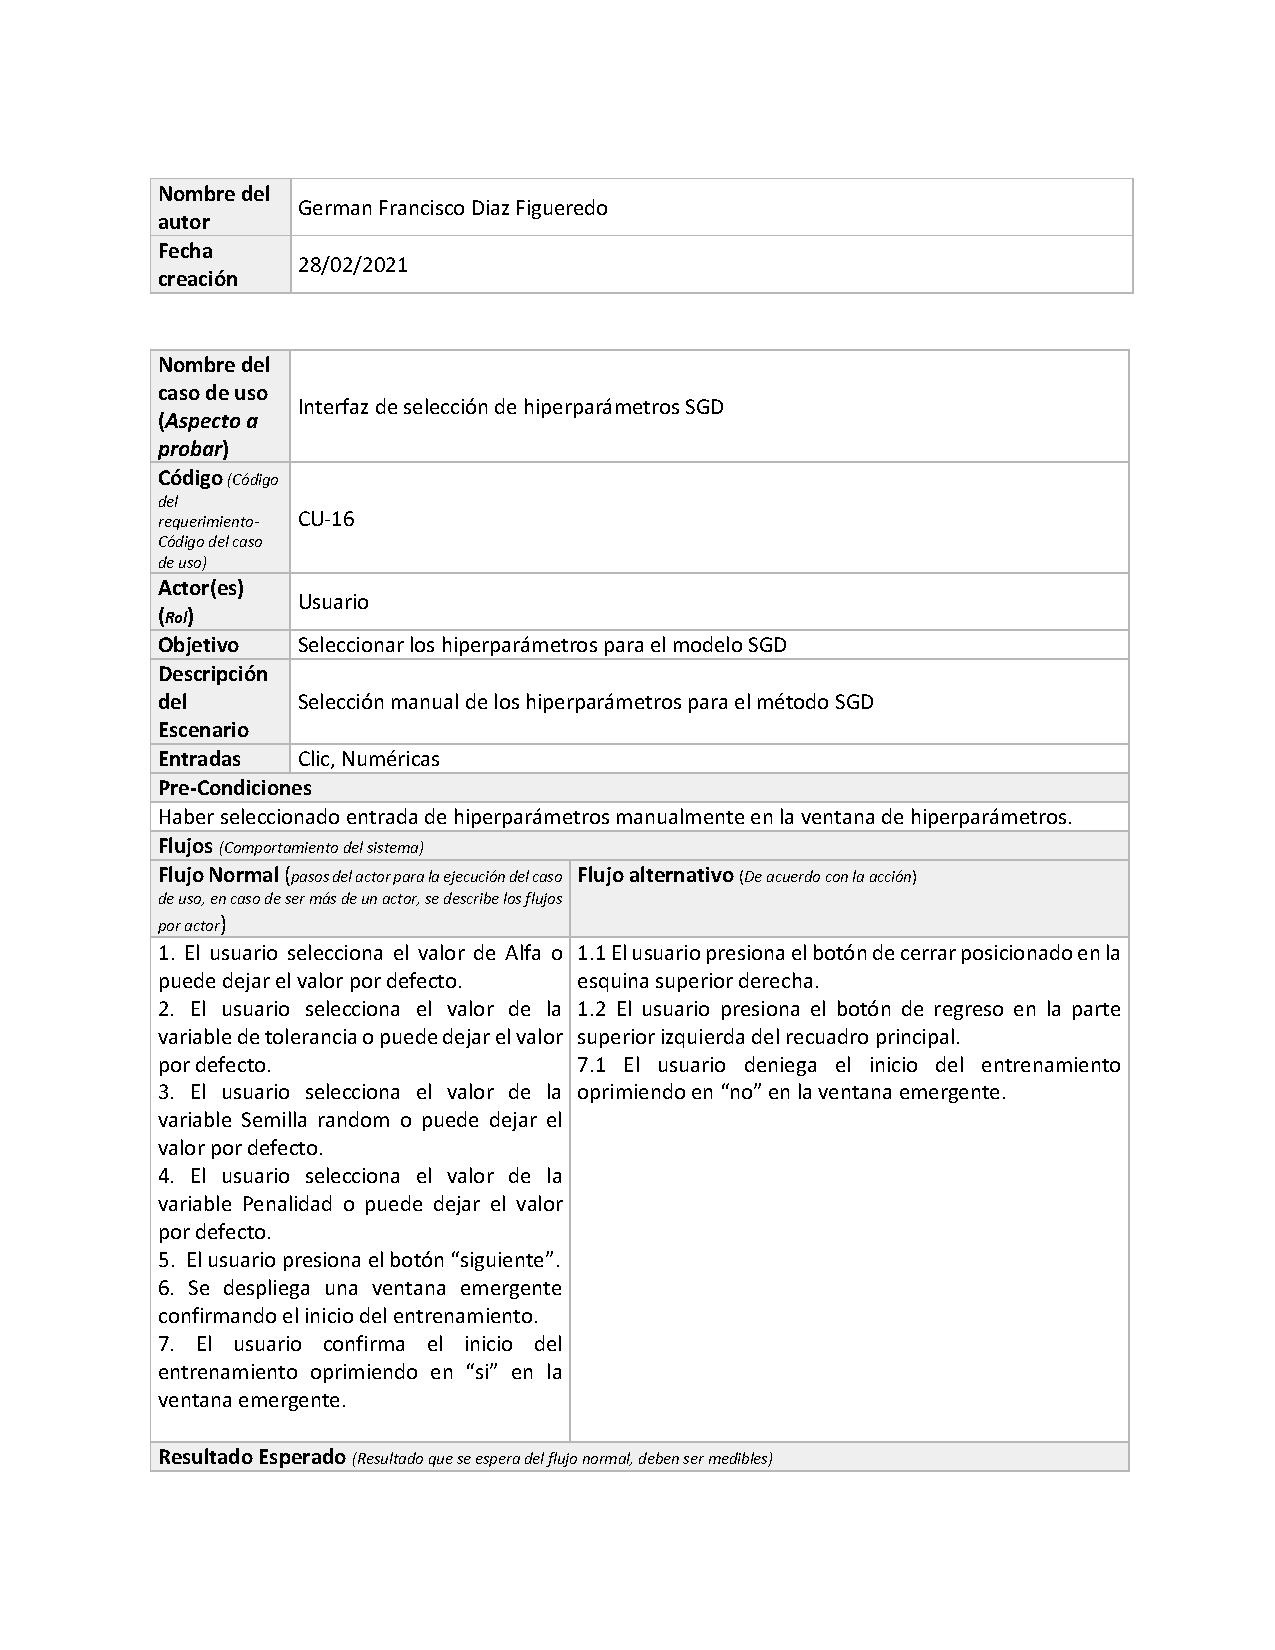
\includepdf[pages=-, pagecommand=\thispagestyle{otherplain}, width=\textwidth]{pdfs/CU-16_Firmado.pdf}
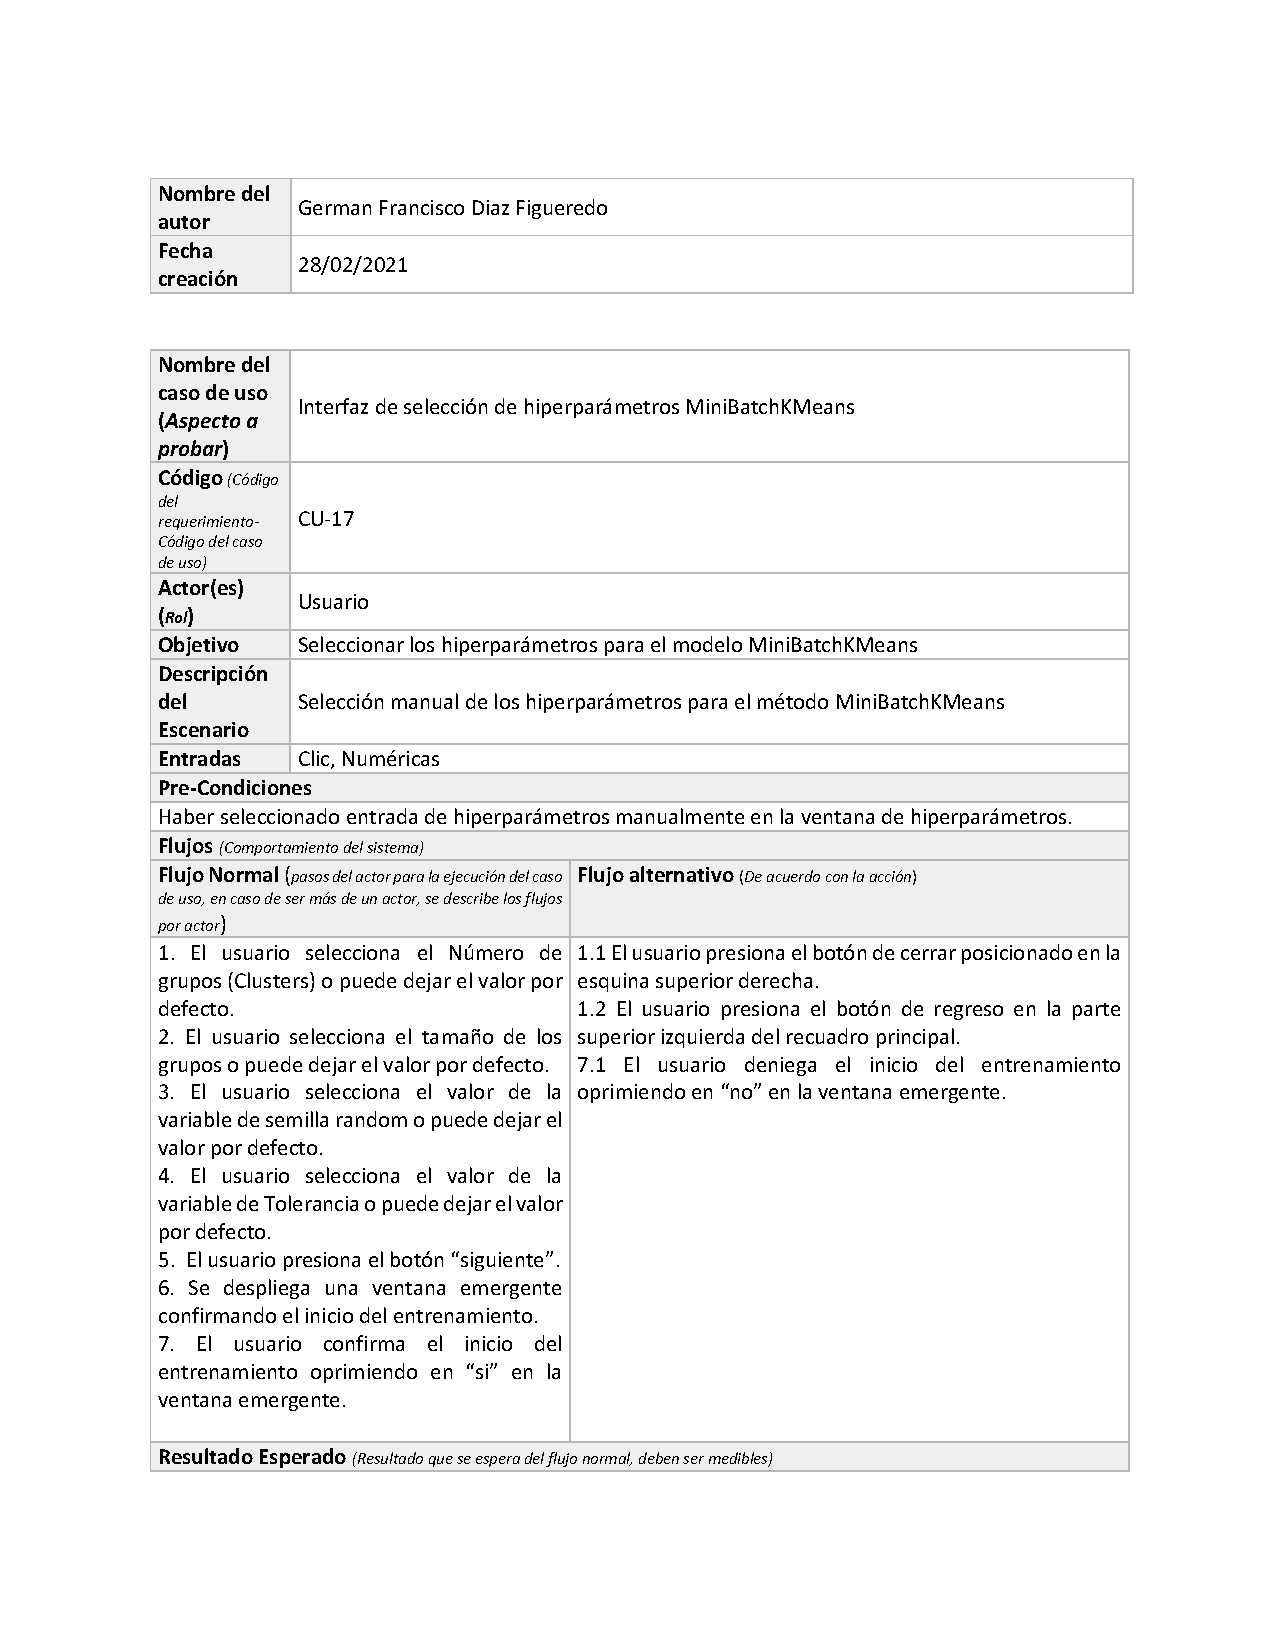
\includepdf[pages=-, pagecommand=\thispagestyle{otherplain}, width=\textwidth]{pdfs/CU-17_Firmado.pdf}
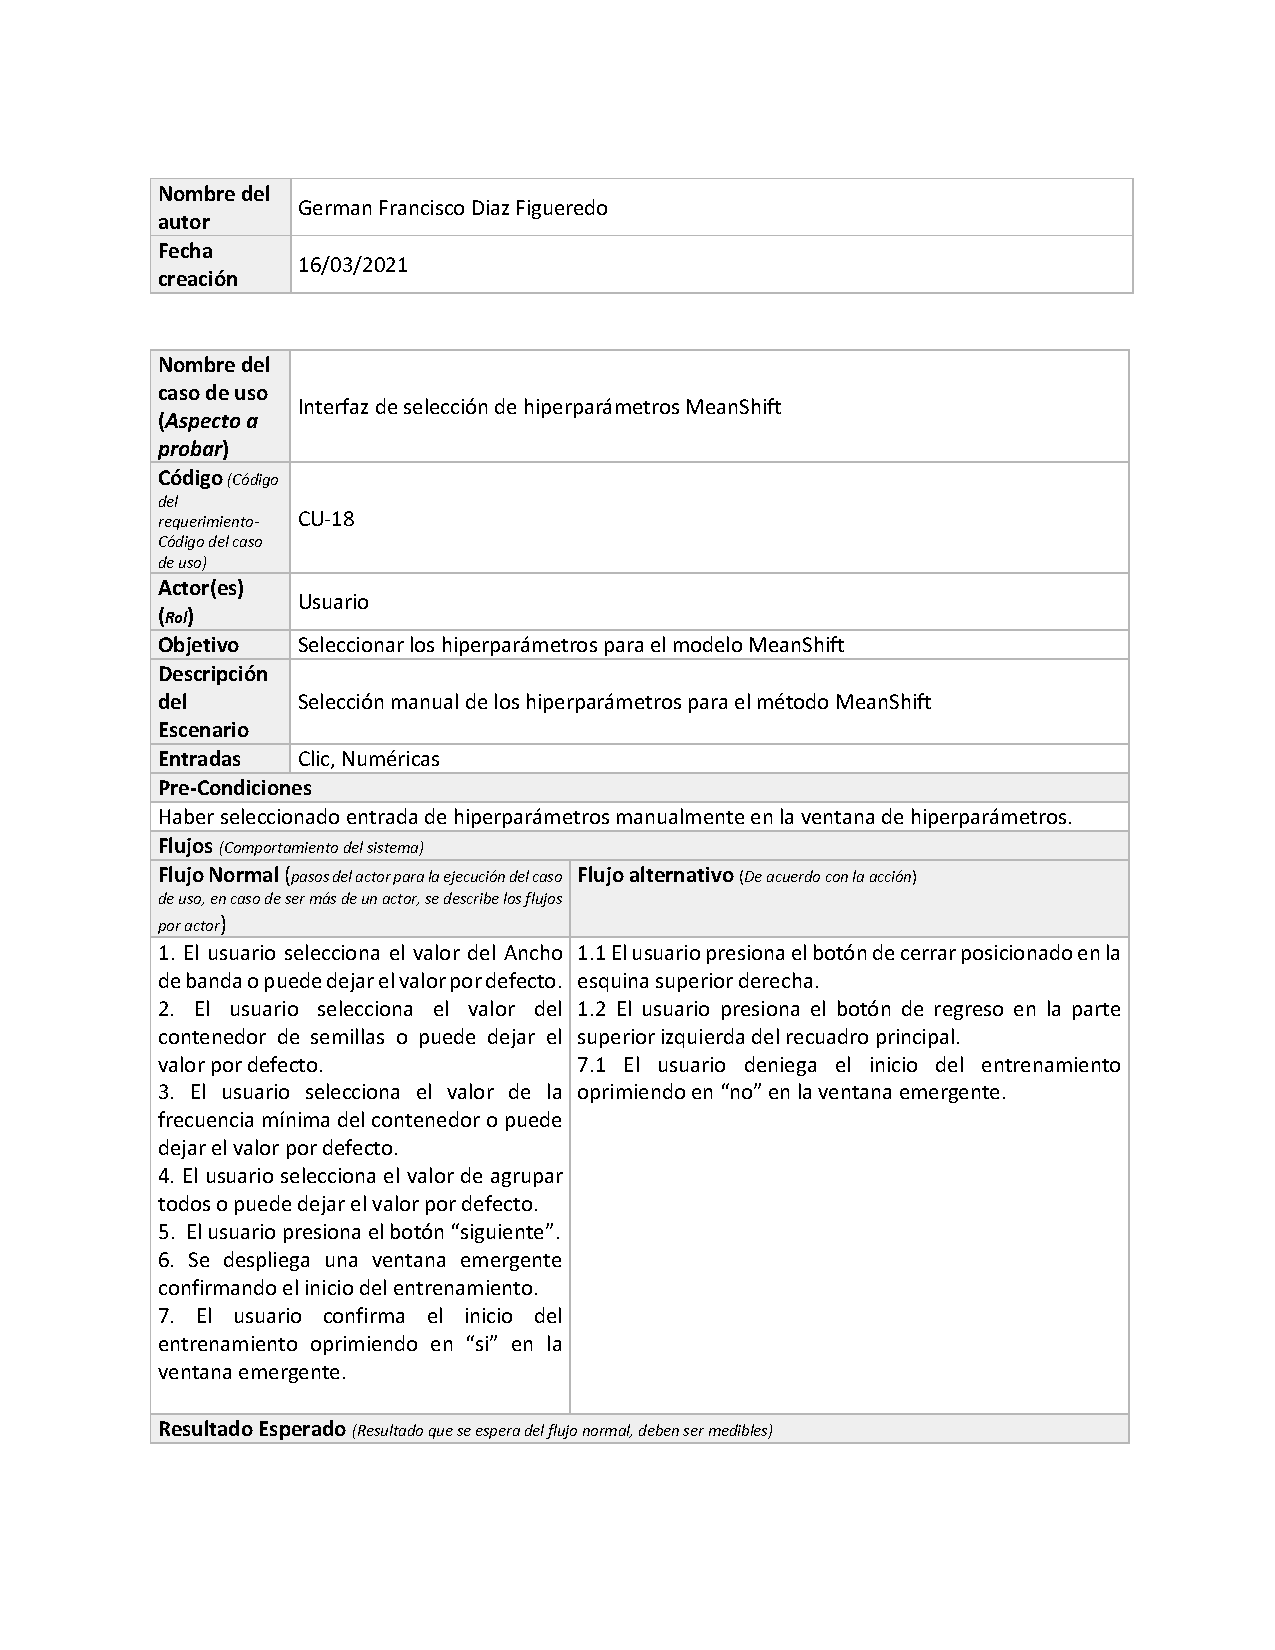
\includepdf[pages=-, pagecommand=\thispagestyle{otherplain}, width=\textwidth]{pdfs/CU-18_Firmado.pdf}
\includepdf[pages=-, pagecommand=\thispagestyle{otherplain}, width=\textwidth]{pdfs/CU-19_Firmado.pdf}
\includepdf[pages=-, pagecommand=\thispagestyle{otherplain}, width=\textwidth]{pdfs/CU-20_Firmado.pdf}
\includepdf[pages=-, pagecommand=\thispagestyle{otherplain}, width=\textwidth]{pdfs/CU-21_Firmado.pdf}
\includepdf[pages=-, pagecommand=\thispagestyle{otherplain}, width=\textwidth]{pdfs/CU-22_Firmado.pdf}
\includepdf[pages=-, pagecommand=\thispagestyle{otherplain}, width=\textwidth]{pdfs/CU-23_Firmado.pdf}
\includepdf[pages=-, pagecommand=\thispagestyle{otherplain}, width=\textwidth]{pdfs/CU-24_Firmado.pdf}
\includepdf[pages=-, pagecommand=\thispagestyle{otherplain}, width=\textwidth]{pdfs/CU-25_Firmado.pdf}

\end{document}